\begin{thwbr}
\chapter{โปรแกรมคำสั่งพื้นฐาน}
\begin{flushright}
{\it\latintext ``Write programs that do one thing and do it well.\\
Write programs to work together. \\
Write programs to handle text streams, \\
because that is a universal interface.''}\\
{{\bf\latintext  Doug McIlroy}}
\end{flushright}

ในลินุกซ์จะเป็นเพียงแค่ระบบปฏิบัติที่ไร้ค่าถ้าไม่โปรแกรมต่างๆใช้ร่วมกัน. โปรแกรมต่างๆที่ว่านี้ได้แก่โปรแกรมเสรีแบบบรรทัดคำสั่ง (command line) และโปรแกรมแบบ GUI. 

ตั้งแต่เริ่มต้นของระบบปฏิบัติการยูนิกซ์ซึ่งเป็นเวลานานกว่า 30 ปีแล้วโปรแกรมคำสั่งต่างๆที่ใช้ในตอนนั้นก็ยังใช้กันอยู่ในตอนนี้. โปรแกรมคำสั่งชื่อเดียวกันในสมัยในอาจจะมีส่วนที่เหมือนกันและแตกต่างกันกับโปรแกรมคำสั่งสมัยนี้ที่มีความสามารถเพิ่มเติมต่างๆมากขึ้น, ทำงานได้ดีขึ้น. แต่สิ่งที่ยังคงไว้อยู่คือโปรแกรมส่วนใหญ่ใช้ประมวลผลข้อมูลเท็กซ์, แสดงผลให้ผู้ใช้เป็นเท็กซ์ และใช้อินเทอร์เฟสแบบบรรทัดคำสั่ง. แน่นอนว่าการแสดงผลและรับข้อมูลเป็นเท็กซ์มีขีดจำกัด, และบางกรณีไม่สะดวกต่อการใช้จึงมีการสร้างอินเทอร์เฟสแบบหน้าต่างที่เรียกว่า X วินโดว์เสริมขึ้นจนเป็นอินเทอร์เฟสกึ่งมาตรฐานที่ใช้กันในลินุกซ์. 

ในบทนี้จะแนะนำโปรแกรมต่างๆที่มีในระบบลินุกซ์ซึ่งส่วนมากจะเป็นโปรแกรมบรรทัดคำสั่ง, และโปรแกรม GUI เป็นกรณีไป.

\medskip
%\section{แพ็กเกจ coreutils}
จากที่ได้แนะนำไปแล้วในบทที่ 1 ว่า Free Software Foundation หรือ GNU เป็นองค์กรณ์ที่มีบทบาทสำคัญอย่างยิ่งต่อลินุกซ์เพราะเป็นองค์กรณ์ที่สร้างหรือเป็นผู้สนับสนุนโครงการโปรแกรมพื้นฐานหลักที่ใช้กันในระบบปฏิบัติการยูนิกซ์ให้มีใช้ในลินุกซ์อย่างเสรี. แพ็กเกจที่สำคัญและเป็นพื้นฐานที่ลินุกซ์ทุกค่ายใช้ได้แก่ coreutils ซึ่งในแพ็กเกจนี้ยังแบ่งย่อยออกเป็น fileutils, shellutils และ textutils. 

\section{แพ็กเกจ fileutils}
แพ็กเกจ fileutils เป็นแพ็กเกจที่รวมโปรแกรมบรรทัดคำสั่งที่เกี่ยวกับการจัดการไฟล์ซึ่งในบทที่ผ่านมาได้แนะนำคำสั่งที่ใช้บ่อยและคำสั่งที่จำเป็นไปแล้วพอสมควร. ในตารางที่ \ref{tab:fileutils}

\begin{longtable}{lp{.55\textwidth}l}
\caption{โปรแกรมคำสั่งในแพ็กเกจ fileutils.}\label{tab:fileutils}\\
\toprule
\multicolumn{1}{c}{คำสั่ง} & \multicolumn{1}{c}{คำอธิบาย} & \multicolumn{1}{c}{อ้างอิง}\\
\midrule
\cmd{chgrp} & เปลี่ยนกลุ่มของไฟล์. & หน้า \pageref{cmd:chgrp}\\
\cmd{chown} & เปลี่ยนเจ้าของไฟล์. & หน้า \pageref{cmd:chown}\\
\cmd{chmod} & เปลี่ยนสิทธิ์การใช้ไฟล์. & หน้า \pageref{cmd:chmod}\\
\cmd{cp} & ก็อปปี้ไฟล์. & หน้า \pageref{cmd:cp}\\
\cmd{dd} & ก็อปปี้และแปลงข้อมูล. & หน้า \pageref{cmd:dd}\\
\cmd{df} & แสดงพื้นที่การใช้งานฮาร์ดดิสก์. & หน้า \pageref{cmd:df}\\
\cmd{dir} & แสดงรายการไฟล์. & \\
\cmd{dircolors} & ตั้งค่าเริ่มต้นเพื่อให้คำสั่ง \cmd{ls} แสดงสีต่างๆได้. &\\
\cmd{du} & แสดงพื้นที่การใช้งานฮาร์ดดิสก์. & หน้า \pageref{cmd:du}\\
\cmd{install} & ก็อปปี้ไฟล์และตั้งค่าสิทธิ์การใช้ไฟล์.& หน้า \pageref{cmd:install}\\
\cmd{ln} & สร้างลิงค์. & หน้า \pageref{cmd:ln}\\
\cmd{ls} & แสดงรายการไฟล์. & หน้า \pageref{cmd:ls}\\
\cmd{mkdir} & สร้างไดเรกทอรี. & หน้า \pageref{cmd:mkdir}\\
\cmd{mkfifo} & สร้างไฟล์ fifo. & หน้า \pageref{cmd:mkfifo}\\
\cmd{mknod} & สร้างไฟล์พิเศษ. &\\
\cmd{mv} & ย้ายไฟล์. & หน้า \pageref{cmd:mv}\\
\cmd{rm} & ลบไฟล์. & หน้า \pageref{cmd:rm}\\
\cmd{rmdir} & ลบไดเรกทอรีว่าง.& หน้า \pageref{cmd:rmdir}\\
\cmd{shred} & ทำลายข้อมูลในไฟล์.& หน้า \pageref{cmd:shred}\\
\cmd{sync} & เขียนข้อมูลที่อยู่ใน buffer ลงดิสก์.& หน้า \pageref{cmd:sync}\\
\cmd{touch} & เปลี่ยน timestamp ของไฟล์.& หน้า \pageref{cmd:touch}\\
\cmd{vdir} & แสดงรายการไฟล์.& \\
\bottomrule
\end{longtable}

\subsection{สำรวจพื้นที่ฮาร์ดดิสก์}
ถ้าอ่านจากคำอธิบายจากตารางที่ \ref{tab:fileutils} จะเห็นว่า \cmd{du} และ \cmd{df} ทำงานคล้ายๆกัน. คำสั่ง \cmd{df} จะแสดงพื้นที่ฮาร์ดดิสก์แบ่งตามดีไวซ์ต่างๆ, ส่วนคำสั่ง \cmd{du} จะแสดงพื้นที่ใช้งานของไดเรกทอรี่ที่ต้องการ.

\begin{MyExample}[สำรวจพื้นที่ฮาร์ดดิสก์ด้วย \cmd{df} และ \cmd{du}.]
\begin{MyEx}
$ \cin{df -h}
Filesystem            Size  Used Avail Use% Mounted on
/dev/hdb1              19G   13G  4.6G  74% /
/dev/hdb2              18G   13G  4.7G  73% /home
none                  442M     0  442M   0% /dev/shm
/dev/cdrom            3.2G  3.2G     0 100% /mnt/cdrom
$ \cin{du -sh $HOME}
13G     /home/poonlap
\end{MyEx}
\end{MyExample}%$

\subsection{ก็อปปี้ไฟล์}
คำสั่งสำหรับก็อปปี้ไฟล์ที่ใช้ทั่วไปคือ \cmd{cp}. ส่วนคำสั่ง \cmd{install} ก็ทำงานเหมือนกับคำสั่ง \cmd{cp} และวิธีใช้งานเบื้องต้นก็เหมือนกันคือก็อปปี้ไฟล์จากที่หนึ่งไปอีกที่หนึ่ง. คำสั่ง \cmd{install} มักใช้ในการติดตั้งโปรแกรมในระบบ. 

การติดตั้งโปรแกรมแบบง่ายที่สุดในระบบยูนิกซ์และลินุกซ์คือการก็อปปี้ไฟล์ไปไว้ในไดเรกทอรีเดียวกันกับไดเรกทอรีที่กำหนดในตัวแปรสภาพแวดล้อม \cmd{PATH} เช่น \cmd{/usr/bin}. ดิสทริบิวชันแต่ละค่ายอาจจะมีโปรแกรมสำหรับติดตั้งโปรแกรมที่มาเป็นแพ็กเกจต่างๆกันเช่น \cmd{rpm}, \cmd{dpkg}, \cmd{emerge} ฯลฯ. โปรแกรมติดตั้งแพ็กเกจเหล่านี้ก็ใช้การก็อปปี้ไฟล์โปรแกรมและไฟล์ที่เกี่ยวข้องอื่นๆไปไว้ที่ต้องการเท่านั้นเอง, และมีการสร้างฐานข้อมูลสำหรับควบคุมและติดตามการติดตั้งแพ็กเกจต่างๆ. การก็อปปี้ไฟล์จะใช้คำสั่ง \cmd{cp} ก็ได้แต่ถ้ามีการตั้งค่าต่างๆเช่นสิทธิ์การใช้ไฟล์, เจ้าของไฟล์ด้วยก็ต้องมาสั่งคำสั่ง \cmd{chmod}, \cmd{chown} ภายหลัง. ดังนั้นจึงมีคำสั่ง \cmd{install} เพื่อตั้งค่าต่างๆเหล่านี้พร้อมกับการก็อปปี้.

สำหรับโปรแกรมที่เป็นไฟล์ไบนารี, ไฟล์นั้นอาจจะมีข้อมูลที่ไม่จำเป็นในการใช้งานเช่นข้อมูลที่เกี่ยวกับการ debug%
\myvocab{d}{debug}{การกำจัดข้อมผิดพลาดของโปรแกรม. ข้อผิดพลาดนี้มักเป็นข้อผิดพลาดที่ไม่คาดคิดจนกระทั่งใช้งานจริงที่เรียกว่า runtime error.}%
 ในไฟล์. ข้อมูลเหล่านี้สร้างขึ้นตอนที่คอมไพล์โปรแกรมนั้นๆ. คำสั่ง \cmd{install}\cindex{install}\refcmd{install} ยังช่วยเอาข้อมูลที่ไม่จำเป็นเหล่านี้ออกด้วยเวลาติดตั้งด้วยตัวเลือก \cmd{-s}.\mymemo{การเอาของมูลที่ไม่จำเป็นสำหรับการรันโปรแกรมนี้เรียกว่า strip.} ถ้าไม่ใช้ตัวเลือกนี้, ก็อาจจะใช้คำสั่ง \cmd{strip}\cindex{strip} เอาข้อมูลที่ไม่จำเป็นออกไปต่างหาก. 

สมมติว่าเรามีไฟล์โปรแกรมไบนารีที่คอมไพล์เองและต้องการก็อปปี้เป็นชื่อ \cmd{myprogram} ไว้ที่ \cmd{\$HOME/bin} เพื่อใช้งาน. เราสามารถใช้คำสั่ง \cmd{install} แทนคำสั่ง \cmd{cp} ได้ตามตัวอย่างต่อไปนี้.
\begin{MyExample}[การใช้คำสั่ง \cmd{install}.]\label{ex:install}
\begin{MyEx}
$ \cin{ls -lF a.out}
-rwxr-xr-x    1 poonlap  users       14596 Sep  3 00:37 a.out*
$ \cin{install -vs -m 750 a.out ~/bin/myprogram}
`a.out' -> `/home/poonlap/bin/myprogram'
$ \cin{ls -lF a.out ~/bin/myprogram}
-rwxr-x---    1 poonlap  users        3116 Sep  3 00:41 /home/poonlap/bin/myprogram*
-rwxr-xr-x    1 poonlap  users       14596 Sep  3 00:38 a.out*
\end{MyEx}
\end{MyExample}%$
ตัวเลือก \cmd{-v} เป็นตัวเลือกที่ใช้ได้กับคำสั่ง \cmd{cp} คือแสดงสถานะการทำงาน. ตัวเลือก \cmd{-m} เป็นการระบุโหมดของไฟล์ที่ต้องการติดตั้ง. ให้สังเกตขนาดของไฟล์และโหมดของไฟล์ก่อนและหลังการก็อปปี้.


\subsection{เปลี่ยนเจ้าของไฟล์และกลุ่ม}
การเปลี่ยนเจ้าของไฟล์จะใช้คำสั่ง \cmd{chown}. ส่วนการเปลี่ยนกลุ่มของไฟล์จะใช้คำสั่ง \cmd{chgrp}. ถ้าต้องการเปลี่ยนทั้งเจ้าของไฟล์และกลุ่มไฟล์, สามารถใช้คำสั่ง \cmd{chown} เปลี่ยนค่าที่ต้องการในรวดเดียวโดยระบุเจ้าของไฟล์และชื่อกลุ่มโดยใช้เครื่องหมาย colon คั่นเช่นถ้าต้องการให้ไดเรกทอรี \cmd{/var/www} เป็นที่เก็บไฟล์สำหรับเว็บเซิฟร์เวอร์ให้มีเจ้าของเป็น apache และอยู่ในกลุ่ม users ให้ทำดังนี้.
\begin{MyExample}[การเปลี่ยนเจ้าของไฟล์และกลุ่มในคราวเดียวกัน.]
\begin{MyEx}
# \cin{chown -R apache:users /var/www}
\end{MyEx}
\end{MyExample}

\subsection{สร้างไฟล์พิเศษ}
เราได้รู้จักกับคำสั่งที่สร้างไฟล์พิเศษจากบทที่ผ่านมาเช่นถ้าต้องการสร้างไฟล์ fifo จะใช้คำสั่ง \cmd{mkfifo}. ถ้าต้องการสร้างลิงค์จะใช้คำสั่ง \cmd{ln}. คำสั่ง \cmd{mknod}\cindex{mknod}\refcmd{mknod} เป็นอีกคำสั่งหนึ่งที่ใช้สร้างไฟล์พิเศษได้แก่ ไฟล์ fifo, ไฟล์ดีไวซ์แบบ character และแบบ block. ผู้ใช้ทั่วไปสามารถสร้างไฟล์ fifo ได้ด้วยคำสั่ง \cmd{mkfifo} หรือ \cmd{mknod} ก็ได้. ส่วนการสร้างไฟล์ดีไวซ์ทำได้โดย root เท่านั้น. 

\subsection{ทำลายข้อมูล}
ในระบบปฏิบัติการตระกูลยูนิกซ์, การลบไฟล์ด้วยคำสั่ง \cmd{rm} นั้นเป็นเพียงแค่การลบฮาร์ดลิงค์ออกจากไดเรกทอรีเท่านั้น. เนื้อหาในไฟล์นั้นยังคงในที่ใดที่หนึ่งในฮาร์ดดิสก์จนกว่าพื้นที่นั้นจะถูกใช้เก็บข้อมูลใหม่. และในตอนนั้นข้อมูลตรงนั้นก็จะถูกแทนที่ด้วยข้อมูลใหม่. คำสั่ง \cmd{shred}\cindex{shred}\refcmd{shred}\mymemo{\cmd{shred} มาจากคำว่า shredder คือเครื่องทำลายเอกสาร.} เป็นคำสั่งทำลายข้อมูลในไฟล์โดยที่เขียนข้อมูลปลอมๆซ้ำกันหลายครั้งลงในไฟล์ที่ต้องการ. ถ้าใช้ตัวเลือก \cmd{-u} ประกอบด้วยจะทำการลบไฟล์นั้นหลังจากที่ทำลายข้อมูลเรียบร้อยแล้ว.

\subsection{\cmd{sync}}
การอ่านหรือเขียนข้อมูลลงดิกส์จะช้ากว่าการอ่านหรือเขียนข้อมูลลงหน่วยความจำ. ดังนั้นระบบปฏิบัติการสมัยใหม่จะใช้หน่วยความจำบางส่วนเก็บข้อมูลชั่วคราวเวลาเขียนข้อมูลลงไฟล์หรืออ่านข้อมูลลงไฟล์. เราเรียกหน่วยความจำที่ใช้ในลักษณะนี้ว่า \emph{buffer cache}\gindex{buffer cache}. การทำงานของ buffer cache จะเห็นชัดมากในกรณีที่ใช้ฟล็อปปี้. บางครั้งเราเขียนข้อมูลลงในฟล็อปปี้, ระบบจะไม่บันทึกข้อมูลที่เขียนลงในแผ่นฟล็อปปี้ทันทีแต่จะเก็บไว้ใน buffer cache. เวลาสั่งคำสั่ง \cmd{umount} แล้วจึงจะย้ายข้อมูลที่อยู่ในหน่วยความจำที่ต้องบันทึกลงในแผ่นฟล็อปปี้. การใช้คำสั่ง \cmd{sync} เป็นการบังคับเขียนข้อมูลที่อยู่ในหน่วยความจำลงในดิสก์. โดยปรกติผู้ใช้ไม่จำเป็นต้องใช้คำสั่งนี้เพราะลินุกซ์จะจัดการให้โดยอัตโนมัติอยู่แล้ว.





\section{แพ็กเกจ shellutils}
จากบทที่ผ่านมาเราทราบแล้วว่าคำสั่งที่ใช้ในเชลล์แบ่งเป็นคำสั่งประกอบภายใน (builtin command) และโปรแกรมคำสั่งที่มีอยู่ในระบบ. แพ็กเกจ shellutils เป็นแพ็กเกจที่รวมโปรแกรมคำสั่งที่ช่วยเสริมการทำงานของเชลล์ให้ใช้งานสะดวกยิ่งขึ้น, และคำสั่งหลายตัวมักใช้ประกอบในการเขียนเชลล์สคริปต์. 

โปรแกรมคำสั่งหลายตัวในแพ็กเกจนี้ถูกรวมอยู่ในคำสั่งประกอบภายในเชลล์ bash ด้วยเช่น \cmd{test}, \cmd{echo} ฯลฯ. หมายความว่าถ้าเราสั่งคำสั่ง \cmd{echo}, เชลล์จะเป็นตัวดำเนินงานเอง, ไม่ได้ใช้ไฟล์โปรแกรม \cmd{/bin/echo}. เดิมทีคำสั่งเหล่านี้ไม่ได้เป็นคำสั่งประกอบภายในเชลล์แต่มีการปรับปรุงเชลล์ bash ให้เอาคำสั่งเหล่านี้เป็นคำสั่งประกอบภายในด้วย. ในแพ็กเกจ shellutils ยังคงต้องเก็บโปรแกรมคำสั่งเหล่านี้ไว้เพื่อให้เข้ากันได้กับเชลล์อื่นและเชลล์ bash รุ่นเก่าๆ. 

\begin{longtable}{lp{.55\textwidth}l}
\caption{โปรแกรมคำสั่งในแพ็กเกจ shellutils.}\label{tab:shellutils}\\
\toprule
\multicolumn{1}{c}{คำสั่ง} & \multicolumn{1}{c}{คำอธิบาย} & \multicolumn{1}{c}{อ้างอิง}\\
\midrule
\cmd{[} & ตรวจสอบชนิดของไฟล์และเปรียบเทียบค่า. & หน้า \pageref{cmd:test}\\
\cmd{basename} & ลบส่วนที่อยู่หน้าชื่อไฟล์ออกและให้ผลลัพธ์เฉพาะชื่อไฟล์อย่างเดียว. & หน้า \pageref{cmd:basename}\\
\cmd{chroot} & เปลี่ยนไดเรกทอรีรูท.&\\
\cmd{date} & แสดงหรือตั้งเวลา, วันที่.& หน้า \pageref{cmd:date}\\
\cmd{dirname} & ตัดส่วนที่เป็นชื่อไฟล์ออกและแสดงเฉพาะส่วนที่อยู่หน้าชื่อไฟล์.& หน้า \pageref{cmd:dirname}\\
\cmd{echo} & แสดงบรรทัดข้อความ.& หน้า \pageref{cmd:echo}\\
\cmd{env} & แสดงหรือแก้ไขตัวแปรสภาพแวดล้อม.& หน้า \pageref{cmd:env}\\
\cmd{expr} & ตีความนิพจน์ (expression).& หน้า \pageref{cmd:expr}\\
\cmd{factor} & หาตัวประกอบของจำนวนเต็ม.& หน้า \pageref{cmd:factor}\\
\cmd{false} & คืนค่าสถานะการจบการทำงานไม่สมบูรณ์ (false).& หน้า \pageref{cmd:false}\\
\cmd{groups} & แสดงกลุ่มที่ผู้ใช้อยู่.& หน้า \pageref{cmd:groups}\\
\cmd{hostid} & แสดงค่าเฉพาะของโฮส, เครื่องคอมพิวเตอร์.&\\
\cmd{hostname} & แสดงชื่อโฮส.& หน้า \pageref{cmd:hostname}\\
\cmd{id} & แสดง uid และ gid.& หน้า \pageref{cmd:id}\\
\cmd{logname} & แสดงชื่อล็อกอิน.& \\
\cmd{nice} & แก้ไขลำดับความสำคัญของการทำงานโปรเซส (scheduling).& หน้า \pageref{nice}\\
\cmd{nohup} & อนุญาติให้โปรแกรมที่ระบุทำงานต่อถึงแม้ผู้ใช้จะล็อกเอาท์ไปแล้วก็ตาม.& หน้า \pageref{cmd:nohup}\\
\cmd{pathchk} & ตรวจสอบว่าชื่อไฟล์สามารถใช้ในระบบอื่นๆ (พอร์ต) ได้หรือไม่.&\\
\cmd{pinky} & โปรแกรม finger.&\\
\cmd{printenv} & แสดงตัวแปรสภาพแวดล้อมและค่าของตัวแปร.& หน้า \pageref{cmd:printenv}\\
\cmd{printf} & จัดรูปข้อมูลแล้วแสดงผลข้อมูลนั้น.&\\
\cmd{pwd} & แสดงไดเรกทอรีที่ทำงานอยู่.& หน้า \pageref{cmd:pwd}\\
\cmd{seq} & แสดงลำดับจำนวนที่ระบุ.& หน้า \pageref{cmd:seq}\\
\cmd{sleep} & หยุดการทำงานชั่วคราวตามระยะเวลาที่กำหนด.&\\
\cmd{stty} & แสดงและตั้งค่าของเทอร์มินอล.& หน้า \pageref{cmd:stty}\\
\cmd{su} & เปลี่ยนผู้ใช้เป็นผู้ใช้คนอื่น.& หน้า \pageref{cmd:su}\\
\cmd{tee} & ส่งข้อมูลออกไปบันทึกในไฟล์ที่ต้องการ.&\\
\cmd{test} & ทดสอบนิพจน์.& หน้า \pageref{cmd:test}\\
\cmd{true} &  คืนค่าสถานะการจบการทำงานสมบูรณ์ (true).& หน้า \pageref{cmd:true}\\
\cmd{tty} & แสดงชื่อเทอร์มินอล.& หน้า \pageref{cmd:tty}\\
\cmd{uname} & แสดงข้อมูลของระบบปฏิบัติการ.& หน้า \pageref{cmd:uname}\\
\cmd{users} & แสดงชื่อผู้ใช้ที่ล็อกอินอยู่ในระบบ.& หน้า \pageref{cmd:users}\\
\cmd{who} & แสดงชื่อผู้ใช้ที่ล็อกอินอยู่ในระบบ.& หน้า \pageref{cmd:who}\\
\cmd{whoami} & แสดง id ที่ให้ผลจริง.& หน้า \pageref{cmd:whoami}\\
\cmd{yes} & แสดงสายอักขระที่ต้องการไปเรื่อยๆ. &\\
\bottomrule
\end{longtable}



\subsection{ตรวจสอบไฟล์และค่าต่างๆ}
คำสั่งที่ใช้ตรวจสอบไฟล์และค่าต่างๆได้แก่คำสั่ง \cmd{test}\refcmd{test} และคำสั่ง \cmd{[}. คำสั่งทั้งสองตัวเหมือนกันเพียงแต่มีไวยกรณ์ต่างกันตรงที่คำสั่ง \cmd{[} ต้องการเครื่องหมาย \cmd{]} ปิดท้ายเสมอ. โดยปรกติคำสั่ง \cmd{test} มักจะใช้ร่วมกับไวยกรณ์ \cmd{if} ของเชลล์เพื่อตรวจสอบไฟล์หรือค่าต่างๆ.

ตัวอย่างต่อไปนี้เป็นตัวอย่างการตรวจสอบไฟล์ว่ามีจริงหรือไม่ด้วยตัวเลือก \cmd{-e}.
\begin{MyExample}[ตรวจสอบว่ามีไฟล์หรือไม่.]
\begin{MyEx}
$ \cin{test -e /etc/passwd}
$ \cin{[ -e /etc/passwd ]}
\end{MyEx}
\end{MyExample}
เราจะเรียก ``\cmd{-e /etc/passwd}'' ว่าเป็น\emph{นิพจน์ (expression)}\myvocab{e}{expression}{\emph{นิพจน์}. ประโยคที่แสดงความหมายอย่างใดอย่างหนึ่ง.} และคำสั่ง \cmd{test} จะตรวจสอบว่านิพจน์นั้นจริงหรือเท็จ. คำสั่ง \cmd{test} จะไม่แสดงผลออกทางหน้าจอไม่ว่าจะจริงหรือเท็จ, แต่จะใช้ตัวแปรสถานะจบการทำงาน ``\cmd{\$?}'' บอกว่าจริงหรือเท็จ. ถ้าการตรวจสอบเป็นจริงจะมีค่าเป็น 0, ถ้าเป็นเท็จจะมีค่าเป็นค่าอื่นๆที่ไม่ใช่ 0. 

ตัวอย่างต่อไปนี้เป็นการตรวจสอบใช้คำสั่ง \cmd{test} ร่วมกับ \cmd{if}.
\begin{MyExample}[การใช้คำสั่ง \cmd{test} ร่วมกับ \cmd{if}.]
\begin{MyEx}
$ \cin{if}
> \cin{[ -f /etc/shadow -a `whoami` == root ]}
> \cin{then}
> \cin{echo You are root and file /etc/shadow existed.}
> \cin{else}
> \cin{echo You are not root or file /etc/shadow does not exist.}
> \cin{fi}
You are not root or file /etc/shadow does not exist.
\end{MyEx}
\end{MyExample}%$

คำสั่ง \cmd{if} จะตรวจสอบตัวแปรสถานะจบการทำงานถ้าเป็นจริงก็จะกระทำส่วนที่ต่อจาก \cmd{then} ถ้าเป็นเท็จก็จะกระทำส่วนที่ต่อจาก \cmd{else}. จากตัวอย่างมีการเชื่อมนิพจน์ด้วย \cmd{-a} ซึ่งนิพจน์ทั้งสองที่ถูกเชื่อมต้องเป็นจริงแล้วนิพจน์โดยรวมจะเป็นจริง.

คำสั่ง \cmd{test} สามารถตรวจสอบประเภทไฟล์, สิทธิ์การใช้ไฟล์เบื้องต้น, เปรียบเทียบค่าสายอักขระ, และเปรียบเทียบจำนวนเต็ม. รายละเอียดเหล่านี้ดูได้จากสรุปการใช้คำสั่งหน้า \pageref{cmd:test}.



\subsection{สกัดส่วนของชื่อไฟล์}
เวลาใช้เชลล์จะมีบางกรณีที่เราต้องการสกัดส่วนของชื่อไฟล์มาเพื่อกระทำการอย่างใดอย่างหนึ่ง. คำสั่งที่ช่วยแยกชื่อไฟล์หรือไดเรกทอรีจริงๆออกจากส่วนเป็นพาท (path) ของชื่อไฟล์คือคำสั่ง \cmd{basename}\cindex{basename}\refcmd{basename} และ \cmd{dirname}\cindex{dirname}\refcmd{dirname}. คำสั่งสองคำสั่งนี้ไม่ได้ทำอะไรมากเพียงแต่สกัดส่วนที่ต้องการให้เท่านั้น. มีประโยชน์เมื่อใช้เขียนเชลล์สคริปต์.

\begin{MyExample}[การสกัดชื่อไฟล์หรือไดเรกทอรีจากชื่อไฟล์แบบ full path.]
\begin{MyEx}
$ \cin{basename /usr/local/bin/test.pl}
test.pl
$ \cin{basename /usr/local/bin/test.pl .pl} \mycomment{\cmd{.pl} คือส่วนที่ต้องการตัดออกจากชื่อไฟล์.}
test
$ \cin{dirname /usr/local/bin/test.pl}
/usr/local/bin
$ \cin{basename /home/}
home \mycomment{ผลลัพธ์จะตัดเครื่องหมาย \cmd{\bs} ให้ด้วย.}
$ \cin{dirname /home/}
/
\end{MyEx}
\end{MyExample}%$

จากตัวอย่างจะเห็นว่าคำสั่ง \cmd{basename} สามารถสกัดเอาส่วนขยายชื่อไฟล์ออกได้ด้วยถ้าระบุตามหลังชื่อไฟล์. คำสั่งที่เกี่ยวกับชื่อไฟล์อีกตัวคือ \cmd{pathchk}\cindex{pathchk} ใช้สำหรับตรวจดูว่าชื่อไฟล์นั้นมีรูปแบบถูกต้องหรือไม่เช่นจำนวนอักษรที่ใช้ในชื่อไฟล์เกินขีดจำกัดหรือไม่เป็นต้น. คำสั่ง \cmd{pathchk} เป็นคำสั่งที่ไม่ค่อยใช้.
 
\subsection{ถูกผิด}
คำสั่ง \cmd{true}\cindex{true}\refcmd{true} และ \cmd{false}\cindex{false}\refcmd{false} ไม่ได้ทำอะไรเป็นพิเศษเพียงแต่ตั่งค่าสถานะจบการทำงานเป็น 0 (\cmd{true}) หรือ 1 \cmd{false} ตามต้องการ. มักจะใช้ในการเขียนเชลล์สคริปต์ใช้ในการตั้งค่าตัวแปรสถานะจบการทำงาน. ถ้าการทำงานจบบริบูรณ์ถูกต้องก็สั่งคำสั่ง \cmd{true} เป็นคำสั่งสุดท้าย. ถ้ามีข้อผิดพลาดก็สั่งคำสั่ง \cmd{false}.

\subsection{คำสั่งเกี่ยวกับข้อมูลของระบบ}
ในระบบปฏิบัติการลินุกซ์จะมีคำสั่งที่แสดงข้อมูลเบื้องต้นเกี่ยวกับระบบและผู้ใช้ในระบบหลายตัว. คำสั่งที่บอกว่าผู้ใช้ตอนนี้คือใครได้แก่ \cmd{id}, \cmd{whoami} และ \cmd{logname}\cindex{logname}. คำสั่ง \cmd{whoami} จะเหมือนกับการสั่งคำสั่ง ``\cmd{id -un}''. คำสั่ง \cmd{id} จะให้ข้อมูลเกี่ยวกับกลุ่มด้วย, ส่วนคำสั่ง \cmd{logname} จะแสดงเฉพาะชื่อล็อกอินเท่านั้น. ถ้าต้องการดูแค่กลุ่มที่ตัวเองอยู่ก็ให้ใช้คำสั่ง \cmd{groups}\cindex{groups}\refcmd{groups}. 

คำสั่ง \cmd{hostid}\cindex{hostid} เป็นคำสั่งที่แสดงหมายเลขเฉพาะประจำเครื่อง. หมายเลขนี้จะไม่ซ้ำกับเครื่องอื่นๆและสามารถใช้ในการควบคุมการติดตั้งซอฟต์แวร์ที่ต้องการยึดติดกับเครื่อง. ซอฟต์แวร์บางตัวสามารถตรวจสอบ \cmd{hostid} เพื่อดูว่าเครื่องนั้นมีสิทธิ์รันซอฟต์แวร์นั้นได้หรือไม่. แต่ปัจจุบันไม่ค่อยใช้วิธีการตรวจสอบ \cmd{hostid} แล้วเพราะค่าเหล่าสามารถปลอมกันได้. คำสั่งที่เกี่ยวกับคอมพิวเตอร์อีกตัวคือ \cmd{hostname}\refcmd{hostname}\cindex{hostname} ใช้แสดงชื่อเครื่องหรือตั้งชื่อเครื่องคอมพิวเตอร์. ชื่อโฮสดังกล่าวจะใช้กับโปรแกรมที่เกี่ยวกับเน็ตเวิร์กต่างๆเพื่อระบุตัวเครื่อง. 

คำสั่งที่ใช้แสดงข้อมูลเบื้องต้นเกี่ยวกับเคอร์เนลได้แก่ \cmd{uname}\cindex{uname}\refcmd{uname}. โดยปรกติจะใช้กับตัวเลือก \cmd{-a} เพื่อแสดงข้อมูลทั้งหมดเช่น รุ่นของเคอร์เนล, สถาปัตยกรรมของเครื่อง, ข้อมูลเบื้องต้นของหน่วยประมวลผล ฯลฯ. ข้อมูลเหล่านี้มีความสำคัญเวลาใช้โปรแกรมหรือไดร์เวอร์ที่ขึ้นอยู่กับรุ่นของเคอร์เนล, เป็นวิธีที่ตรวจสอบว่าลินุกซ์ที่เราใช้อยู่นั้นใช้เคอร์เนลรุ่นไหนอยู่.

\subsection{สำรวจผู้ใช้ที่ล็อกอิน}
คำสั่งที่ใช้ตรวจสอบดูว่าขณะนี้มีใครบ้างที่ล็อกอินอยู่ในระบบได้แก่คำสั่ง \cmd{users} และ \cmd{who}. คำสั่ง \cmd{users} จะอาศัยข้อมูลจากไฟล์ \cmd{/var/run/utmp}\gindex{utmp@ไฟล์ \cmd{/var/run/utmp}} โดยปริยายหรืออาศัยข้อมูลจากไฟล์ \cmd{/var/log/wtmp}\gindex{wtmp@ไฟล์ \cmd{/var/log/wtmp}}. ไฟล์ \cmd{utmp} เป็นไฟล์ไบนารีที่เก็บข้อมูลผู้ใช้ที่กำลังอยู่ในระบบ. ส่วนไฟล์ \cmd{wtmp} เป็นไฟล์เก็บข้อมูลล็อกอินและล็อกเอาท์ของผู้ใช้, เวลาที่ระบบเริ่มทำงาน (startup) และจบการทำงาน (shutdown) ด้วย. คำสั่ง \cmd{users} จะแสดงแค่ชื่อล็อกอินของผู้ที่ล็อกอินอยู่ในระบบไม่มีข้อมูลอื่นเพิ่มเติม. เมื่อเทียบกับคำสั่ง \cmd{who}\cindex{who}\refcmd{who} จะให้ข้อมูลมากกว่าคำสั่ง \cmd{users}.


\begin{MyExample}[สำรวจผู้ใช้ที่ล็อกอินอยู่ในระบบด้วย \cmd{who}.]
\begin{MyEx}
$ \cin{who -Hu}
NAME     LINE         TIME         IDLE          PID COMMENT
poonlap  :0           Sep 13 19:53   ?          8395
poonlap  pts/2        Sep 13 19:54   .         10444 (:0.0)
poonlap  pts/3        Sep 13 21:05 00:24       10444 (:0.0)
poonlap  pts/4        Sep 13 21:05   .         10444 (:0.0)
root     pts/5        Sep 13 21:29   .         26565 (10.0.0.196)
\end{MyEx}
\end{MyExample}%$

เราสามารถรู้ได้ว่าผู้ใช้ล็อกอินเข้ามาทางไหนได้จากคอลัมน์ LINE และ COMMENT. คอลัมน์ LINE จะแสดงเทอร์มินอลที่ผู้ใช้ใช้อยู่. \cmd{pts}\gindex{pts} หมายถึง pseudo-terminal\gindex{pseudo-terminal}\mymemo{อ่าน \cmd{man pts} เกี่ยวกับรายละเอียดของ \cmd{pts}.} คือเทอร์มินอลเสมือนที่ใช้อยู่ในเทอร์มินอลเอมิวเลเตอร์. \cmd{:0} แสดงว่าผู้ใช้ล็อกอินผ่านทาง X Display Manager. ในคอลัมน์ COMMENT จะแสดง IP address ถ้าผู้ใช้ล็อกอินผ่านทางเน็ตเวิร์ก. ในคอลัมน์ TIME จะแสดงวันและเวลาที่ผู้ใช้ล็อกอิน. IDLE จะแสดงเวลาที่ว่างเฉย. เวลา IDLE นี้บอกให้เราทราบเวลาที่ผู้ใช้นั้นล็อกอินอยู่แต่ไม่ได้กระทำการใดๆในระบบ. PID จะแสดงหมายเลขโปรเซสของโปรแกรมที่ใช้หลังล็อกอิน.

คำสั่งที่คล้ายกับ \cmd{who} คือ \cmd{w}\cindex{w}\refcmd{w} แต่จะแสดงรายละเอียดเน้นการใช้งานของหน่วยประมวลผลและอ่านเข้าใจง่ายกว่าคำสั่ง \cmd{who}. 

\begin{MyExample}[ใช้คำสั่ง \cmd{w} ดูผู้ใช้ที่ล็อกอินและโปรแกรมที่ใช้.]
\begin{MyEx}
$ \cin{w}
 21:53:17 up  2:02,  5 users,  load average: 0.15, 0.28, 0.32
USER     TTY        LOGIN@   IDLE   JCPU   PCPU WHAT
poonlap  :0        19:53   ?xdm?  15:28   0.60s gnome-session
poonlap  pts/2     19:54    0.00s  2:11   0.00s w
poonlap  pts/3     21:05    2:35   0.00s  0.00s -bash
poonlap  pts/4     21:05   23:04  32.25s  0.67s xmms
root     pts/5     21:29   23:53   0.00s  0.00s -bash
\end{MyEx}
\end{MyExample}%$

ในบรรทัดแรกของคำสั่ง \cmd{w} จะแสดงเวลาปัจจุบัน, ระยะเวลาที่ระบบทำงานตั้งแต่เปิดเครื่อง, จำนวนผู้ใช้ที่ล็อกอินในระะบ, และ\emph{โหลดโดยเฉลี่ย (load average)}\myvocab{l}{load average}{\emph{โหลดโดยเฉลี่ย}. ค่าเฉลี่ยของจำนวนโปรเซสที่ active อยู่ในระบบ. ค่านี้จะแสดงให้ทราบว่าระบบยุ่งหรือไม่. ค่านี้ไม่จำเป็นต้องสัมพันธ์กับเปอร์เซ็นต์การใช้งานของหน่วยประมวลผล.}\gindex{load average} ในช่วงเวลา 1, 5 และ 15 นาทีที่ผ่านมา. บรรทัดถัดจากนั้นจะแสดงชื่อผู้ใช้ที่ล็อกอินและรายละเอียดต่างๆคล้ายกับคำสั่ง \cmd{who}. JCPU\gindex{jcpu@JCPU} คือระยะเวลาหน่วยประมวลใช้ไปกับโปรแกรมที่กระทำอยู่ในเทอร์มินอลนั้นไม่ว่าจะเป็นโปรเซส foreground หรือ background. PCPU\gindex{pcpu@PCPU} คือระยะเวลาหน่วยประมวลใช้ไปกับโปรแกรมที่กระทำอยู่ขณะนั้นในเทอร์มินอล, ได้แก่โปรแกรมที่แสดงในคอลัมน์ WHAT.

บรรทัดแรกของคำสั่ง \cmd{w} เป็นข้อมูลสถิติการทำงานระบบโดยทั่วไปซึ่งสามารถแสดงได้ด้วยคำสั่งต่างหากคือ \cmd{uptime}\cindex{uptime}\refcmd{uptime} ซึ่งจะให้ผลเหมือนกัน.

คำสั่งที่เกี่ยวข้องแต่ไม่ได้อยู่ในแพ็กเกจ shellutils อีกคำสั่งคือ \cmd{last}\cindex{last}\refcmd{last}.
\begin{MyExample}[ดูสถิติการล็อกอินด้วย \cmd{last}.]
\begin{MyEx}
$ \cin{last -n 5}
poonlap  pts/3        yahoobb219037040 Mon Sep 13 22:28   still logged in
xxxxx    pts/3        yahoobb219215060 Mon Sep 13 22:02 - 22:04  (00:01)
xxxxx    pts/1        yahoobb219215060 Mon Sep 13 21:59   still logged in
poonlap  pts/1        yahoobb219037040 Sun Sep 12 15:10 - 15:17  (00:07)
xxxxx    pts/1        yahoobb219215060 Sun Sep 12 12:15 - 12:21  (00:06)

wtmp begins Wed Sep  1 13:46:59 2004
\end{MyEx}
\end{MyExample}%$

คำสั่ง \cmd{last} จะแสดงเทอร์มินอลที่ใช้, IP address หรือชื่อโฮสที่ใช้ล็อกอินเข้ามา (ถ้ามี), และข้อมูลเวลาล็อกอินและล็อกเอาท์ของผู้ใช้แต่ละคน. เนื่องจากคำสั่ง \cmd{last} ใช้ข้อมูลจากไฟล์ \cmd{/var/log/wtmp} ดังนั้นจะมีข้อมูลเวลาเกี่ยวกับการรีบูต, เปิดเครื่อง, และปิดเครื่องด้วยถ้าใช้ร่วมกับตัวเลือก \cmd{-x}.

คำสั่งนี้ยังสามารถดูผู้ใช้ที่ใช้เทอร์มินอลที่ระบุได้ด้วย. ตัวอย่างเช่นเรามีเซิฟร์เวอร์อยู่ในห้องที่แยกต่างหากคนโดยทั่วไปไม่สามารถใช้คอนโซลได้ง่ายๆ. ถ้าต้องการดูชื่อผู้ใช้และเวลาของคนที่ใช้คอนโซลก็สามารถใช้คำสั่ง ``\cmd{last vc/1}''\mymemo{ชื่อเทอร์มินอลของคอนโซลในบางระบบอาจจะไม่ใช่ \cmd{vc/1} เช่นใน Debian จะเป็น \cmd{tty1}.} ระบุเทอร์มินอลเสมือน (คอนโซล) อันแรก (\cmd{Ctrl+Alt+F1}) ดูคนที่ใช้คอนโซลและเวลาได้.

ในกรณีที่ผู้ใช้ล็อกอินผิดพลาดเช่นพิมพ์ชื่อหรือรหัสผ่านผิด. ถ้าในระบบมีไฟล์ \cmd{/var/{\wbr}log/{\wbr}btmp}\mymemo{บางระบบไม่มีไฟล์ \cmd{btmp} อาจจะใช้ \cmd{touch} สร้างไฟล์นี้ให้ทำงานได้.}\gindex{btmp@ไฟล์ btmp}, ก็จะบันทึกความผิดพลาดที่เกี่ยวกับการล็อกอินไว้ด้วยในไฟล์นี้. ไฟล์ \cmd{btmp} เป็นไฟล์ประเภทเดียวกับ \cmd{utmp} และ \cmd{wtmp} คือเก็บข้อมูลเวลาเกี่ยวกับการล็อกอินล็อกเอาท์. ในระบบจะมีคำสั่ง \cmd{lastb}\mymemo{``b'' ย่อมาจาก bad.}\cindex{lastb} สำหรับดูว่าใครล็อกอินพลาดบ้าง.

\begin{MyExample}[ดูบันทึกล็อกอินที่ผิดพลาดด้วย \cmd{lastb}.]
\begin{MyEx}
$ \cin{lastb vc/1}
UNKNOWN  vc/1                          Mon Sep 13 22:50 - 22:50  (00:00)
nobody   vc/1                          Mon Sep 13 22:50 - 22:50  (00:00)
root     vc/1                          Mon Sep 13 22:50 - 22:50  (00:00)
poonlap  vc/1                          Mon Sep 13 22:49 - 22:49  (00:00)
 
btmp begins Mon Sep 13 22:49:35 2004
\end{MyEx}
\end{MyExample}%$

จากตัวอย่างคำสั่ง \cmd{lastb}, เราพอจะคาดเดาได้ว่ามีคนพยายามล็อกอินจากคอนโซลแต่ล็อกอินไม่ได้. ไม่ว่าจะเป็นรหัสผ่านไม่ถูกต้อง, หรือใช้ชื่อล็อกอินที่ระบบไม่รู้จัก (UNKNOWN).

\subsection{เทอร์มินอล}
เทอร์มินอลเป็นอินเทอร์เฟสที่ใช้ติดต่อกับเชลล์, รับข้อมูลนำเข้ามาตรฐาน stdin จากคีย์บอร์ดและส่งข้อมูลมาตรฐาน stdout ออกทางหน้าจอ. ในสมัยก่อนเทอร์มินอลเป็น serial device ที่ต่อกับเครื่องคอมพิวเตอร์. ในปัจจุบันเทอร์มินอลที่ใช้กันทั่วไปจะเป็นเทอร์มินอลเอมิวเลเตอร์คือโปรแกรมที่จำลองการทำงานของเทอร์มินอลเช่น \cmd{xterm} เป็นต้น.

ตัวแปรสภาพแวดล้อม \cmd{TERM} เป็นตัวแปรที่กำหนดประเภทของเทอร์มินอลที่ใช้. ถ้าลองแสดงค่าของตัวแปรสภาพแวดล้อม \cmd{TERM} ด้วยคำสั่ง \cmd{echo \$TERM} ในเทอร์มินอลเอมิวเลเตอร์ \cmd{xterm} ก็จะได้ผลเป็น \cmd{xterm}. ในลินุกซ์จะมีฐานข้อมูลของเทอร์มินอลเรียกว่า terminfo\gindex{terminfo} ซึ่งจะเก็บข้อมูลความสามารถต่างๆของเทอร์มินอล\mymemo{ดูรายละเอียดได้จาก \cmd{terminfo(5)}}เช่น จำนวนคอลัมน์ในแต่ละบรรทัด, จำนวนสีที่ใช้ได้ในเทอร์มินอล เป็นต้น. ฐานข้อมูลเหล่านี้ช่วยให้โปรแกรมที่ใช้เทอร์มินอลแสดงผลได้ถูกต้อง\mymemo{โปรแกรมที่แสดงผลและมีความสัมพันธ์กับเทอร์มินอลมักใช้ไลบรารี ncurse ประกอบการทำงานเช่นโปรแกรม \cmd{vim} เป็นบรรณาธิกรณ์ที่ใช้ได้ในเทอร์มินอล.}. โดยปรกติแล้วค่าของตัวแปรสภาพแวดล้อม \cmd{TERM} จะถูกตั้งค่าโดยอัตโนมัติ. ถ้าการแสดงผลของโปรแกรมที่ใช้เทอร์มินอลผิดปรกติก็อาจจะเป็นเพราะค่าตัวแปรสภาพแวดล้อม \cmd{TERM} ตั้งไว้ไม่ตรงกับประเภทของเทอร์มินอลที่ใช้. 

เทอร์มินอลสามารถแสดงได้ด้วยไฟล์เช่นเดียวกับอุปกรณ์ต่างๆในระบบปฏิบัติการและคำสั่งที่ใช้ตรวจสอบว่าเทอร์มินอลที่ใช้อยู่คือไฟล์อะไรได้แก่คำสั่ง \cmd{tty}\cindex{tty}\refcmd{tty}. 
\begin{MyExample}[ตรวจสอบไฟล์ดีไวซ์ของเทอร์มินอลที่ใช้.]
\begin{MyEx}
$ \cin{tty}
/dev/pts/5
$ \cin{ls -l /dev/pts/5}
crw--w----    1 poonlap  tty      136,   5 Sep 18 20:19 /dev/pts/5
\end{MyEx}
\end{MyExample}
ในตัวอย่างเป็นการแสดงไฟล์เทอร์มินอลของ \cmd{gnome-terminal}. เวลาเรียกใช้เทอร์มินอลเอมิวเลเตอร์, ระบบจะสร้างไฟล์สำหรับเทอร์มินอลนั้นในไดเรอทอรี \cmd{/dev/pts} ให้โดยอัตโนมัติ. 

เนื่องจากเทอร์มินอลสามารถได้ด้วยไฟล์ในระบบ. ดังนั้นเราสามารถเขียนหรืออ่านข้อมูลด้วยไฟล์นั้นได้ด้วย. สมมติว่าเราเปิดเทอร์มินอลไว้สองอัน. อันหนึ่งคือ pts/0 และอีกอันหนึ่งคือ pts/5. เราสามารถส่งข้อมูลจากเทอร์มินอล pts/0 ไปหาเทอร์มินอล pts/5 ได้ด้วยการ \cmd{echo} แล้วรีไดเรกไปที่ไฟล์ \cmd{/dev/pts/5} ตามตัวอย่าง.
\begin{MyExample}[การรีไดเรกข้อมูลไปหาเทอร์มินอลอื่นๆ.]
\begin{MyEx}
$ \cin{echo 'Hello world' > /dev/pts/5}
\end{MyEx}
\end{MyExample}%$
คำว่า ``Hello world'' จะปรากฏที่หน้าจอของเทอร์มินอล pts/5. จากกรณีสมมติในตัวอย่างเจ้าของเทอร์มินอลทั้งสองเป็นผู้ใช้เดียวกันจึงทำแบบนี้ได้. ถ้าเจ้าของเทอร์มินอลเป็นคนละคนกันอาจจะใช้คำสั่ง \cmd{chmod} แก้สิทธิ์การใช้ไฟล์เทอร์มินอลก่อน. 

ในการใช้งานจริงแล้ว, ลินุกซ์จะมีคำสั่ง \cmd{write}\cindex{write}\refcmd{write} เพื่อเขียนส่งข้อความไปหาผู้ใช้ที่ล็อกอินอยู่. ถ้าผู้ใช้นั้นใช้เทอร์มินอลหลายตัวพร้อมๆก็สามารถระบุเทอร์มินอลที่ต้องการส่งข้อความได้ด้วย. ในกรณีที่ไม่ต้องการให้คนอื่นรบกวนเขียนข้อความเข้ามาในเทอร์มินอลก็ให้ใช้คำสั่ง \cmd{mesg}\cindex{mesg}\refcmd{mesg} อนุญาตหรือไม่อนุญาตการส่งข้อมูลผ่านเทอร์มินอล.

\begin{figure}[!htb]
\scalebox{.6}{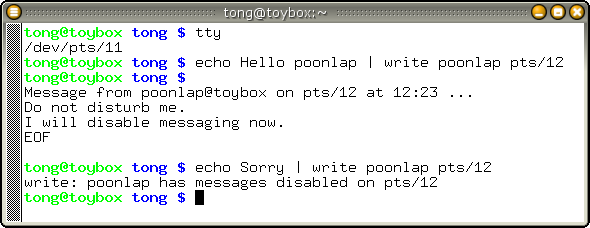
\includegraphics{write_1.eps}}

\vspace{10pt}
\scalebox{.6}{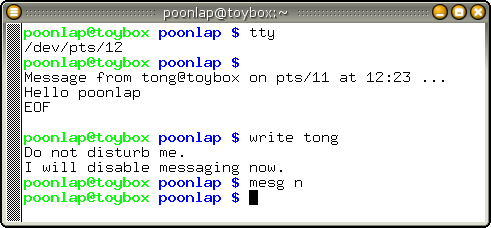
\includegraphics{write_2.eps}}
\caption{ใช้ \cmd{write} ส่งข้อความระหว่างผู้ใช้ในระบบ.}\label{fig:write}
\end{figure}

ในบางกรณีอาจจะมีความจำเป็นต้องส่งข้อความผ่านเทอร์มินอลหาผู้ใช้ทุกคนในระบบที่ใช้เทอร์มินอลอยู่, ให้ใช้คำสั่ง \cmd{wall}\cindex{wall}\refcmd{wall} ส่งข้อมูลให้ผู้ใช้ที่ใช้เทอร์มินอลทุกตัวในระบบ.

\medskip
ปัจจุบัน \emph{Instant Messenger}\gindex{instant messenger} เช่น MSN messenger, Yahoo messenger เป็นเครื่องมือที่นิยมใช้สื่อสารส่งข้อความผ่านทางเน็ตเวิร์ก. ในระบบฏิบัติการแบบยูนิกซ์ช่วงแรกก็มีโปรแกรมแบบนี้เช่นเดียวกันใช้คุยกันผ่านทางเน็ตเวิร์กได้แก่ \cmd{talk}\cindex{talk} หรือ \cmd{phone}\cindex{phone}. โปรแกรม \cmd{talk} จะใช้เทอร์มินอลในการสื่อสารง่ายต่อการใช้. ในปัจจุบันไม่นิยมใช้กันเท่าไหร่นักและในลินุกซ์ก็มีโปรแกรม Instant Messenger ที่เข้ากันได้กับ MSN messenger หรือ Yahoo messenger ด้วย.

\subsubsection{ปรับแต่งเทอร์มินอล}
ถ้าผู้อ่านเคยใช้เทอร์มินอลหลายๆแบบหลายๆที่อาจจะสังเกตุเห็นว่าพฤติกรรมการแสดงผลหรือคีย์บอร์ดที่ใช้บางทีจะไม่เหมือนกัน. สาเหตุหนึ่งคือประเภทของเทอร์มินอลไม่เหมือนกันซึ่งสามารถแก้ได้ด้วยการตั้งค่าตัวแปรสภาพแวดล้อม \cmd{TERM} ให้ถูกต้อง. อีกสาเหตุหนึ่งคือการตั้งค่าเฉพาะของเทอร์มินอลไม่เหมือนกัน. เราสามารถดูค่าของเทอร์มินอลต่างๆที่ตั้งไว้ด้วยคำสั่ง \cmd{stty}\cindex{stty}\refcmd{stty}.

\begin{MyExample}[ดูค่าของเทอร์มินอลๆที่ตั้งไว้.]
\begin{MyEx}
$ \cin{stty -a}
speed 38400 baud; rows 24; columns 80; line = 0;
intr = ^C; quit = ^\bs{}; erase = ^?; kill = ^U; eof = ^D; eol = M-^?; eol2 = M-^?;
start = ^Q; stop = ^S; susp = ^Z; rprnt = ^R; werase = ^W; lnext = ^V;
flush = ^O; min = 1; time = 0;
-parenb -parodd cs8 hupcl -cstopb cread -clocal -crtscts
-ignbrk brkint -ignpar -parmrk -inpck -istrip -inlcr -igncr icrnl ixon -ixoff
-iuclc ixany imaxbel
opost -olcuc -ocrnl onlcr -onocr -onlret -ofill -ofdel nl0 cr0 tab0 bs0 vt0 ff0
isig icanon iexten echo echoe echok -echonl -noflsh -xcase -tostop -echoprt
echoctl echoke
\end{MyEx}
\end{MyExample}%$

จากผลลัพธ์ของคำสั่งจะเห็นว่ามีการกำหนดคีย์ต่างๆให้เข้ากับสัญญาณที่ต้องการเช่นใช้ \cmd{\^{ }C} (กดคีย์ \keyctrl{} ค้างไว้แล้วกดคีย์ \keyc{} ตาม) จะหมายถึงการส่งสัญญาณ Interrupt ให้โปรแกรมเลิกทำงานเป็นต้น. อีกตัวอย่างที่จะแนะนำในที่นี้คือความสามารถ echo. เวลาเรากดคีย์ต่างๆจะเห็นว่าอักษรที่พิมพ์จะปรากฏบนหน้าจอเทอร์มินอล. นี่เป็นความสามารถของเทอร์มินอลที่เรียกว่า echo. 
\begin{MyExample}[หยุดการแสดงผลของสิ่งที่พิมพ์จากแป้นพิมพ์.]
\begin{MyEx}
$ \cin{stty -echo}
$ I can not see \mycomment{พิมพ์ \cmd{echo I can not see} แต่จะไม่แสดงสิ่งที่พิมพ์ไป. จะแสดงแค่ผลลัพธ์.}
$ $ \mycomment{พิมพ์ \cmd{stty echo} เพื่อกลับสู่สภาพปรกติ.}
$ \cin{echo Now I can see again}
Now I can see again
\end{MyEx}
\end{MyExample}%$
การประยุกต์ใช้การตั้งค่าเทอร์มินอลในลักษณะนี้เช่นใช้ในเวลาต้องการให้ผู้ใช้พิมพ์ข้อความที่เป็นความลับ, รหัสผ่าน. ในกรณีนี้สามารถตั้งค่าให้เทอร์มินอลไม่ echo รหัสผ่านที่พิมพ์ทางหน้าจอ. 

คำสั่ง \cmd{stty} ยังสามารถใช้แก้ไขเทอร์มินอลที่มีการแสดงผลไม่ถูกต้องหลังจากที่เปิดดูไฟล์ไบนารี. ในกรณีนี้จะใช้คำสั่ง ``\cmd{stty sane}'' เพื่อปรับสภาพของเทอร์มินอลให้เป็นปรกติ. หรือจะใช้คำสั่ง \cmd{reset} ที่เคยแนะนำไปแล้วก็ได้. 

\medskip
พฤติกรรมของเทอร์มินอลที่สามารถกำหนดได้ด้วยคำสั่ง \cmd{stty} มีหลายอย่างให้อ่านรายละเอียดจาก \cmd{stty(1)}. 

\subsection{ควบคุมคำสั่ง}
ลินุกซ์เป็นระบบปฏิบัติการที่สามารถใช้โปรแกรมหลายโปรแกรมพร้อมๆกัน. ลินุกซ์เคอร์เนลจะมีหน้าที่แบ่งเวลาให้โปรเซสต่างๆใช้หน่วยประมวลผลทำงาน. เราสามารถใช้คำสั่ง \cmd{nice} เปลี่ยนความสำคัญของโปรเซส (scheduling priority) บางตัวที่ไม่สำคัญให้หน่วยประมวลไม่ต้องเสียเวลากับโปรเซสนั้นมากกนัก. ในทางกลับกัน, สามารถกำหนดให้หน่วยประมวลผลใช้เวลากับโปรเซสที่สำคัญมากขึ้นกว่าปรกติได้. คำสั่ง \cmd{nice} มักจะใช้โปรแกรมที่ใช้เวลาทำงานนานๆหรือโปรแกรมที่ทำงานแบบ background. คำสั่งที่ทำงานใช้เวลาไม่มากแล้วจบทันทีไม่จำเป็นต้นใช้ \cmd{nice}.

คำสั่ง \cmd{nice}\cindex{nice}\refcmd{nice} ใช้ตอนที่จะเรียกใช้โปรแกรมที่ต้องการ.\mymemo{สมมติว่าโปรแกรม \cmd{a.out} เป็นโปรแกรมที่เขียนขึ้นเอง.}
\begin{MyExample}[ตั้งความสำคัญของโปรเซสเวลารัน.]
\begin{MyEx}
$ \cin{nice -n 19 ./a.out}
\end{MyEx}
\end{MyExample}%$
ตัวเลือก \cmd{-n} เป็นการระบุความสำคัญ (priority) ของคำสั่งโดยความสำคัญจะเป็นตัวเลขตั้งแต่ -20 จนถึง 19. ค่าตัวเลขยิ่งน้อยยิ่งมีความสำคัญสูง. ถ้าไม่มีการระบุความสำคัญจะถือว่ามีค่าเป็น 10 โดยปริยาย. ผู้ใช้ทั่วไปไม่สามารถใช้ค่าความสำคัญมากได้แก่เลขที่มีค่าน้อยกว่า 0, ต้องเป็น root เท่านั้น.

คำสั่ง \cmd{nice} จะตั้งค่าความสำคัญของโปรเซสได้ตอนที่จะสั่งคำสั่งเท่านั้น. ถ้าต้องการเปลี่ยนความสำคัญของโปรแกรมที่สั่งแล้ว (โปรเซส) จะใช้คำสั่ง \cmd{renice}\cindex{renice}\refcmd{renice} ซึ่ง root เท่านั้นที่จะใช้คำสั่งนี้ได้.
\begin{MyExample}[เปลี่ยนความสำคัญของโปรเซส.]
\begin{MyEx}
# \cin{renice -10 -p 5362}
5362: old priority 0, new priority -10
\end{MyEx}
\end{MyExample}
จากตัวอย่างเป็นการเปลี่ยนค่าความสำคัญของโปรเซสหมายเลข 5362 ให้เป็น -10 (ความสำคัญมากขึ้น). 


 
\medskip
ในบทที่ผ่านมาเราได้ทำความรู้จักกับการสั่งคำสั่งแบบ background ไปแล้ว. สมมติว่าเราล็อกอินผ่านทางเน็ตเวิร์กเพื่อสั่งคำสั่งอะไรบางอย่าง. คำสั่งนั้นกินเวลานานเกินกว่าที่จะรอได้, ในกรณีเราสามารถสั่งคำสั่งแบบ background และล็อกเอาท์ออกจากระบบนั้นโดยไม่ต้องรอให้โปรแกรมที่รันจบแล้วค่อยล็อกเอาท์. คำสั่งที่สั่งจะทำงานต่อไปถึงแม้ว่าเราจะล็อกเอาท์ไปแล้วก็ตามเพราะเราสั่งคำสั่งแบบ background. ถ้าคำสั่งนั้นยกเลิกการทำงานถึงแม้ว่าจะสั่งคำสั่งแบบ background แล้วล็อกเอาท์, ให้ใช้คำสั่ง \cmd{nohup} ช่วย.

%สำหรับเหตุการณ์เดียวกันผู้ใช้อาจจะใช้คำสั่ง \cmd{nohup} ในการสั่งคำสั่งที่กินเวลานานแล้วล็อกเอาท์จากระบบก็ได้. 
การใช้คำสั่ง \cmd{nohup}\cindex{nohup}\refcmd{nohup} ทำได้ดังนี้.
\begin{MyExample}[ให้คำสั่งทำงานต่อไปหลังจากล็อกเอาท์.]
\begin{MyEx}
$ \cin{nohup ./a.out &}
[1] 11599 \mycomment{หมายเลขโปรเซส}
$ \cin{logout} \mycomment{ล็อกเอาท์ได้โดยที่ \cmd{a.out} ทำงานต่อไปเรื่อยๆจนจบ.}
\end{MyEx}
\end{MyExample}
ผู้ใช้ต้องสั่งคำสั่งเป็นแบบ background เอง. หลังจากนั้นสามารถล็อกเอาท์ได้โดยที่คำสั่งนั้นยังคงทำงานต่อไป. ถ้าคำสั่งนั้นมีการส่งข้อมูลออกทาง stdout จะเก็บไว้ในไฟล์ \cmd{nohup.out}. ในทางเทคนิคแล้วคำสั่ง \cmd{nohup} จะทำให้โปรแกรมที่สั่งเพิกเฉยกับสัญญาณ SIGHUP ทำให้ผู้ใช้สามารถล็อกเอาท์ได้. คำสั่ง \cmd{nohup} จะไม่เปลี่ยนความสำคัญของโปรเซสให้, ถ้าต้องการให้คำสั่งนั้นกระทำการโดยมีความสำคัญต่ำให้ใช้คำสั่ง \cmd{nice} เข้าช่วย.


\subsection{นอนพัก}
\cmd{sleep} เป็นคำสั่งที่หยุด, ไม่ทำอะไรตามระยะเวลาที่กำหนด. เช่นถ้าต้องการหยุดรอ 2 นาทีแล้วค่อยสั่งคำสั่งทำได้ดังนี้.
\begin{MyExample}[ใช้คำสั่ง \cmd{sleep}.]
\begin{MyEx}
$ \cin{sleep 2m; echo 'Wake up!'}
Wake up! \mycomment{เวลาผ่านไป 2 นาทีแล้ว \cmd{echo} จึงทำงาน.}
\end{MyEx}
\end{MyExample}%$
ระยะเวลาถ้าเป็นตัวเลขโดยไม่มีหน่วยจะหมายถึงวินาที, m หมายถึงนาที, h หมายถึงชั่วโมง, และ d หมายถึงวัน.

\subsection{คณิตศาสตร์}
คำสั่ง \cmd{expr}\cindex{expr}\refcmd{expr} สามารถใช้คำนวณคณิตศาสตร์ง่ายๆเช่นบวก, ลบ, คูณ, หารได้ตามตัวอย่างต่อไปนี้.
\begin{MyExample}[ใช้ \cmd{expr} คำนวณคณิตศาสตร์แบบง่ายๆ.]
\begin{MyEx}
$ \cin{expr 1 + 2 + 3}
6
$ \cin{expr 1 - 2}
-1
$ \cin{expr 2 \bs{}* 4} \mycomment{ต้องใช้เครื่องหมาย \bs{} นำหน้า \cmd{*}}
8
$ \cin{expr 5 / 3}
1 \mycomment{ปัดเศษทิ้ง}
$ \cin{expr 5 % 3}
2 \mycomment{เศษของการหารด้วย \cmd{3}}
\end{MyEx}
\end{MyExample}%$
การคำนวณนี้สามารถทำได้เฉพาะเลขจำนวนเต็มเท่านั้นและระหว่างตัวปฏิบัติการต้องมีช่องไฟคั่น. คำสั่งนี้ใช่ไม่สะดวกเท่าไหร่นักและสามารถใช้ความสามารถการกระจายนิพจน์คณิตศาสตร์ของเชลล์ bash จะสะดวกกว่า. ตัวอย่างต่อไปนี้จะให้ผลเหมือนตัวอย่างที่แสดงไปแล้วแต่จะใช้ความสามารถของเชลล์ bash แทน.
\begin{MyExample}[ใช้ความสามารถของเชลล์คำนวณคณิตศาสตร์แบบง่ายๆ.]
\begin{MyEx}
$ \cin{echo $((1+2+3))}
6
$ \cin{echo $((1-2))}
-1
$ \cin{echo $((2*4))} \mycomment{ไม่ต้องมีเครื่องหมาย \bs{} นำหน้า \cmd{*}}
8
$ \cin{echo $((5/3))}
1 \mycomment{ปัดเศษทิ้ง}
$ \cin{echo $((5%3))}
2 \mycomment{เศษของการหารด้วย \cmd{3}}
\end{MyEx}
\end{MyExample}

\begin{table}[!htb]
\center
\medskip
\caption{ตัวปฏิบัติการคณิตศาสตร์ต่างๆที่ใช้ในเชลล์.}\label{tab:shellop}
\begin{tabular}{lp{.7\textwidth}}
\toprule
\multicolumn{1}{c}{ตัวปฏิบัติการ} & \multicolumn{1}{c}{ความหมาย}\\
\midrule
\cmd{\textit{var}++} \cmd{\textit{var}--} & เพิ่มหรือลดค่าของตัวแปรหลังใช้งาน.\\
\cmd{++\textit{var}} \cmd{--\textit{var}} & เพิ่มหรือลดค่าของตัวแปรก่อนใช้งาน.\\
\cmd{! \~} & ตัวกระทำเชิงตรรกะให้เป็นเท็จ. หรือกลับค่าบิต.\\
\cmd{**} & ยกกำลัง.\\
\cmd{+ - * /} & บวก, ลบ, คูณ, หาร.\\
\cmd{\%} & เศษของการหาร.\\
\cmd{<< >>} & เลื่อนบิตไปทางซ้ายหรือขวา.\\
\cmd{<= >= < > != ==} & เปรียบเทียบค่า.\\
\cmd{\&} & ตัวปฏิบัติการบิต AND.\\
\cmd{\^} & ตัวปฏิบัติการบิต exclusive OR.\\
\cmd{|} & ตัวปฏิบัติการบิต OR.\\
\cmd{\&\&} & ตัวปฏิบัติการตรรกะ AND.\\
\cmd{||} & ตัวปฏิบัติการตรรกะ OR.\\
\bottomrule
\end{tabular}
\end{table}


\medskip
คำสั่ง \cmd{factor}\cindex{factor}\refcmd{factor} จะแสดงตัวประกอบของเลขจะนวนเต็มที่เป็นอาร์กิวเมนต์.
\begin{MyExample}[หาตัวประกอบของจำนวนที่ต้องการ.]
\begin{MyEx}
$ \cin{factor 20 9 2004 23354523}
20: 2 2 5
9: 3 3
2004: 2 2 3 167
23354523: 3 3 2594947
\end{MyEx}
\end{MyExample}%$
เนื่องจากตัวประกอบของเลขจำนวนเฉพาะ (prime) คือตัวมันเอง. ดังนั้นเราสามารถใช้คำสั่ง \cmd{factor} ตรวจสอบจำนวนที่ต้องการว่าเป็นจำนวนเฉพาะหรือไม่ได้.

\medskip
คำสั่งที่เกี่ยวข้องกับคณิตศาสตร์อันสุดท้ายคือ \cmd{seq} และมีประโยชน์ใช้ในการเขียนเชลล์สคริปต์ด้วย. คำสั่ง \cmd{seq}\cindex{seq}\refcmd{seq} จะแสดงจำนวนตัวเลขเป็นลำดับไปเรื่อยๆตัวอย่างเช่น.
\begin{MyExample}[แสดงลำดับของจำนวนไปเรื่อยๆ.]
\begin{MyEx}
$ \cin{seq 3} \mycomment{ถ้ามีอาร์กิวเมนต์ตัวเดียวจะเริ่มตั้งแต่ \cmd{1}}
1
2
3
$ \cin{seq -s ' ' 10 19} \mycomment{ลำดับเพิ่มทีละ \cmd{1} ตั้งแต่ \cmd{10} ถึง \cmd{19}}
10 11 12 13 14 15 16 17 18 19
$ \cin{seq -s ' ' -w 5 5 50} \mycomment{ลำดับเพิ่มทีละ \cmd{5} ตั้งแต่ \cmd{5} ถึง \cmd{50}}
05 10 15 20 25 30 35 40 45 50
\end{MyEx}
\end{MyExample}%$
ตัวเลือก \cmd{-s} ใช้ระบุสายอักขระที่ต้องการใช้เป็นตัวคั่นระหว่างจำนวน. ถ้าไม่ระบุจะใช้ \cmd{\bs{}n} เป็นตัวคั่นระหว่างจำนวนโดยปริยาย. ตัวเลือก \cmd{-w} จะเติมเลข 0 ก่อนหน้าตัวเลขทำให้จำนวนที่แสดงทั้งหมดมีขนาดเท่ากัน (ใช้จำนวนตัวอักษรเท่ากัน). คำสั่ง \cmd{seq} นี้มีประโยชน์ใช้ในเชลล์สคริปต์ร่วมกับไวยกรณ์ \cmd{for}.
\begin{MyExample}[ใช้ \cmd{seq} ร่วมกับ \cmd{for}]
\begin{MyEx}
$ \cin{for i in `seq -f '%03g' 10`} \mycomment{ใช้ตัวเลือก \cmd{-f} จัดรูปแบบจำนวน}
> \cin{do}
> \cin{wget -nd http://somewhere.net/doc/$i.html} \mycomment{ใช้โปรแกรมคำสั่ง \cmd{wget} ดาว์นโหลดไฟล์}
> \cin{done}
\end{MyEx}
\end{MyExample}
ตัวอย่างข้างบนเป็นการใช้คำสั่ง \cmd{seq} ร่วมกับไวยกรณ์ \cmd{for} เพื่อดาว์นโหลดเอกสารที่เป็นตัวเลขเรียงกันเช่น \cmd{001.html}, \cmd{002.html} ฯลฯ ด้วยคำสั่ง \cmd{wget}. ในตัวอย่างจะใช้ตัวเลือก \cmd{-f} เพื่อระบุรูปแบบที่ต้องการคือให้เติมศูนย์ให้จำนวนเต็มมีขนาด 3 ตัวอักษร.

\subsection{ซ้ำ}
\cmd{yes}\cindex{yes}\refcmd{yes} เป็นคำสั่งที่แปลกคือจะแสดงตัวอักษร \cmd{y} ไปเรื่อยๆบรรทัดต่อบรรทัดจนกว่าจะกด \cmd{C-c} เพื่อหยุดการทำงาน. ถ้าให้อากิวเมนต์เป็นคำว่า Hello ก็จะแสดงคำว่า Hello ไปเรื่อยๆ. คำสั่งนี้สามารถใช้ร่วมกับคำสั่งอื่นที่ต้องการคำตอบและผู้ใช้ขี้เกียจพิมพ์ \cmd{y} (หรือสายอักขระใดๆก็ได้) ไปเรื่อยๆเพื่อตอบคำถาม. ตัวอย่างเช่นคำสั่งที่ใช้ลบไฟล์ \cmd{rm -i} จะถามย้ำให้เราตอบ \cmd{y} หรือ \cmd{n} ทุกครั้งที่จะลบไฟล์. แทนที่เราต้องพิมพ์ \cmd{y} ตอบด้วยมือ, สามารถทำตามตัวอย่างต่อไปนี้ได้. 
\begin{MyExample}[ใช้คำสั่ง \cmd{yes} ตอบคำถามที่ซ้ำๆกัน.]
\begin{MyEx}
$ \cin{yes | rm *} \mycomment{สมมติว่า \cmd{rm} คือ alias ของ \cmd{rm -i}}
\end{MyEx}
\end{MyExample}%$


\subsection{เปลี่ยนตัวเองเป็นผู้ใช้อื่น}
คำสั่ง \cmd{su} ใช้สำหรับเปลี่ยน ID จากผู้ใช้คนหนึ่งไปเป็นผู้ใช้ที่ต้องการ. โดยปรกติจะมักใช้เปลี่ยน ID ของผู้ใช้ทั่วไปเป็น root เพื่อสั่งคำสั่งที่ผู้ใช้ทั่วไปไม่สามารถสั่งได้. นอกจากการเปลี่ยน ID ของผู้ใช้แล้วยังสามารถใช้คำสั่ง \cmd{su} สั่งคำสั่งที่ต้องการโดยใช้ ID ของคนอื่นเป็นผู้กระทำได้ด้วยโดยที่ไม่ต้องเปลี่ยน ID เป็นคนนั้น. 

\begin{MyExample}[ใช้ \cmd{su} สั่งคำสั่งด้วย ID ของคนอื่น.]
\begin{MyEx}
$ \cin{su -c "cat /etc/shadow"}
Password: \mycomment{ใส่พาสเวิร์ดของ root}
...
halt:*:9797:0:::::
operator:*:9797:0:::::
shutdown:*:9797:0:::::
...
\end{MyEx}
\end{MyExample}%$
เนื่องจาก ID ที่ใช้สั่งคำสั่ง \cmd{cat} คือ root, จึงสามารถเปิดอ่านไฟล์ที่ root ดูได้แต่คนอื่นอ่านไม่ได้เช่นไฟล์ \cmd{/etc/shadow} เป็นต้น. การที่เปลี่ยน ID ในลักษณะนี้เรียกว่า \emph{effective user ID}\gindex{effective user ID} คือ ID ที่มีผลจริงขณะปฏิบัติงาน. 

%\cmd{su} เป็นคำสั่งที่คำสั่งที่อนุญาติให้คนใดคนหนึ่งเปลี่ยน ID เป็นอีกคนหนึ่ง, หรือสั่งคำสั่งด้วย ID ของใครก็ได้. แต่วิธีนี้ยังไม่สะดวกเท่าไรนักเพราะผู้ใช้คำสั่งต้องรู้รหัสผ่านของ ID ที่ต้องการเปลี่ยน\mymemo{ถ้า root เป็นครใช้คำสั่ง \cmd{su} ไม่จำเป็นต้องรู้รหัสผ่านของ ID ที่ต้องการเปลี่ยน.}. ดังนั้นในระบบใหม่ๆจึงมีคำสั่งที่คล้ายๆกันคือ \cmd{sudo}. คำสั่ง \cmd{sudo} เป็นคำสั่งที่อนุญาติให้ผู้ใช้ที่ระบุในไฟล์ \cmd{sudoers}

\section{แพ็กเกจ textutils}
จุดเด่นของคำสั่งในระบบปฏิบัติการยูนิกซ์ซึ่งสืบทอดมาถึงลินุกซ์ได้แก่คำสั่งที่ใช้จัดการไฟล์เท็กซ์ทั้งหลาย. เนื่องจากคำสั่งเหล่านี้รับข้อมูลเป็นเท็กซ์และให้ผลลัพธ์เป็นเท็กซ์, การใช้คำสั่งต่างๆร่วมกันโดยใช้ไปป์จึงสะดวกและมีประสิทธิภาพในหลายๆด้าน. ในช่วงนี้จะแนะนำคำสั่งที่ประมวลผลข้อมูลเท็กซ์ซึ่งจะมีประโยชน์ไม่ว่าจะใช้ช่วยการพัฒนาซอฟต์แวร์, ดูและระบบ, หรือใช้งานทั่วไป. 


\begin{longtable}{lp{.55\textwidth}l}
\caption{โปรแกรมคำสั่งในแพ็กเกจ textutils.}\label{tab:textutils}\\
\toprule
\multicolumn{1}{c}{คำสั่ง} & \multicolumn{1}{c}{คำอธิบาย} & \multicolumn{1}{c}{อ้างอิง}\\
\midrule
\cmd{cat} & รวมข้อมูลแล้วแสดงผลทาง stdout.& หน้า \pageref{cmd:cat}\\
\cmd{cksum} & แสดงผลรวมตรวสอบ (checksum) และนับจำนวนไบต์ในไฟล์.& หน้า \pageref{cmd:cksum}\\
\cmd{comm} & เปรียบเทียบไฟล์สองไฟล์บรรทัดต่อบรรทัด.& หน้า \pageref{cmd:comm}\\
\cmd{csplit} & แยกไฟล์ออกเป็นไฟล์ย่อยๆตามเนื้อหาที่ระบุ.&\\
\cmd{cut} & ตัดส่วนที่ไม่ต้องการออกจากทุกบรรทัดในไฟล์.& หน้า \pageref{cmd:cut}\\
\cmd{expand} & เปลี่ยน tab ให้เป็น space.& หน้า \pageref{cmd:expand}\\
\cmd{fmt} & จัดรูปแบบของข้อความให้เหมาะสม.&\\
\cmd{fold} & ตัดบรรทัดของข้อมูลเข้าตามความกว้างที่ระบุ.&\\
\cmd{join} & รวมบรรทัดของไฟล์สองไฟล์เมื่อเจอส่วนที่เหมือนกัน.& หน้า \pageref{cmd:join}\\
\cmd{md5sum} & คำนวณและตรวจสอบค่า MD5.& หน้า \pageref{cmd:md5sum}\\
\cmd{nl} & แสดงเลขบรรทัดของไฟล์ที่ต้องการ.& หน้า \pageref{cmd:nl}\\
\cmd{od} & เทข้อมูล (dump) ออกมาให้อยู่ในรูปแบบเลขฐานแปดและอื่นๆ.& หน้า \pageref{cmd:od}\\
\cmd{paste} & นำข้อมูลในไฟล์เป็นบล็อกมาต่อกันในแนวนอน.& หน้า \pageref{cmd:paste}\\
\cmd{pr} & แปลงข้อความในไฟล์เพื่อพิมพ์ออกทางเครื่องพิมพ์.&\\
\cmd{ptx} & สร้าง permuted index.&\\
\cmd{sort} & เรียงลำดับบรรทัดในไฟล์.& หน้า \pageref{cmd:sort}\\
\cmd{split} & แบ่งไฟล์ออกเป็นไฟล์ย่อยๆ.& หน้า \pageref{cmd:split}\\
\cmd{sum} & คำนวณผลรวมตรวจสอบ (checksum) และนับบล็อก.&\\
\cmd{tac} & รวมไฟล์และแสดงผลแบบกลับบรรทัด (ตรงข้ามกับ \cmd{cat})&\\
\cmd{tail} & แสดงช่วงท้ายของไฟล์.& หน้า \pageref{cmd:tail}\\
\cmd{tr} & แปลงและลบอักขระที่ต้องการ.& หน้า \pageref{cmd:tr}\\
\cmd{tsort} & จัดลำดับ topological sort.&\\
\cmd{unexpand} & เปลี่ยน space เป็น tab.& หน้า \cmd{unexpand}\\
\cmd{uniq} & ลบบรรทัดที่ซ้ำกัน. มักใช้ร่วมกับคำสั่ง \cmd{sort}.& หน้า \pageref{cmd:uniq}\\
\cmd{wc} & แสดงจำนวนไบต์, คำ, และบรรทัดในไฟล์.& หน้า \pageref{cmd:wc}\\
\cmd{head} & แสดงส่วนต้นๆของไฟล์.& หน้า \pageref{cmd:head}\\
\bottomrule
\end{longtable}

\subsection{แสดงข้อมูล}
\begin{figure}[!htb]
\plfigure{.8}{file_display.eps}{คำสั่งที่ใช้แสดงข้อมูลส่วนต่างๆ.}{file_display}
\end{figure}

จากบทที่ผ่านมามีตัวอย่างการใช้งานคำสั่ง \cmd{cat} มากพอและไม่จำเป็นต้องอธิบายแล้วว่าคำสั่ง \cmd{cat} ใช้ทำอะไร. คำสั่ง \cmd{cat} สามารถใช้แสดงเลขบรรทัดทุกบรรทัดด้วยตัวเลือก \cmd{-n} ซึ่งในแพ็กเกจ textutils ก็มีคำสั่งที่ใช้เลขบรรทัดในไฟล์ด้วยเหมือนกันแต่มีลูกเล่นมากกว่า.

ถ้าใช้คำสั่ง \cmd{nl}\cindex{nl}\refcmd{nl} โดยไม่มีอาร์กิวเมนต์จะแสดงเลขบรรทัดเฉพาะบรรทัดที่มีข้อมูลเท่านั้น. คำสั่ง \cmd{nl} สามารถแสดงเลขบรรทัดได้หลายแบบขึ้นอยู่กับตัวเลือกที่ระบุ. การแสดงเลขบรรทัดที่คำสั่ง \cmd{cat} ไม่สามารถทำได้เช่นการเติมศูนย์ที่ตัวเลขให้มีจำนวนตัวอักษรเท่ากัน.

\begin{MyExample}[ใช้ \cmd{nl} แสดงเลขบรรทัด.]
\begin{MyEx}
$ \cin{yes | head -n 5 | nl -n rz -b a -w 3} \mycomment{ใช้คำสั่ง \cmd{yes} สร้างข้อมูล 5 บรรทัด}
001     y
002     y
003     y
004     y
005     y
\end{MyEx}
\end{MyExample}%$

จากตัวอย่างเป็นการแสดงเลขบรรทัดโดยจัดให้เลขบรรทัดชิดขวาและเติมเลขศูนย์ด้วยตัวเลือก \cmd{-n rz}, แสดงตัวเลขทุกบรรทัดด้วยตัวเลือก \cmd{-b a} และให้เลขบรรทัดมีสามหลักด้วยตัวเลือก \cmd{-w 3}. คำสั่ง \cmd{nl} จะมีประโยชน์เมื่อต้องการดูเลขบรรทัดเช่นเวลาพิมพ์รหัสต้นฉบับพร้อมเลขบรรทัดออกทางเครื่องพิมพ์.

\medskip
คำสั่ง \cmd{tac}\cindex{tac} เป็นการเล่นคำโดยกลับตัวอักษรของคำสั่ง \cmd{cat} เป็น \cmd{tac}. คำสั่งนี้จะแสดงข้อมูลเป็นบรรทัดโดยจะแสดงข้อมูลที่อยู่ในบรรทัดสุดท้ายก่อนไล่ขึ้นไปเรื่อยๆจนถึงบรรทัดแรกซึ่งการทำงานนี้จะตรงกันข้ามกับคำสั่ง \cmd{cat}. นอกจากนี้ยังมีคำสั่ง \cmd{rev}\cindex{rev} สำหรับแสดงข้อมูลจากข้างหลังไปข้างหน้า, ไบต์ต่อไบต์.

\subsection{จัดรูปแบบข้อมูล}
คำสั่งที่ใช้จัดรูปแบบข้อมูลเท็กซ์ได้แก่ \cmd{fmt}, \cmd{pr} และ \cmd{fold}. คำสั่งเหล่านี้สร้างมาเพื่อใช้กับข้อมูลเท็กซ์ภาษาอังกฤษแต่ก็ควรจะรู้ไว้เพราะเป็นคำสั่งที่ใช้งานได้จริงและมีประโยชน์. 

รูปที่ \ref{fig:fmt} แสดงความแตกต่างระหว่างข้อมูลเท็กซ์ที่ยังไม่ได้จัดย่อหน้ากับข้อมูลที่จัดย่อหน้าแล้วด้วยคำสั่ง \cmd{fmt}.

\begin{figure}[!htb]
\ifthenelse{\isodd{\pageref{fig:fmt}}}%
{\parbox{\headwidth}{\center\scalebox{.35}{
\includegraphics{fmt_1.eps}~~~~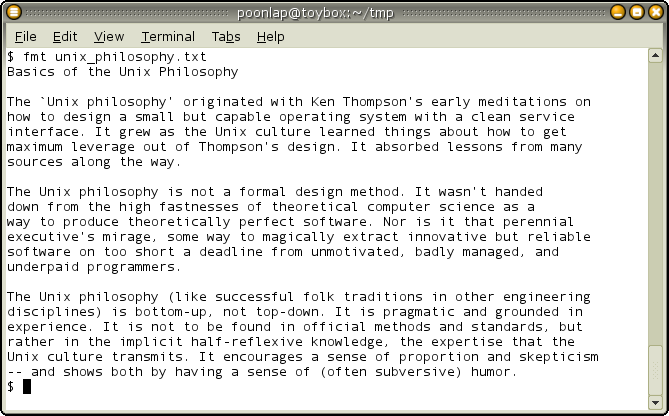
\includegraphics{fmt_2.eps}}\caption{ใช้ \cmd{fmt} จัดรูปแบบข้อมูล.}\label{fig:fmt}}}%
{\leftskip=\moveback\parbox{\headwidth}{\center\scalebox{.35}{
\includegraphics{fmt_1.eps}~~~~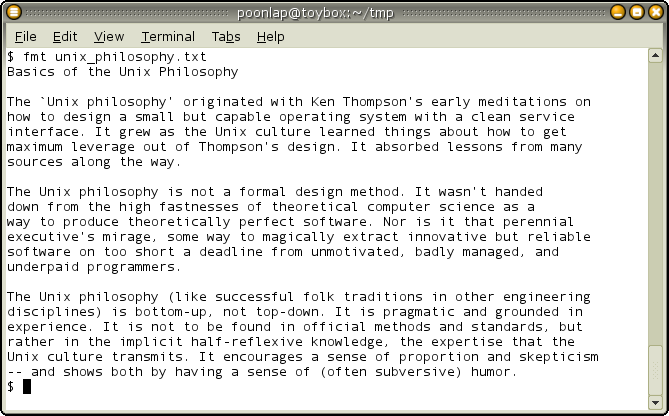
\includegraphics{fmt_2.eps}}\caption{ใช้ \cmd{fmt} จัดรูปแบบข้อมูล.}\label{fig:fmt}}}
\end{figure}

คำสั่ง \cmd{fmt}\cindex{fmt}\refcmd{fmt} จะพยายามตัดเรียงข้อมูลเป็นบรรทัดๆ โดยที่แต่ละบรรทัดมีความยาวไม่เกิน 75 ตัวอักษร. จำนวนอักษรนี้สามารถกำหนดได้ด้วยตัวเลือก \cmd{-w} (width). ถ้าใช้ตัวเลือก \cmd{-u} จะเป็นการลบช่องไฟที่เกินและไม่จำเป็นได้ด้วย. ตัวอย่างเช่น ``a\ \ pencil'' เป็น ``a pencil''. บรรทัดว่างที่อยู่ในข้อมูลนำเข้าจะถือว่าเป็นการเริ่มต้นย่อหน้า. คำสั่ง \cmd{fmt} จะแบ่งบรรทัดที่ยาวเกินจำนวนอักษรที่กำหนดและจะรวมบรรทัดที่สั้นๆให้มีความกว้างไม่เกินที่กำหนด. 

\medskip
คำสั่ง \cmd{pr}\cindex{pr} ใช้สำหรับจัดเรียงหน้าเพื่อพิมพ์ออกทางเครื่องพิมพ์. การจัดเรียงหน้านี้เป็นการจัดเรียงแบบง่ายๆตามความกว้างของบรรทัด (72 ตัวอักษร) และความยาวของหน้าในหน่วยบรรทัด (66 บรรทัด). นอกจากนี้คำสั่ง \cmd{fmt} จะพิมพ์หัวกระดาษให้ด้วย. 

\begin{figure}[!tb]
\plfigure{.35}{pr.eps}{ใช้คำสั่ง \cmd{fmt} และ \cmd{pr} จัดหน้ากระดาษแบบง่ายๆ.}{pr}
\end{figure}

คำสั่งสุดท้ายที่ใช้จัดข้อมูลคือ \cmd{fold}\cindex{fold}. คำสั่ง \cmd{fold} จะตัดบรรทัดที่ยาวๆให้มีความกว้าง (ตัวอักษร) ไม่เกินความกว้างที่กำหนด. คำสั่งนี้จะคล้ายกับคำสั่ง \cmd{fmt} แต่จะไม่มีการรวมบรรทัดที่ติดกัน. การตัดบรรทัดของคำสั่ง \cmd{fold} จะตัดตามจำนวนอักษรไม่ได้ตัดแบ่งบรรทัดตามช่องว่างทำให้ไม่สวยงาม. ถ้าต้องการตัดบรรทัดด้วยช่องว่าง, คือตัดบรรทัดแบ่งตามคำภาษาอังกฤษให้ใช้ตัดเลือก \cmd{-s}.


\subsection{หัวหาง}
คำสั่งที่ใช้แสดงบางส่วนของไฟล์ในแพ็กเกจ textutils ได้แก่ \cmd{head} และ \cmd{tail}. คำสั่ง \cmd{head} ใช้แสดงส่วนต้นของไฟล์เป็นบรรทัด, ในทางตรงกันข้ามคำสั่ง \cmd{tail} ใช้แสดงส่วนท้ายของไฟล์เป็นบรรทัด.

เราสามารถกำหนดจำนวนบรรทัดที่ต้องการให้แสดงได้ด้วยตัวเลือก \cmd{-n} แล้วตามด้วยจำนวนบรรทัดที่ต้องการ. ตัวเลือกนี้ใช้ได้ทั้งคำสั่ง \cmd{head} และ \cmd{tail}. คำสั่ง \cmd{tail}\cindex{tail} มีประโยชน์ใช้ดู \emph{log}\gindex{log@log file} ของ \emph{daemon} %
\myvocab{d}{daemon}{โปรเซสแบบ background ที่มีโปรเซส ID แม่ (PPID) เป็น 1 (โปรเซส \cmd{init}). โปรเซสเหล่านี้มักจะเป็นโปรเซสที่ทำงานโดยอัตโนมัติถูกสร้างตอนที่ระบบเริ่มทำงาน. โปรเซสเหล่านี้บางตัวอาจเป็นโปรเซสที่ช่วยดูแลระบบ, เซิฟร์เวอร์ เช่น \cmd{cron}, \cmd{sendmail} เป็นต้น.}%
ซึ่ง daemon จะเขียนข้อความลงในไฟล์ล็อกต่อท้ายไฟล์เรื่อยๆถ้ามีเหตุการณ์สำคัญเกิดขึ้น. เราสามารถดูการทำงาน, ข้อผิดพลาดของ deamon ได้จาก log. ตัวอย่างเช่น log เก็บข้อผิดพลาดของเว็บเซิฟร์เวอร์ apache ได้แก่ไฟล์ \cmd{/var/log/apache/error\_log}\mymemo{ไฟล์ log ของ apache อาจจะแตกต่างกันแล้วแต่ระบบและดิสทริบิว, ตลอดจนรุ่นของ apache ที่ใช้.} เราสามารถติดตามดูข้อความที่เขียนในไฟล์นี้ได้เรื่อยโดยใช้ตัวเลือก \cmd{-f}\mymemo{\cmd{-f} ย่อมาจาก follow.}.
\begin{MyExample}[ใช้ \cmd{tail} ติดตามดู log.]
\begin{MyEx}
# \cin{tail -f /var/log/apache/error_log}
[Thu Aug 05 01:53:49 2004] [notice] caught SIGTERM, shutting down
[Thu Aug 05 23:02:43 2004] [notice] Digest: generating secret for digest aut
hentication ...
[Thu Aug 05 23:02:43 2004] [notice] Digest: done
[Thu Aug 05 23:02:44 2004] [notice] Apache/2.0.50 (Gentoo/Linux) configured -- r
esuming normal operations
[Thu Aug 05 23:32:58 2004] [error] [client 219.178.56.123] File does not exist: 
/var/www/localhost/htdocs/default.ida
[Fri Aug 06 00:46:18 2004] [error] [client 219.154.229.60] request failed: URI t
oo long (longer than 8190)
[Fri Aug 06 02:17:14 2004] [notice] caught SIGTERM, shutting down
[Tue Sep 28 21:38:46 2004] [notice] Digest: generating secret for digest authent
ication ...
[Tue Sep 28 21:38:46 2004] [notice] Digest: done
[Tue Sep 28 21:38:47 2004] [notice] Apache/2.0.50 (Gentoo/Linux) configured -- r
esuming normal operations
\cursorprompt \mycomment{คำสั่งทำงานแบบ foreground}
\end{MyEx}
\end{MyExample}
จากตัวอย่างถ้าเซิฟร์เวอร์มีข้อความ notice, error เพิ่มเติมก็จะเขียนใส่ไฟล์ log เพิ่มและ \cmd{tail} ก็จะแสดงบรรทัดที่เขียนเพิ่มเข้ามาโดยอัตโนมัติ. เราอาจจะสั่งคำสั่งแบบ background ก็ได้, แล้วใช้เทอร์มินอลนั้นทำงานอื่นๆต่อไป. ถ้ามีข้อความเพิ่มเติมเข้ามาใน log ก็จะปรากฏในเทอร์มินอลนั้น. การใช้งานแบบนี้เหมาะสำหรับหาสาเหตุ, ข้อผิดพลาดเวลาเซิฟร์เวอร์หรือโปรแกรมที่มีไฟล์ log ทำงานผิดพลาดและเรากำลังแก้ไขอยู่.

บางครั้งถ้าใช้คำสั่ง \cmd{tail} กับตัวเลือก \cmd{-f} ดู log ค้างไว้นาน, มีโอกาสที่ระบบจะเปลี่ยนล็อกไฟล์ที่กำลังดูอยู่ไปเป็นชื่ออื่นแล้วสร้าง log ตัวใหม่ด้วยชื่อเดียวกัน. ตัวอย่างเช่นระบบอาจจะเปลี่ยนชื่อไฟล์ \cmd{error\_log} ไปเป็น \cmd{error\_log.1} แล้วสร้าง log ใหม่ด้วยชื่อ \cmd{error\_log} เหมือนเดิม. สำหรับ log ที่เก่าเกินไปก็อาจจะถูกลบทิ้งไปเพื่อประหยัดพื้นที่. ในกรณีที่มีการเปลี่ยน log แบบนี้คำสั่ง \cmd{tail} กับตัวเลือก \cmd{-f} จะไม่สามารถดู log ที่สร้างใหม่ได้ถึงแม้ว่าจะเป็นชื่อเดียวกันเพราะคำสั่ง \cmd{tail} จะยึดกับ file description เป็นหลัก, ไม่ได้ดูที่ชื่อ. ถ้าต้องการดูไฟล์ที่มีชื่อเดียวกันต่อไปเรื่อยๆต้องใช้ตัวเลือก \cmd{--follow=name} แทน.

\subsection{แบ่งไฟล์, รวมไฟล์}
ในปัจจุบันอาจจะไม่มีความจำเป็นแบ่งไฟล์ที่มีขนาดใหญ่ให้เป็นไฟล์เล็กๆเท่าไรนัก, เพราะมีอุปกรณ์พกพาเก็บข้อมูลขนาดใหญ่เช่นฮาร์ดดิสก์พกพาแบบ USB เป็นต้น. อย่างไรก็ตามผู้อ่านก็ควรจะรู้วิธีการแบ่งไฟล์ให้เป็นไฟล์ย่อยด้วยสำหรับกรณีจำเป็นเช่น การแบ่งไฟล์ขนาดใหญ่ให้เป็นไฟล์ขนาดเล็กหลายๆไฟล์เก็บลงฟล็อปปี้ดิสก์.

การแบ่งไฟล์เป็นไฟล์ย่อยๆสามารถใช้คำสั่ง \cmd{split}\cindex{split}\refcmd{split}. ตัวอย่างเช่นการแบ่งไฟล์ใหญ่ๆให้เป็นไฟล์ย่อยๆมีขนาดพอดีกับฟล็อปปี้ดิสก์ 1440MB ทำได้ดังนี้.

\begin{MyExample}[แบ่งไฟล์ใหญ่ๆให้มีขนาดพอกับแผ่นฟล็อปปี้ดิสก์.]
\begin{MyEx}
$ \cin{split -b `bc <<<'1440*1024'` bigfile small}
$ \cin{ls -l}
total 4108
-rw-r--r--    1 poonlap  users     2097152 Sep 22 23:19 bigfile
-rw-r--r--    1 poonlap  users     1474560 Sep 22 23:24 smallaa
-rw-r--r--    1 poonlap  users      622592 Sep 22 23:24 smallab
\end{MyEx}
\end{MyExample}
ตัวเลือก \cmd{-b} จะแบ่งไฟล์แต่ละไฟล์ให้มีขนาดตามที่กำหนด (ถ้าเป็นไปได้). ในกรณีจะพยายามแบ่งไฟล์ให้มีขนาดเป็น $1440 \times 1024 = 1474560$ ไบต์. การกำหนดจำนวนไบต์ในตัวอย่างใช้การแทนค่าคำสั่ง \cmd{bc} ซึ่งจะคำนวณผลลัพธ์เป็นไบต์ให้. ในตัวอย่างมีการกำหนดชื่อนำหน้าไฟล์ย่อย (prefix) เป็น small. ไฟล์ย่อยที่แบ่งแล้วจะเป็น smallaa และ smallab. aa และ ab คือส่วนตามหลังไฟล์ (suffix) ซึ่งจะเป็นตัวอักษร 2 ตัว. ถ้าต้องการเป็นตัวเลขแทนให้ใช้ตัวเลือก \cmd{-d}.

\medskip
การรวมไฟล์ย่อยๆให้เป็นไฟล์เดียวกันให้ใช้คำสั่ง \cmd{cat}\cindex{cat}.
\begin{MyExample}[รวมไฟล์หลายๆไฟล์ให้เป็นไฟล์เดียวกัน.]
\begin{MyEx}
$ \cin{cat small* > combine} \mycomment{เขียนชื่อไฟล์ \cmd{small*} ได้เพราะเรียงลำดับอยู่แล้ว (\cmd{aa, ab})}
$ \cin{ls -l}
total 6160
-rw-r--r--    1 poonlap  users     2097152 Sep 22 23:19 bigfile
-rw-r--r--    1 poonlap  users     2097152 Sep 22 23:59 combine
-rw-r--r--    1 poonlap  users     1474560 Sep 22 23:58 smallaa
-rw-r--r--    1 poonlap  users      622592 Sep 22 23:58 smallab
\end{MyEx}
\end{MyExample}
เราสามารถตรวจสอบจำนวนไบต์ของไฟล์ที่รวมแล้วโดยใช้คำสั่ง \cmd{ls}. แต่การดูจำนวนไบต์เป็นเพียงแค่การตรวจดูขนาด, ไม่สามารถบอกได้ว่าเนื้อหานั้นถูกต้องหรือไม่. สำหรับการตรวจสอบเนื้อหานั้นอาจจะใช้คำสั่ง \cmd{cksum}\cindex{cksum}\refcmd{cksum} หรือ \cmd{md5sum}\cindex{md5sum}\refcmd{md5sum}.

\begin{MyExample}[ตรวจสอบดูค่าเฉพาะของไฟล์.]
\begin{MyEx}
$ \cin{cksum bigfile combine}
1742489887 2097152 bigfile
1742489887 2097152 combine
$ \cin{md5sum bigfile combine}
b2d1236c286a3c0704224fe4105eca49  bigfile
b2d1236c286a3c0704224fe4105eca49  combine
\end{MyEx}
\end{MyExample}

คำสั่งทั้งสองจะหาค่า \emph{checksum}\mymemo{คำสั่ง \cmd{sum} ก็ใช้หาค่า checksum เช่นกันแต่ไม่ให้ผลไม่ค่อยดีนัก (จำนวนบิตที่ใช้คำนวณน้อย).} %
\myvocab{c}{checksum}{วีธีการตรวจสอบความผิดพลาดของข้อมูล, หรือค่าที่ได้จากการตรวจสอบ. ค่าเหล่านี้สามารถบอกได้ว่าข้อมูลที่ได้รับเช่นข้อมูลผ่านทางเน็ตเวิร์กมีข้อผิดพลาดหรือไม่. วิธีการคำนวณและหาค่าเหล่านี้มีหลายวิธีเช่น cyclic redundancy checks, cryptographic message digest. วิธีแบบ cryptographic message digest ยังมีหลายวิธีเช่น MD5 เป็นต้น. }%
ของข้อมูลแต่ใช้วิธีการคำนวณต่างกัน. ปัจจุบัน \cmd{md5sum} ใช้ในการตรวจสอบไฟล์อิมเมจของซีดีว่าข้อมูลที่ดาว์นโหลดมานั้นถูกต้องหรือไม่, โดยจะมีไฟล์ที่ชื่อ MD5SUMS\mymemo{จริงๆแล้วไฟล์ MD5SUMS จะเป็นชื่ออะไรก็ได้.} อยู่ที่เดียวกันกับไฟล์ที่ดาว์นโหลดด้วย. ในไฟล์นี้จะมีผลลัพธ์ของคำสั่ง \cmd{md5sum} บันทึกอยู่. คนที่ดาว์นโหลดไฟล์ที่ต้องการใช้ให้ใช้คำสั่ง \cmd{md5sum} หาค่า checksum ของไฟล์นั้นแล้วดูเปรียบเทียบกับไฟล์ที่มีค่า checksum ไว้ให้แล้วด้วยตา. หรือจะดาว์นโหลดไฟล์ MD5SUMS มาด้วยแล้วใช้ตัวเลือก \cmd{-c} ตรวจสอบว่าค่า checksum ตรงกันหรือไม่.

\begin{MyExample}[ใช้ \cmd{md5sum} ตรวจสอบความถูกต้องของไฟล์ที่ดาว์นโหลด.]
\begin{MyEx}
$ \cin{ls -l sarge-i386-netinst.iso MD5SUMS}
-rw-r--r--    1 poonlap  users          57 Sep 23 23:25 MD5SUMS
-rw-------    1 poonlap  users    119470080 Sep 12 15:16 sarge-i386-netinst.iso
$ \cin{cat MD5SUMS}
1068812b8de80f05c55119b0dc64e488  sarge-i386-netinst.iso
$ \cin{md5sum -c MD5SUMS}
sarge-i386-netinst.iso: OK
\end{MyEx}
\end{MyExample}%$

\subsection{จัดการข้อมูลที่แบ่งเป็นคอลัมน์}
ในระบบปฏิบัติการลินุกซ์มักใช้ไฟล์เท็กซ์เก็บข้อมูลต่างๆเช่น ไฟล์ \cmd{/etc/shadow}, \cmd{/etc/services} เป็นต้น. ไฟล์เหล่านี้อาจจะเป็นไฟล์ที่เก็บข้อมูลของระบบ, ไฟล์ตั้งค่าเริ่มต้นของโปรแกรม, หรือไฟล์ล็อก (log file) เก็บบันทึกรายงานการทำงานของโปรแกรม ฯลฯ. บางครั้งเราต้องการสกัดข้อมูลจากไฟล์เหล่านี้โดยระบุคอลัมน์ที่ต้องการ. ในกรณีเราสามารถใช้คำสั่ง \cmd{cut} เพื่อเลือกเอาส่วนที่ต้องการออกจากบรรทัดได้.

ตัวอย่างเช่นไฟล์ \cmd{/etc/passwd}\label{passwd}\gindex{passwd@ไฟล์ \cmd{/etc/passwd}} เก็บข้อมูลของผู้ใช้ในระบบ. ข้อมูลต่างๆของผู้ใช้หนึ่งคนจะเก็บเป็นบรรทัดโดยมีรูปแบบเป็น
\begin{MyVerbatim}
account:password:UID:GID:comment:directory:shell
\end{MyVerbatim}
จะเห็นว่าข้อมูลที่เกี่ยวกับผู้ใช้จะเก็บอยู่ในหน่วยของบรรทัด, และข้อมูลต่างๆที่เกี่ยวข้องกับผู้ใช้นั้นจะเก็บอยู่ในหน่วยของคอลัมน์. สำหรับไฟล์ \cmd{/etc/passwd} จะใช้เครื่องหมาย \cmd{:} เป็นตัวแบ่งคอลัมน์ซึ่งแต่ละคอลัมน์เก็บข้อมูลดังต่อไปนี้.
\begin{itemize}
\item account\\
ชื่อล็อกอินของผู้ใช้ในระบบ.
\item password\\
ในระบบยูนิกซ์สมัยเก่ารหัสผ่านของผู้ใช้ในระบบจะ\emph{เข้ารหัส (encrypt)} และเก็บไว้ในไฟล์ \cmd{/etc/passwd}. ไฟล์ \cmd{/etc/passwd} นี้เป็นไฟล์ที่ใครก็ได้สามารถอ่านได้ดังนั้นจึงไม่ปลอดภัยถ้ามีผู้ประสงค์ร้ายเอารหัสผ่านของ root ที่เข้ารหัสไว้ไปถอดรหัส. ระบบยูนิกซ์รุ่นใหม่และลินุกซ์จึงเก็บรหัสผ่านที่เข้ารหัสแล้วไว้ในไฟล์ต่างหากคือไฟล์ \cmd{/etc/shadow}\gindex{shadow@ไฟล์ \cmd{/etc/shadow}} ซึ่ง root เท่านั้นที่อ่านได้. ส่วนรหัสผ่านที่บันทึกไว้ในไฟล์ \cmd{/etc/passwd} จะแทนด้วยตัวอักษร x. 
\item UID\\
ตัวเลข User ID ของผู้ใช้.
\item GID\\
ตัวเลข Group ID หลักที่ผู้ใช้เป็นสมาชิก. ชื่อกลุ่ม, GID และสมาชิกสามารถดูได้จากไฟล์ \cmd{/etc/group}.\gindex{group@ไฟล์ \cmd{/etc/group}}
\item comment\\
ส่วนที่เป็นหมายเหตุ. อาจจะเป็นชื่อเต็มของผู้ใช้ก็ได้.
\item directory\\
หมายถึงโฮมไดเรกทอรีของผู้ใช้.
\item shell\\
เชลล์เมื่อผู้ใช้ล็อกอิน. ถ้าไม่ต้องการให้ผู้ใช้นั้นล็อกอินก็อาจจะใช้ \cmd{/bin/false} แทนก็ได้.
\end{itemize}

ไฟล์อื่นเช่นไฟล์ \cmd{/etc/services}\gindex{services@ไฟล์ \cmd{/etc/services}} ก็เหมือนกับไฟล์ \cmd{/etc/passwd} คือใช้เก็บข้อมูล. เก็บชื่อโปรโตคอลอินเทอร์เน็ต, หมายเลขพอร์ต, ชื่ออื่นๆ, และหมายเหตุ. แต่ไฟล์นี้จะใช้ tab เป็นตัวแบ่งคอมลัมน์แทนที่จะใช้ colon เป็นตัวแบ่งคอลัมน์.  
\begin{MyExample}[ตัวอย่างไฟล์ \cmd{/etc/passwd} และไฟล์ \cmd{/etc/services}.]
\begin{MyEx}
$ \cin{cat /etc/passwd}
root:x:0:0:root:/root:/bin/bash
bin:x:1:1:bin:/bin:/bin/false
daemon:x:2:2:daemon:/sbin:/bin/false
adm:x:3:4:adm:/var/adm:/bin/false
...
$ \cin{cat /etc/services}
...
finger          79/tcp
www             80/tcp          http            \# WorldWideWeb HTTP
www             80/udp                          \# HyperText Transfer Protocol
link            87/tcp          ttylink
...
\end{MyEx}
\end{MyExample}

\subsubsection{ตัด -- \cmd{cut}}
สมมติเราต้องการดูแค่ชื่อล็อกอินและ uid จากไฟล์ \cmd{/etc/passwd}, เราสามารถใช้ \cmd{cut}\cindex{cut} เลือกเอาเฉพาะคอลัมน์ที่ 1 ที่เป็นชื่อล็อกอินและคอลัมน์ที่ 3 ที่เป็น uid แสดงบนหน้าจอได้ดังนี้.
\begin{MyExample}[ใช้ \cmd{cut} เลือกคอลัมน์ที่ต้องการมาแสดง.]
\begin{MyEx}
$ \cin{cut -f 1,3 -d : /etc/passwd}
root:0
bin:1
daemon:2
adm:3
lp:4
...
\end{MyEx}
\end{MyExample}%$
ตัวเลือก \cmd{-f}\mymemo{\cmd{-f} มาจากคำว่า field และ \cmd{-d} มาจากคำว่า delimiter.} ใช้ระบุคอลัมน์ที่ต้องการแสดง. ตัวเลือก \cmd{-d} ใช้ระบุตัวแบ่งคอลัมน์ซึ่งในที่นี้ได้แก่เครื่องหมาย colon. 

\subsubsection{ต่อ -- \cmd{paste}}
cut \& paste ในความหมายของเวิร์ดโปรเซสเซอร์คือการตัดแปะข้อความ. แต่คำสั่ง \cmd{cut} และ \cmd{paste} มีความหมายที่เกี่ยวกับการกระทำเป็นคอลัมน์, เป็นบล็อก. \cmd{cut} เป็นการแสดงคอลัมน์ที่ต้องการ, \cmd{paste} เป็นต่อไฟล์เป็นบล็อกเข้าเป็นไฟล์เดียว.

\begin{figure}[!htb]
\plfigure{.7}{paste.eps}{การทำงานของคำสั่ง \cmd{paste}.}{paste}
\end{figure}


สมมติว่าเรามีไฟล์อยู่สองไฟล์. ไฟล์ที่หนึ่งชื่อ \cmd{address.txt} เป็นไฟล์เท็กซ์ที่เก็บชื่อและที่อยู่แบบ \emph{csv (comma separated values)}.\gindex{csv} %
\myvocab{c}{csv}{เป็นคำย่อของ comma separated values. เป็นรูปแบบไฟล์ใช้บันทึกรายการ (record) เป็นบรรทัดๆ. ภายในบรรทัดสามารถมีค่าได้หลายคอลัมน์ (field) และมักใช้เครื่องหมาย comma เป็นต้นแบ่งคอลัมน์. ไฟล์แบบนี้สามารถสร้างได้ง่ายๆด้วยบรรณาธิกรณ์ทั่วไปหรือโปรแกรม spreadsheet. ในระบบลินุกซ์มีไฟล์แบบนี้เหมือนกันเช่นไฟล์ \cmd{/etc/passwd}, \cmd{/etc/group} แต่จะใช้เครื่องหมาย colon เป็นตัวแบ่งคอลัมน์.}%
ไฟล์ที่สองชื่อ \cmd{email.txt} เก็บชื่อและเมลในรูปแบบเดียวกัน. เราสามารถรวมไฟล์สองไฟล์ให้เป็นไฟล์เดียวได้โดยคงคอลัมน์เหมือนเดิมไว้ได้ด้วยคำสั่ง \cmd{paste}\cindex{paste}\refcmd{paste}. 
\begin{MyExample}[รวมคอลัมน์ด้วยคำสั่ง \cmd{paste}]
\begin{MyEx}
$ \cin{cat address.txt}
\thtt{ชื่อ}, \thtt{จังหวัด}
\thtt{สมชาย}, \thtt{กรุงเทพฯ}
\thtt{สมหมาย}, \thtt{เชียงใหม่}
\thtt{สมยศ}, \thtt{ภูเก็ต}
$ \cin{cat email.txt}
\thtt{ชื่อ}, \thtt{เมล}
\thtt{สมชาย}, somchai@gmail.com
\thtt{สมหมาย}, sommai@yahoo.com
\thtt{สมยศ}, somyod@hotmail.com
$ \cin{cut -f 2 -d , email.txt | paste -d , address.txt -}
\thtt{ชื่อ}, \thtt{จังหวัด}, \thtt{เมล}
\thtt{สมชาย}, \thtt{กรุงเทพฯ}, somchai@gmail.com
\thtt{สมหมาย}, \thtt{เชียงใหม่}, sommai@yahoo.com
\thtt{สมยศ}, \thtt{ภูเก็ต}, somyod@hotmail.com
\end{MyEx}
\end{MyExample}%$
จากตัวอย่างจะใช้คำสั่ง \cmd{cut} เลือกเอาคอลัมน์ที่สองของไฟล์ \cmd{email.txt} ออกมาก่อนแล้วส่งให้คำสั่ง \cmd{paste} ทางไปป์. คำสั่ง \cmd{paste} รวมคอลัมน์จากไฟล์ \cmd{address.txt} และไฟล์ \cmd{-} ซึ่งหมายถึงข้อมูลที่รับมาทาง stdin (ข้อมูลจาก \cmd{cut}) แล้วรวมคอลัมน์บรรทัดต่อบรรทัด.



ในไฟล์ \cmd{address.txt} และ \cmd{email.txt} มีคอลัมน์ที่เหมือนกันคือคอลัมน์ที่เก็บชื่อคน. การรวมคอลัมน์ในกรณีนี้จะง่ายขึ้นถ้าใช้คำสั่ง \cmd{join}\cindex{join}\refcmd{join}.
\begin{MyExample}[รวมคอลัมน์ด้วยคำสั่ง \cmd{join}]
\begin{MyEx}
$ \cin{join -t , address.txt email.txt}
\thtt{ชื่อ}, \thtt{จังหวัด}, \thtt{เมล}
\thtt{สมชาย}, \thtt{กรุงเทพฯ}, somchai@gmail.com
\thtt{สมหมาย}, \thtt{เชียงใหม่}, sommai@yahoo.com
\thtt{สมยศ}, \thtt{ภูเก็ต}, somyod@hotmail.com
\end{MyEx}
\end{MyExample}%$
คำสั่ง \cmd{join} จะต่อคอลัมน์ที่สองของไฟล์ที่สองในไฟล์ที่หนึ่ง, ถ้าคอลัมน์ที่หนึ่งของทั้งสองไฟล์มีค่าเหมือนกัน. ตัวเลือก \cmd{-t} ใช้กำหนดค่าตัวแบ่งคอลัมน์, มิฉะนั้นคำสั่ง \cmd{join} จะถือว่าช่องว่าเป็นตัวแบ่งคอลัมน์โดยปริยาย.

\subsection{การเรียง, จัดลำดับข้อมูลในไฟล์}
สมมติว่าเราต้องการจะดูว่าไดเรกทอรีต่างๆใต้ \cmd{/usr} ใช้เนื้อที่ไปเท่าไรสามารถใช้คำสั่ง \cmd{du -sm /usr/*}\refcmd{du}. ผลลัพธ์ที่ได้จะเรียงตามลำดับชื่อของไดเรกทอรีที่อยู่ใต้ไดเรกทอรี \cmd{/usr}. เพื่อความสะดวกในการดูผลเราสามารถใช้คำสั่ง \cmd{sort}\cindex{sort}\refcmd{sort} เพื่อเรียงลำดับของข้อมูลบรรทัดต่อบรรทัดได้ดังนี้.
\begin{MyExample}[การใช้ \cmd{sort} เรียงลำดับข้อมูล.]
\begin{MyEx}
# \cin{du -sm /usr/* | sort -nr}
1343    /usr/portage
1126    /usr/share
752     /usr/lib
609     /usr/src
331     /usr/kde
162     /usr/X11R6
152     /usr/bin
86      /usr/local
54      /usr/include
26      /usr/qt
15      /usr/sbin
4       /usr/libexec
3       /usr/i686-pc-linux-gnu
0       /usr/tmp
0       /usr/man
0       /usr/info
0       /usr/doc
\end{MyEx}
\end{MyExample}
จากตัวอย่างจะใช้ตัวเลือก \cmd{-n} เพื่อให้เรียงลำดับตามตัวเลข. ถ้าไม่ใช้ตัวเลือกนี้แล้วตัวเลขจะถือเป็นตัวอักขระและจะได้ผลที่ไม่ตรงตามต้องการ. ส่วนตัวเลือก \cmd{-r} ใช้เพื่อเรียงลำดับกลับจากมากไปหาน้อย, ซึ่งโดยปริยายแล้วการเรียงลำดับจะแสดงผลจากน้อยไปหามาก.

\subsubsection{ลบบรรทัดที่ซ้ำ}
คำสั่งที่เกี่ยวข้องกับคำสั่ง \cmd{sort} ได้แก่คำสั่ง \cmd{uniq}\cindex{uniq}\refcmd{uniq} ซึ่งใช้สำหรับลบบรรทัดที่ซ้ำออกจากข้อมูลที่เรียงลำดับแล้ว. 

ในระบบยูนิกซ์มักจะมีไฟล์ที่เรียกว่า dictionary file ได้แก่ไฟล์ \cmd{/usr/share/dict/words} และ \cmd{/usr/share/dict/web2}\mymemo{ในระบบที่ผู้เขียนใช้มีไฟล์ทั้งสองเหมือนกันทุกประการ. แต่มีไฟล์อีกไฟล์คำศัพท์อีกไฟล์หนึ่งคือ \cmd{/usr/share/dict/web2a} ด้วย.}. ไฟล์ทั้งสองเป็นไฟล์ที่รวมคำภาษาอังกฤษเอาไว้บรรทัดต่อบรรทัด. และโปรแกรมที่ใช้ไฟล์นี้ได้แก่โปรแกรม \cmd{look}\cindex{look}\refcmd{look} ซึ่งจะแสดงคำที่ขึ้นต้นด้วยอักษรที่ใส่เป็นอาร์กิวเมนต์ของคำสั่ง. เพื่อที่จะแนะนำการใช้คำสั่ง \cmd{uniq} จะขอใช้ไฟล์คำศัพท์สองไฟล์นี้เป็นกรณีประกอบ.

สมมติว่าเราต้องการรวมไฟล์ \cmd{words} กับไฟล์ \cmd{web2a} ให้เป็นไฟล์เดียวกัน. ปัญหามีอยู่ว่าเราจะแน่ใจได้อย่างไรว่าถ้ารวมคำศัพท์ที่อยู่ในไฟล์ทั้งสองเข้าด้วยกันแล้วจะไม่มีคำศัพท์ที่ซ้ำกัน? ในกรณีนี้เราสามารถตรวจสอบหรือลบบรรทัดที่ซ้ำได้ด้วยคำสั่ง \cmd{uniq}.

\begin{MyExample}[ลบบรรทัดที่ซ้ำด้วยคำสั่ง \cmd{uniq}.]
\begin{MyEx}
$ \cin{wc -l /usr/share/dict/\{words,web2a\}}
 234937 /usr/share/dict/words
  76205 /usr/share/dict/web2a
 311142 total
$ \cin{cat /usr/share/dict/{words,web2a} | sort | uniq | wc -l}
311142
\end{MyEx}
\end{MyExample}
จากตัวอย่างจะเห็นว่าไฟล์ \cmd{words} มีคำศัพท์อยู่ 234,937 คำ, และไฟล์ \cmd{web2a} มีคำศัพท์อยู่ 76,205 คำ. เรารวมไฟล์สองไฟล์เข้าด้วยกันด้วยคำสั่ง \cmd{cat} หลังจากนั้นเรียงลำดับคำศัพท์ด้วย \cmd{sort} และสุดท้ายลบคำที่ซ้ำออกด้วยคำสั่ง \cmd{uniq}. ผลจากการนับบรรทัด (คำ) ปรากฏว่าจำนวนคำศัพท์เท่ากับจำนวนคำศัพท์ของไฟล์สองไฟล์รวมกันแสดงว่าไม่มีคำซ้ำกันในไฟล์ทั้งสอง. 

คำสั่ง \cmd{uniq} ยังมีตัวเลือกสำหรับแสดงบรรทัดที่ซ้ำกันเท่านั้นได้แก่ \cmd{-d}. และตัวเลือกสำหรับแสดงบรรทัดที่ซ้ำกันเท่านั้นได้แก่ \cmd{-u}.


\subsection{การเปรียบเทียบไฟล์}
การเปรียบเทียบไฟล์เป็นสิ่งที่เกิดขึ้นบ่อยครั้งเมื่อทำงานกับคอมพิวเตอร์เช่นถ้าเป็นผู้ดูแลระบบบางครั้งต้องดูความแตกต่างระหว่างไฟล์ตั้งค่าเริ่มต้นของโปรแกรมต่างๆ, ถ้าเป็นผู้พัฒนาซอฟต์แวร์ก็อาจจะมีความจำเป็นต้องหาความแตกต่างระหว่างรหัสต้นฉบับเดิมกับรหัสต้นฉบับใหม่ เป็นต้น. ในระบบปฏิบัติการยูนิกซ์มีคำสั่งอำนวยความสะดวกในการหาความแตกต่างได้แก่ \cmd{cmp}, \cmd{diff}, \cmd{comm} เป็นต้น.

\subsubsection{สำรวจความแตกต่างแบบง่ายๆ}
คำสั่งที่ใช้สำรวจความแตกต่างระหว่างไฟล์สองไฟล์อย่างง่ายคือคำสั่ง \cmd{cmp}\cindex{cmp}\refcmd{cmp}. คำสั่ง \cmd{cmp}\mymemo{\cmd{cmp} ย่อมาจากคำว่า compare.} จะตรวจสอบความแตกต่างระหว่างไฟล์สองไฟล์, ไบต์ต่อไบต์. 
\begin{MyExample}[ตรวจสอบความแตกต่างระหว่างไฟล์แบบง่ายๆ.]
\begin{MyEx}
$ \cin{cat hello_01.sh}
#!/bin/sh
echo What is you name?
echo -n "> "
read n
echo Hello $n
$ \cin{cat hello_02.sh}
#!/bin/sh
echo What is you name?
echo -n "> "
read name
echo Hello $name!
$ \cin{cmp hello_01.sh hello_02.sh}
hello_01.sh hello_02.sh differ: char 53, line 4
\end{MyEx}
\end{MyExample}%$
คำสั่ง \cmd{cmp} จะบอกว่าไฟล์ที่ต้องการเปรียบเทียบนั้นมีความแตกต่างกันหรือไม่. ถ้าไม่มีความแตกต่างก็จะไม่แสดงผลอะไร. ถ้ามีความแตกต่างก็จะส่งข้อความออกทาง stdout และแสดงตำแหน่งไบต์และบรรทัดตรวจพบความแตกต่างที่เจอเป็นที่แรก.\mymemo{เนื่องจากระบบปฏิบัติการตระกูลยูนิกซ์ไม่มีการแยกแยะไฟล์ไบนารีกับไฟล์เท็กซ์, คำสั่ง \cmd{cmp} ก็เหมือนกับคำสั่งอื่นๆคือสามารถใช้ได้กับไฟล์ไบนารีด้วย.}


\subsubsection{แสดงความแตกต่างบรรทัดต่อบรรทัด}
คำสั่ง \cmd{diff}\cindex{diff}\refcmd{diff}\mymemo{\cmd{diff} ย่อมาจากคำว่า different.} ใช้แสดงความแตกต่างระหว่างไฟล์สองไฟล์หรือไดเรกทอรีสองไดเรกทอรี. ถ้าอาร์กิวเมนต์ของคำสั่งเป็นชื่อไฟล์, คำสั่ง \cmd{diff} ก็จะแสดงความแตกต่างของไฟล์ทั้งสองดังตัวอย่างต่อไปนี้.
\begin{MyExample}[การใช้คำสั่ง \cmd{diff} ดูความแตกต่างระหว่างไฟล์.]
\begin{MyEx}
$ \cin{diff hello_01.sh hello_02.sh}
4,5c4,5
< read n
< echo Hello $n
---
> read name
> echo Hello $name!
\end{MyEx}
\end{MyExample}%$
คำสั่ง \cmd{diff} จะแสดงเลขบรรทัดและเครื่องตัวอักษรย่อเช่น \cmd{2,3c2,3} หมายถึงข้อมูลบรรทัดที่ 2 ถึงบรรทัดที่ 3 เปลี่ยนไป. หลังจากนั้นก็จะแสดงบรรทัดที่แตกต่างของไฟล์ที่หนึ่งก่อนโดยเติมเครื่องหมายมากกว่านำหน้า, และแสดงบรรทัดที่แตกต่างของไฟล์ที่สองถัดมาตามลำดับ.

เนื่องจากคำสั่ง \cmd{diff} เป็นคำสั่งที่แสดงความแตกต่างหรือความเปลี่ยนแปลงระหว่างไฟล์สองไฟล์, ผู้พัฒนาซอฟต์เสรีมักจะใช้คำสั่ง \cmd{diff} ในการสร้าง \emph{patch}\myvocab{p}{patch}{แพทช์. ไฟล์ที่มีเนื้อหาความแตกต่างระหว่างไฟล์ต้นฉบับก่อนเปลี่ยนแปลงกับไฟล์ที่แก้ไขแล้ว. ผู้พัฒนาซอฟต์แวร์จะสร้างไฟล์ patch ด้วยโปรแกรม \cmd{diff} และผู้ที่ต้องการใช้ไฟล์ patch นี้จะทำการ patch ไฟล์ดังกล่าวให้แก้ไขไฟล์ต้นฉบับที่ดั้งเดิมให้มีเนื้อหาเป็นเนื้อหาใหม่ที่แก้ไขแล้วด้วยโปรแกรม \cmd{patch}.}. และผู้ที่ใช้ไฟล์ patch จะใช้คำสั่ง \cmd{patch} ในการเปลี่ยนรหัสต้นฉบับเดิมให้เป็นรหัสต้นฉบับใหม่ด้วยไฟล์ patch.

การสร้างไฟล์ patch ด้วยคำสั่ง \cmd{diff}, อาร์กิวเมนต์มักจะเป็นชื่อไดเรกทอรีและมักจะใช้ตัวเลือก \cmd{-Naur}.
\begin{table}[!tb]
\center
\caption{ตัวเลือกสำหรับ \cmd{diff} ที่ใช้ในการสร้างไฟล์ patch.}
\medskip
\begin{tabular}{lp{.7\textwidth}}
\toprule
\multicolumn{1}{c}{ตัวเลือก} & \multicolumn{1}{c}{ความหมาย}\\
\midrule
\cmd{N} & ถ้าในไดเรกทอรี่ที่เปรียบเทียบ, ถ้าในไดเรกทอรีหนึ่งมีไฟล์แต่ในไดเรกทอรีอีกที่ไม่มีไฟล์, ให้ถือว่าไฟล์นั้นเป็นไฟล์ใหม่.\\
\cmd{a} & แสดงความแตกต่างของไฟล์ไม่ว่าไฟล์นั้นจะเป็นไฟล์แบบไบนารี.\\
\cmd{u} & แสดงบรรทัดที่เหมือนกันด้วย. บรรทัดที่มีการตัดออกจากไฟล์เดิมจะมีเครื่องหมาย \cmd{-} หน้าบรรทัด. และบรรทัดที่มีการเพิ่มเติมจะมีเครื่องหมาย \cmd{+} หน้าบรรทัด.\\
\cmd{r} & สำหรับเปรียบเทียบไฟล์แบบ recursive. ใช้สำหรับเปรียนเทียบไฟล์และไดเรกทอรีย่อยในไดเรกทอรี.\\
\bottomrule
\end{tabular}
\end{table}
\begin{MyExample}[การสร้างไฟล์ patch ด้วยคำสั่ง \cmd{diff}.]
\begin{MyEx}
$ \cin{diff -Naur hello_01.sh hello_02.sh > hello_01.diff}
$ \cin{cat hello_01.diff}
--- hello_01.sh 2004-08-10 16:45:36.000000000 +0900
+++ hello_02.sh 2004-08-10 16:46:38.000000000 +0900
@@ -1,5 +1,5 @@
 #!/bin/sh
 echo What is you name?
 echo -n "> "
-read n \mycomment{บรรทัดที่ลบออกจากไฟล์ที่หนึ่ง}
-echo Hello $n \mycomment{บรรทัดที่ลบออกจากไฟล์ที่หนึ่ง}
+read name \mycomment{บรรทัดที่เพิ่มเข้าไปจากไฟล์ที่สอง}
+echo Hello $name! \mycomment{บรรทัดที่เพิ่มเข้าไปจากไฟล์ที่สร้าง}
\end{MyEx}
\end{MyExample}



\subsubsection{ดูส่วนที่เหมือนกันของไฟล์}
ในทางกลับกันถ้าต้องดูส่วนที่เหมือนกันของไฟล์, ให้ใช้คำสั่ง \cmd{comm}\refcmd{comm}\cindex{comm}\mymemo{\cmd{comm} ย่อมาจาก common.} 
\begin{MyExample}[ใช้ \cmd{comm} ดูส่วนที่เหมือนกันของไฟล์.]
\begin{MyEx}
$ \cin{comm hello_01.sh hello_02.sh}
                #!/bin/sh
                echo What is you name?
                echo -n "> "
read n
echo Hello $n
        read name
        echo Hello $name!
\end{MyEx}
\end{MyExample}%$ 
ผลลัพธ์ของคำสั่งจะแบ่งเป็น 3 คอลัมน์โดยใช้ tab เป็นตัวแยกคอลัมน์. คอลัมน์แรก (ซ้ายมือ) จะแสดงข้อมูลที่มีเฉพาะไฟล์ที่หนึ่ง. คอมลัมภ์ที่สอง (ตรงกลาง) จะแสดงข้อมูลที่มีเฉพาะไฟล์ที่สอง. คอลัมน์ที่สาม (ขวามือ) จะแสดงข้อมูลร่วมที่เหมือนกันทั้งสองไฟล์.

คำสั่ง \cmd{comm} มีตัวเลือก \cmd{-1}, \cmd{-2} และ \cmd{-3} ให้ผู้ใช้สามารถระงับการแสดงผลของคอลัมน์ที่ต้องการได้. ดังนั้นถ้าต้องการข้อมูลส่วนที่เหมือนกันในไฟล์ของสองไฟล์ให้ใช้ตัวเลือก \cmd{-12} ก็จะแสดงผลลัพธ์ที่เป็นคอลัมน์ที่สามอย่างเดียว.




\section{การจัดการข้อมูลเท็กซ์และ regular expression}
ในช่วงที่ผ่านมาจะสังเกตเห็นได้ว่าคำสั่งที่แนะนำไปเป็นคำสั่งที่กระทำกับกับข้อมูลในหน่วยของบรรทัดหรือไม่ก็คอลัมน์. ในช่วงนี้ยังคงแนะนำคำสั่งบางตัวที่ยังอยู่ในแพ็กเกจ textutils อยู่แต่เป็นคำสั่งที่เน้นเกี่ยวกับตัวข้อมูลเช่นการแก้ไขข้อมูล, หรือคำสั่งที่ใช้ regular expression. 

%\subsection{การแก้ข้อมูลไฟล์อย่างง่ายๆ}
%การแก้ไขข้อมูลสามารถทำได้จากบรรทัดคำสั่งเช่น \cmd{tr}, \cmd{sed}, \cmd{awk} ฯลฯ. คำสั่ง \cmd{tr} เป็นคำสั่งสำหรับเปลี่ยนอักษรจาก stdin ให้เป็นอักษรที่ต้องการ, หรือลบตัวอักษรที่ไม่ต้องการ. ส่วนคำสั่ง \cmd{sed} เป็น \emph{stream editor}\gindex{stream editor} คือเป็นบรรณาธิกรณ์แบบที่ไม่มีการโต้ตอบกับผู้ใช้, รับสายข้อมูลมาแล้วประมวลผลส่งเป็นข้อมูลกลับไปที่ที่ต้องการ. \cmd{sed} มีความสามารถสูงสามารถใช้หาคำในไฟล์และแก้ไขข้อมูลตามที่เขียนไว้ในสคริปต์ล่วงหน้าได้. คำสั่งเกี่ยวข้องอีกคำสั่งหนึ่งคือ \cmd{awk}. คำสั่ง \cmd{awk} เป็นโปรแกรมสำหรับประมวลผลข้อมูลเท็กซ์. เรียกได้ว่าเป็นภาษาคอมพิวเตอร์แบบหนึ่ง, สามารถมีตัวแปร, ฟังก์ชัน ฯลฯ. ปัจจุบันไม่ค่อยใช้มากนักเพราะมีภาษาที่ได้รับอิทธิพลแนวคิดมาจาก \cmd{awk} และใช้แทน \cmd{awk} กันอย่างแพร่หลายเช่น \cmd{perl} เป็นต้น.

\subsection{การแก้ไขตัวอักษร}\label{sec:tr}
การเปลี่ยนตัวอักษรบางตัวให้เป็นตัวอักษรที่ต้องการ, หรือลบตัวอักษรที่ไม่ต้องการออกจากไฟล์มักใช้คำสั่ง \cmd{tr}\cindex{tr}\refcmd{tr}. ตัวอย่างการใช้งานจริงเช่นการแปลงอักขระขึ้นบรรทัดใหม่ของไฟล์ที่ใช้ในระบบปฏิบัติการวินโดวส์ให้เป็นอักขระขึ้นบรรทัดใหม่ที่ใช้ในระบบปฏิบัติการยูนิกซ์หรือลินุกซ์.
\begin{MyExample}[การเปลี่ยนอักขระขึ้นบรรทัดใหม่จาก DOS ให้เป็น UNIX.]
\begin{MyEx}
$ \cin{cat dosfile.txt}
line1
line2
$ \cin{od -c dosfile.txt} \mycomment{ดูไฟล์โดยใช้ \cmd{od}}
0000000   l   i   n   e   1  \bs{}r  \bs{}n   l   i   n   e   2  \bs{}r  \bs{}n
0000016
$ \cin{tr -d '\bs{}r' < dosfile.txt > unixfile.txt}
$ \cin{od -c unixfile.txt}
0000000   l   i   n   e   1  \bs{}n   l   i   n   e   2  \bs{}n
0000014
\end{MyEx}
\end{MyExample}
จากตัวอย่างเป็นการลบอักขระ \cmd{'\bs{}r'}\mymemo{\cmd{\bs{}r} คืออักขระ carriage return.} อักษรที่สามารถระบุให้คำสั่ง \cmd{tr} เป็นอักษรที่พิมพ์ได้ด้วยแป้นพิมพ์ทั่วไปและอักษรที่ขึ้นต้นด้วย backslash (\cmd{\bs}) ที่แสดงในตารางที่ \ref{tab:escapechar}. 

\begin{table}[!htb]
\center
\caption{อักษรที่แสดงด้วยเครื่องหมาย backslash (\bs{}).}\label{tab:escapechar}
\medskip
\begin{tabular}{lp{.7\textwidth}}
\toprule
\multicolumn{1}{c}{สัญลักษณ์} & \multicolumn{1}{c}{ความหมาย}\\
\midrule
\cmd{\bs{}\textit{NNN}} & อักขระที่เขียนด้วยเลขฐานแปด.\\
\cmd{\bs\bs} & เครื่องหมาย backslash (\cmd{\bs}).\\
\cmd{\bs{}a} & audible BEL. เสียงกระดิ่ง (beep).\\
\cmd{\bs{}b} & backspace.\\
\cmd{\bs{}f} & form feed.\\
\cmd{\bs{}n} & new line.\\
\cmd{\bs{}r} & carriage return.\\
\cmd{\bs{}t} & แคร่ (tab).\\
\cmd{\bs{}v} & vertical tab (ปัจจุบันไม่ค่อยมีความหมายเพราะใช้น้อยมาก).\\
\bottomrule
\end{tabular}
\end{table}

นอกจากการะบุตัวอักขระที่ต้องการเปลี่ยหรือลบแล้วยังสามารถระบุประเภทของอักขระด้วยรูปแบบ \cmd{[:\textit{class}:]}. \cmdit{class} คือชื่อที่กำหนดไว้แล้วแทนประเภทของอักษรที่แสดงในตารางที่ \ref{tab:charclass}.

\begin{table}[!htb]
\center
\caption{ชื่อประเภทของอักขระ.}\label{tab:charclass}
\medskip
\begin{tabular}{lp{.7\textwidth}}
\toprule
\multicolumn{1}{c}{ชื่อประเภทอักขระ} & \multicolumn{1}{c}{คำอธิบาย}\\
\midrule
\cmd{[:alnum:]} & ตัวอักษร (ภาษาอักกฤษ) และตัวเลข.\\
\cmd{[:alpha:]} & ตัวอักษร.\\
\cmd{[:blank:]} & ช่องว่างเช่นช่องไฟหรือแคร่.\\
\cmd{[:cntrl:]} & อักขระควบคุม.\\
\cmd{[:digit:]} & ตัวเลข.\\
\cmd{[:graph:]} & อักขระที่แสดงผลทางหน้าจอได้, ไม่รวมช่องว่าง.\\
\cmd{[:lower:]} & ตัวอักษรตัวเล็ก (ภาษาอังกฤษ).\\
\cmd{[:print:]} & ตัวอักษรที่แสดงผลทางหน้าจอได้, รวมช่องว่าด้วย.\\
\cmd{[:punct:]} & เครื่องหมายวรรคตอน.\\
\cmd{[:space:]} & ช่องว่างทั้งทางแนวนอนและแนวตั้ง (บรรทัดว่างเปล่า)\\
\cmd{[:upper:]} & ตัวอักษรตัวใหญ่ (ภาษาอังกฤษ).\\
\cmd{[:xdigit:]} & เลขฐานสิบหก.\\
\bottomrule
\end{tabular}
\end{table}

การใช้ชื่อประเภทของอักขระช่วยให้ทำงานได้คล่องขึ้นเช่นเมื่อต้องการเปลี่ยนชื่อไฟล์ที่เป็นอักษรตัวใหญ่ให้เป็นอักษรตัวเล็กสามารถทำได้ตามตัวอย่างต่อไปนี้.
\begin{MyExample}[เปลี่ยนชื่อไฟล์จากอักษรตัวใหญ่ให้เป็นตัวเล็กด้วยคำสั่ง \cmd{tr}.]
\begin{MyEx}
$ \cin{ls}
P7070001.JPG  P7070002.JPG  P7070004.JPG
$ \cin{for i in *}
> \cin{do}
> \cin{mv -v $i `echo $i | tr '[:upper:]' '[:lower:]'`}
> \cin{done}
`P7070001.JPG' -> `p7070001.jpg'
`P7070002.JPG' -> `p7070002.jpg'
`P7070004.JPG' -> `p7070004.jpg'
\end{MyEx}
\end{MyExample}

\medskip
ในบางกรณีที่เราต้องการเปลี่ยน tab ให้เป็น space สามารถใช้คำสั่งเฉพาะสำหรับงานนี้ได้แก่คำสั่ง \cmd{expand}\cindex{expand}. ในทางกลับกันถ้าต้องการเปลี่ยน space ให้เป็น tab ให้ใช้คำสั่ง \cmd{unexpand}\cindex{unexpand}. โดยปรกติคำสั่ง \cmd{expand} จะเปลี่ยน tab ทุกตัวให้เป็น space แปดตัว. คำสั่ง \cmd{unexpand} จะเปลี่ยน space ที่อยู่ต้นบรรทัดให้เป็น tab และจะถือว่า space แปดตัวคือ tab หนึ่งตัว.


\subsection{Regular expression}\label{sec:re}
\emph{Regular expression}\mymemo{บางครั้งเรียกย่อๆว่า regex หรือ RE. ต่อไปนี้จะใช้ RE แทนคำว่า regular expression.}\gindex{regular expression} คือวิธีการแสดงคำ, สายอักขระ (character string) ทั่วไปด้วยแบบอย่าง (pattern) โดยใช้อักขระและไวยกรณ์ที่กำหนดไว้. RE มีบทบาทสำคัญในการประมวลข้อมูลเท็กซ์. เราสามารถใช้ RE หาคำหรือบรรทัดที่ต้องการในไฟล์ด้วยคำสั่ง \cmd{egrep}. ใช้ RE เปลี่ยนคำที่ต้องการเป็นคำอื่นๆด้วยคำสั่ง \cmd{sed}. ใช้ RE ในเพจเจอร์ \cmd{less} หาคำที่ต้องการได้อย่างมีประสิทธิภาพและรวดเร็ว. RE มีบทบาทมากในลินุกซ์เพราะคำสั่งหลายคำสั่งสามารถใช้ RE, และเป็นเรื่องที่ต้องรู้สำหรับผู้ที่ต้องการใช้ลินุกซ์อย่างจริงจังไม่ว่าจะเป็นผู้ดูแลระบบหรือนักพัฒนาซอฟต์แวร์.

เดิมที RE เริ่มใช้กันในระบบปฏิบัติการยูนิกซ์ในโปรแกรมบรรณาธิกรณ์ \cmd{ed}\cindex{ed}. เนื่องจากสมรรถภาพสูงของ RE ที่สามารถแทนคำต่างๆได้ตามที่ต้องการจึงมีการนำไปใช้ในโปรแกรมคำสั่งอื่นๆอย่างแพร่หลายในเวลาต่อมา. ในปัจจุบัน RE ยังนิยมใช้ในภาษาคอมพิวเตอร์ทั้งแบบอินเทอร์เพรเตอร์เช่น \cmd{perl}, \cmd{python}, \cmd{ruby} และใช้ในภาษาคอมพิวเตอร์แบบคอมไพเลอร์เช่น \cmd{c++} ด้วย. อักขระที่ใช้ใน RE เปลี่ยนไปจากเดิมแตกต่างจากที่ใช้ในบรรณาธิกรณ์ \cmd{ed}. เราจะเรียก RE ที่ใช้ในบรรณาธิกรณ์ \cmd{ed} ว่าเป็น RE แบบพื้นฐาน (basic regular expression) และเรียก RE ที่นิยามโดยมาตรฐาน POSIX 1003.2 ว่า RE แบบเสริม (extended regular expression).


มาตรฐาน POSIX 1003.2 ได้กำหนดอักขระที่ใช้ใน re ดังนี้.
\begin{longtable}{lp{.8\textwidth}}
\cmd{.} & แทนอักขระใดๆก็ได้หนึ่งตัว.\\
& ตัวอย่างเช่น \cmd{a.c} แทน aab, abc, acc, a c, a.c, apc ฯลฯ.\\
\cmd{\^} & แสดงตำแหน่งต้นบรรทัด. ถ้าตัวอักษรนี้อยู่ในวงเล็บ \cmd{[]} จะมีความหมายตรรกะปฏิเสธ (not).\\
& ตัวอย่างเช่น \cmd{\^{ }abc} หมายถึงบรรทัดที่ขึ้นต้นด้วย abc. \cmd{a[\^{ }b]c} หมายถึง aac, acc, a c, alc ฯลฯ.\\
\cmd{\$} & แสดงตำแหน่งท้ายบรรทัด.\\
& ตัวอย่างเช่น \cmd{abc\$} หมายถึงบรรทัดที่ลงท้ายด้วย abc.\\
\cmd{?} & บอกจำนวนของอักขระที่อยู่หน้าเครื่องหมายนี้ว่าเป็น 0 (ไม่มี) หรือ 1 (มี), คือ\underline{มีหรือไม่มีก็ได้}.\\
& ตัวอย่างเช่น \cmd{ab?c} หมายความว่าจะมีตัวอักษร b อยู่ระหว่างตัวอักษร a และ c หรือไม่ก็ได้. ถ้ามีตัวอักษร b, สามารถมีได้ตัวเดียวเท่านั้น. กล่าวคือ \cmd{ab?c} ใช้แทน ac, abc แต่ไม่ใช่ abbc.\\
\cmd{*} & บอกจำนวนอักขระที่อยู่หน้าเครื่องหมายนี้ว่า\underline{มากกว่าหรือเท่ากับ 0}.\\
& ตัวอย่างเช่น \cmd{ab*c} หมายความว่าจะมีตัวอักษร b อยู่ระหว่างตัวอักษร a และ c หรือไม่ก็ได้. ถ้ามีตัวอักษร b, จะมีกี่ตัวก็ได้. กล่าวคือ \cmd{ab*c} ใช้แทน ac, abc, abbc, abbbc ฯลฯ.\\
\cmd{+} & บอกจำนวนอักขระที่อยู่หน้าเครื่องหมายนี้ว่ามีจำนวน\underline{อย่างน้อย 1 ตัว}.\\
& ตัวอย่าง \cmd{ab+c} หมายความว่าต้องมีอักษร b อยู่ระหว่างตัวอักษร a และ b อย่างน้อยหนึ่งตัวเช่น abc, abbc, abbbc ฯลฯ.\\
\cmd{\bs{}} & ใช้เป็น escape character.\\
& ตัวอย่างเช่น \cmd{a\bs{}.c} คือ ``a.c''. \cmd{a\bs{}?c} คือ ``a?c''.\\
\cmd{|} & สัญลักษณ์\underline{หรือ}.\\
& ตัวอย่างเช่น \cmd{ab|bc} แทนคำที่มี ab หรือ bc อยู่ในนั้นเช่น ab, bc, abc, abs, abbb ฯลฯ.\\  
\cmd{[]} & ใช้\underline{แสดงกลุ่มหรือประเภทของอักขระ}. ตารางที่ \ref{tab:charclass} แสดงประเภทของอักขระ (character class) ที่มาตร POSIX 1003.2 กำหนดไว้.\\
& ตัวอย่างเช่น \cmd{[abc]} หมายถึงอักขระตัวเดียวที่เป็น a หรือ b หรือ c. ถ้าเป็นอักขระที่ระบุในเครื่องหมาย \cmd{[]} เป็นอักขระที่เรียงติดกัน, สามารถเขียนย่อได้โดยใช้เครื่องหมาย \cmd{-} เช่น \cmd{[abc]} มีความหมายเหมือนกับ \cmd{[a-c]}. \cmd{[[:digit:]]} หมายถึงอักขระที่เป็นตัวเลขได้แก่ 0 ถึง 9.\\
\cmd{()} & ใช้\underline{จับกลุ่มของอักขระ}.\\
& ตัวอย่างเช่น \cmd{(a|b)c} จะหมายถึง a หรือ b แล้วตามด้วย c เช่น ab, cb แต่ \cmd{a|bc} จะหมายถึง a หรือ bc.\\
\end{longtable}

นอกจากการบอกจำนวนอักขระด้วย \cmd{?}, \cmd{*} และ \cmd{+} แล้วเรายังสามารถกำหนดจำนวนการซ้ำของอักขระได้ละเอียดยิ่งขึ้นได้แก่

\begin{longtable}{lp{.8\textwidth}}
\cmd{\{\textit{n}\}} & บอกจำนวนตัวอักขระที่อยู่หน้า \cmd{\{\textit{n}\}} ว่ามีจำนวน \cmdit{n} ตัวพอดี.\\
& ตัวอย่างเช่น \cmd{ab\{3\}c} ใช้แทน abbbc.\\
\cmd{\{\textit{n},\}} & บอกจำนวนตัวอักขระที่อยู่หน้า \cmd{\{\textit{n}\}} ว่ามีจำนวน \cmdit{n} ตัวขึ้นไป.\\
& ตัวอย่างเช่น \cmd{ab\{3,\}c} ใช้แทน abbbc, abbbbc, abbbbbc ฯลฯ.\\
\cmd{\{\textit{n},\textit{m}\}} & บอกจำนวนตัวอักขระที่อยู่หน้า \cmd{\{\textit{n},\textit{m}\}} ว่ามีจำนวนอย่างน้อย \cmdit{n} แต่ไม่เกิน \cmdit{m} ตัว.\\ 
& ตัวอย่างเช่น \cmd{ab\{3,4\}c} ใช้แทน abbbc และ abbbbc.\\
\end{longtable}

re แบบพื้นฐานต่างจาก re แบบเสริมที่ไม่สามารถใช้อักขระบางตัวที่ re แบบเสริมใช้ได้เช่น \cmd{|}, \cmd{+}, \cmd{\{\}} เป็นต้น.\mymemo{อ่านรายอะเอียดเพิ่มเติมได้จาก \cmd{regexp(7)}}

%\subsubsection{โลภมาก}
%การใช้ regular expression แสดงคำที่ต้องการจะเป็นการจับคู่ที่เรียกว่า greedy match กล่าวคือถ้ามีคำ ``http://www.org.org''

\subsection{หาคำ, บรรทัดที่ต้องการในไฟล์}
%การแสดงข้อมูลที่ต้องการในไฟล์ในที่นี้หมายถึงการใช้คำหรือ pattern หาบรรทัดที่อยู่ในไฟล์ออกมาแสดงทางหน้าจอ, หรือตรวจสอบว่าในไฟล์ไหนบ้างที่มีคำที่ต้องการหา. 
การหาคำหรือบรรทัดที่ต้องการในไฟล์เกิดบ่อยครั้งเมื่อผู้ใช้ต้องการหาข้อมูลในไฟล์แต่ไม่รู้ว่าอยู่ส่วนไหน, หรือมีไฟล์หลายไฟล์ไม่รู้ว่าคำที่ต้องการหาอยู่ในไฟล์ไหน. 

คำสั่ง \cmd{grep}\cindex{grep}\refcmd{grep} เป็นคำสั่งที่จะแสดงบรรทัดที่มีคำหรือแบบอย่าง (pattern) ที่ต้องมาแสดงทางหน้าจอ. คำสั่ง \cmd{grep} ที่ใช้ในลินุกซ์เป็นโปรแกรมจากโครงการ GNU และมี 3 แบบได้แก่
\begin{itemize}
\item \cmd{grep} ใช้หาคำหรือแบบอย่างที่อยู่ในไฟล์. แบบอย่างที่สามารถใช้ได้คือ re แบบพื้นฐาน.
\item \cmd{egrep}\cindex{egrep} ใช้หาคำหรือแบบอย่างที่อยู่ในไฟล์, และสามารถใช้ re แบบเสริมได้. อักษร ``e'' ที่อยู่หน้าชื่อคำสั่ง ``grep'' หมายถึง extended regular expression. \cmd{egrep} เป็นเพียงแค่ซอฟต์ลิงค์ไปหาคำสั่ง \cmd{grep} เท่านั้น. ในความเป็นจริงแล้วคือการใช้ \cmd{grep} กับตัวเลือก \cmd{-E} ซึ่งเป็นการระบุให้ใช้ re แบบเสริมได้.
\item \cmd{fgrep}\cindex{fgrep} ใช้หาคำที่อยู่ในไฟล์. ถ้าในคำที่ต้องการหามีอักขระที่ใช้ re, \cmd{fgrep} จะถือว่าอักขระนั้นมีความหมายตามที่เห็น, คือไม่ใช่ re. คำสั่ง \cmd{grep} และตัวเลือก \cmd{-F} จะให้ผลเหมือนกับคำสั่ง \cmd{fgrep}.
\end{itemize}

การใช้คำสั่งนี้แบบง่ายที่สุดคือกำหนดคำที่ต้องการหาเป็นอาร์กิวเมนต์, และชื่อไฟล์เป็นอาร์กิวเมนต์ตัวถัดไป. ในตัวอย่างเป็นการใช้ \cmd{grep} เพื่อหาคำว่า \cmd{fail} ที่อยู่ในไฟล์ \cmd{/var/log/messages}\gindex{/var/log/message}\mymemo{ไฟล์ \cmd{/var/log/messages} เป็นไฟล์ที่เก็บ log ของระบบ. หากมีข้อผิดพลาดที่เกิดขึ้นกับระบบปฏิบัติการหรือโปรแกรมสำคัญต่างๆก็จะถูกบันทึกไว้ในไฟล์นี้. ในตัวอย่างจะอ่านไฟล์นี้ด้วย root.}.
\begin{MyExample}[การใช้ \cmd{grep} เบื้องต้น.]
\begin{MyEx}
# \cin{grep fail /var/log/messages}
...
Jun  6 19:18:39 toybox FAT: Directory bread(block 274) failed
Jun  6 19:18:39 toybox FAT: Directory bread(block 275) failed
Jun  6 19:18:39 toybox FAT: Directory bread(block 276) failed
Jun  6 19:18:39 toybox FAT: Directory bread(block 277) failed
Jun  6 19:18:39 toybox FAT: Directory bread(block 278) failed
Jun 13 17:00:28 toybox hub 1-0:1.0: connect-debounce failed, port 2 disabled
Jun 15 23:44:00 toybox dictd[11844]: :D: foldoc "failure-directed testing" 1
Jun 26 00:53:39 toybox su(pam_unix)[27228]: authentication failure; \wrap
logname=poonlap uid=1000 euid=0 tty=pts/0 ruser=poonlap rhost=  user=root
Jun 26 00:53:41 toybox su[27228]: pam_authenticate: Authentication failure
Jul 11 12:36:08 toybox gdm(pam_unix)[7437]: authentication failure; \wrap
logname= uid=0 euid=0 tty=:0 ruser= rhost=
Jul 18 19:00:01 toybox su(pam_unix)[3314]: authentication failure; \wrap
logname=poonlap uid=1000 euid=0 tty=pts/2 ruser=poonlap rhost=  user=root
Jul 18 19:00:03 toybox su[3314]: pam_authenticate: Authentication failure
\end{MyEx}
\end{MyExample}
ในกรณีที่ไม่แน่ใจว่าคำที่ต้องการหาเขียนด้วยตัวใหญ่หรือตัวเล็ก, ให้ใช้ตัวเลือก \cmd{-i} \mymemo{\cmd{-i} เป็นตัวเลือกแบบสั้นของ \cmd{--ignore-case}} เพื่อให้คำสั่งไม่แยกแยะความแตกต่างระหว่างอักษรตัวใหญ่กับตัวเล็ก. ถ้าหาคำว่า ``fail'' ก็จะได้ ``Fail'', ``FAIL'' ฯลฯ ด้วย. 

ในทางกลับกัน, ถ้าไม่ต้องการบรรทัดที่มีคำที่ระบุให้ใช้ตัวเลือก \cmd{-v}\mymemo{\cmd{-v} เป็นตัวเลือกแบบสั้นของ \cmd{--invert-match}} กรองบรรทัดที่มีคำนั้นออกไป.
ตัวอย่างเช่นกรองข้อมูลจากผลลัพธ์ของตัวอย่างที่แล้วโดยไม่เอาบรรทัดที่มีคำว่า ``FAT''.
\begin{MyExample}[ใช้ \cmd{grep} กรองข้อมูลที่ไม่ต้องการ.]
\begin{MyEx}
# \cin{grep fail /var/log/messages | grep -v FAT}
...
Jun 13 17:00:28 toybox hub 1-0:1.0: connect-debounce failed, port 2 disabled
Jun 15 23:44:00 toybox dictd[11844]: :D: foldoc "failure-directed testing" 1
Jun 26 00:53:39 toybox su(pam_unix)[27228]: authentication failure; \wrap
logname=poonlap uid=1000 euid=0 tty=pts/0 ruser=poonlap rhost=  user=root
Jun 26 00:53:41 toybox su[27228]: pam_authenticate: Authentication failure
Jul 11 12:36:08 toybox gdm(pam_unix)[7437]: authentication failure; \wrap
logname= uid=0 euid=0 tty=:0 ruser= rhost=
Jul 18 19:00:01 toybox su(pam_unix)[3314]: authentication failure; \wrap
logname=poonlap uid=1000 euid=0 tty=pts/2 ruser=poonlap rhost=  user=root
Jul 18 19:00:03 toybox su[3314]: pam_authenticate: Authentication failure
\end{MyEx}
\end{MyExample}

ให้พิจารณาผลลัพธ์ของตัวอย่างการใช้ \cmd{grep} หาคำที่มีเครื่องหมาย \cmd{-} นำหน้าตัวอักษรต่อไปนี้.
\begin{MyExample}[การใช้ \cmd{grep} หาคำที่มีเครื่องหมาย \cmd{-} นำหน้า.]
\begin{MyEx}
$ \cin{ps -ef | grep '-bash'} \mycomment{คำสั่ง \cmd{grep} ถือว่า \cmd{-bash} เป็นตัวเลือก}
Usage: grep [OPTION]... PATTERN [FILE]...
Try `grep --help' for more information.
$ \cin{ps -ef | grep -e '-bash'} \mycomment{หรือ \cmd{grep -- '-bash'}}
poonlap   7777  7775  0 13:30 pts/0    00:00:00 -bash
poonlap   8087  7775  0 13:47 pts/1    00:00:00 -bash
poonlap   8092  7775  0 13:47 pts/2    00:00:00 -bash
poonlap  12751  8087  0 16:33 pts/1    00:00:00 grep -e '-bash'
\end{MyEx}
\end{MyExample}

การใช้ \cmd{grep} หาคำ \cmd{-bash}\mymemo{โปรเซสที่มีเครื่องหมาย \cmd{-} นำหน้ามีความหมายว่าโปเซสนั้นเป็นเชลล์ล็อกอิน.} ครั้งแรกจะล้มเหลวและเกิด error เพราะจะถือว่า \cmd{-bash} เป็นตัวเลือกถึงแม้ว่าจะใช้ quote แล้วก็ตาม. ในกรณีเช่นนี้ \cmd{grep} ให้ใช้ตัวเลือก \cmd{-e}\mymemo{\cmd{-e \textit{pattern}} เป็นตัวเลือกแบบสั้นของ \cmd{--regexp=\textit{pattern}}. อย่างสับสนระหว่างตัวเลือก \cmd{-e} กับตัวเลือก \cmd{-E} ซึ่งมีความหมายต่างกัน.} เพื่อระบุคำหรือแบบอย่างให้ชัดเจน.


ถ้าเรามีคำที่ต้องการหามากกว่า 2 คำ, และคำเหล่านั้นอาจจะไม่อยู่ในบรรทัดเดียวกันให้ใช้ตัวเลือก \cmd{-e} ระบุคำหรือแบบอย่างที่ต้องการ, คำต่อคำ. 
\begin{MyExample}[หาคำตั้งแต่สองคำที่อยู่ในไฟล์.]
\begin{MyEx}
$ \cin{ps -ef | grep -e tty1 -e pts/2}
root      7531     1  0 13:27 tty1     00:00:00 /sbin/agetty 38400 tty1 linux
poonlap   8092  7775  0 13:47 pts/2    00:00:00 -bash
poonlap   1453  8092  0 14:55 pts/2    00:00:01 /usr/lib/mozilla/mozilla-bin
poonlap   1478  1453  0 14:55 pts/2    00:00:00 /usr/lib/mozilla/mozilla-bin
root      2779  8092  0 15:05 pts/2    00:00:00 su -
root      2782  2779  0 15:05 pts/2    00:00:00 -bash
poonlap   3221  8087  0 15:19 pts/1    00:00:00 grep -e tty1 -e pts/2
\end{MyEx}
\end{MyExample}%$
จากตัวอย่างคือการหาบรรทัดที่มีคำว่า tty1 หรือ pts/2. หรือจะใช้ re ในการหาซึ่งจะให้ผลเหมือนกัน.
\begin{MyExample}[การใช้ re หาคำสองคำด้วยข้อแม้หรือ (OR).]
\begin{MyEx}
$ \cin{ps -ef | egrep 'tty1|pts/2'} \mycomment{หรือ \cmd{ps -ef | grep -E 'tty1|pts/2'}}
root      7531     1  0 13:27 tty1     00:00:00 /sbin/agetty 38400 tty1 linux
poonlap   8092  7775  0 13:47 pts/2    00:00:00 -bash
poonlap   1453  8092  0 14:55 pts/2    00:00:01 /usr/lib/mozilla/mozilla-bin
poonlap   1478  1453  0 14:55 pts/2    00:00:00 /usr/lib/mozilla/mozilla-bin
root      2779  8092  0 15:05 pts/2    00:00:00 su -
root      2782  2779  0 15:05 pts/2    00:00:00 -bash
poonlap   6622  8087  0 15:34 pts/1    00:00:00 egrep tty1|pts/2
\end{MyEx}
\end{MyExample}%$


\subsubsection{หาคำที่ต้องการว่าอยู่ในไฟล์ไหน}
เรามาลองดูตัวอย่างการใช้ \cmd{grep} ช่วยหาคำที่มีอยู่ในไฟล์โดยที่เราไม่รู้ว่าคำที่ต้องการหานั้นอยู่ในไฟล์ไหน. สมมติว่าไดเรกทอรีที่ทำงานอยู่คือ \cmd{/usr/lib/mozilla}. ไดเรกทอรีนี้เป็นไดเรกทอรีที่เก็บไฟล์ต่างๆที่จำเป็นสำหรับเบราเซอร์ Mozilla มีทั้งไฟล์และไดเรกทอรีย่อยอยู่มากมายในไดเรกทอรีนี้. สมมติว่าเราต้องการหาว่ามีไฟล์ที่อะไรบ้างที่เกี่ยวข้องกับภาษาไทย, ก็อาจจะใช้แบบอย่างที่ต้องการหาเป็นคำว่า ``thai''.
\begin{MyExample}[หาไฟล์ที่มีคำที่ต้องการ.]
\begin{MyEx}
$ \cin{pwd}
/usr/lib/mozilla
$ \cin{grep -ri thai .} \mycomment{\cmd{.} เป็นการระบุไดเรกทอรีปัจจุบัน}
Binary file ./chrome/en-US.jar matches \mycomment{บอกว่าเป็นไฟล์แบบไบนารี}
Binary file ./chrome/comm.jar matches
... \thtt{ย่นย่อ} ...
./res/charsetData.properties:x-thaittf-0.LangGroup              = th
./res/fonts/fontEncoding.properties:# Thai TTFs
./res/fonts/fontEncoding.properties:# code points used : Unicode Thai block + \wrap
about 10 PUA code points in U+F700,
... \thtt{ย่นย่อ} ...
\end{MyEx}
\end{MyExample}

จากตัวอย่างข้างบน, คำสั่ง \cmd{grep} และตัวเลือก \cmd{-r}\mymemo{\cmd{-r} เป็นตัวเลือกแบบสั้นของ \cmd{--recursive}. ตัวเลือก \cmd{-R} มีความหมายเหมือนกัน.} จะหาคำว่า ``thai'' ที่อยู่ใต้ไดเรกทอรีที่ทำงานทั้งหมด. และตัวเลือก \cmd{-i} จะไม่แยกแยะตัวอักษรตัวใหญ่หรือตัวเล็ก. เนื่องจากเป็นการใช้ \cmd{grep} หาคำในไฟล์หลายไฟล์, ผลลัพธ์ที่ได้จะแสดงชื่อไฟล์และนำหน้าตามด้วยบรรทัดที่มีคำที่ต้องการหา. ผลลัพธ์จะดูลำบากเพราะมีข้อมูลมากเกินไป. ถ้าต้องการดูแค่ชื่อไฟล์แต่ไม่ต้องการให้แสดงบรรทัดที่มีคำนั้นอยู่ให้ใช้ตัวเลือก \cmd{-l}\mymemo{\cmd{-l} เป็นตัวเลือกย่อของ \cmd{--files-with-matches}.} และหลังจากนั้นค่อยดูเนื้อหาในแต่ละไฟล์ทีหลังก็ได้.
\begin{MyExample}[หาไฟล์ที่มีคำที่ต้องการโดยแสดงแค่ชื่อไฟล์.]
\begin{MyEx}
$ \cin{grep -lri thai .}
./chrome/en-US.jar
./chrome/comm.jar
... \thtt{ย่นย่อ} ...
./res/fonts/fontEncoding.properties
... \thtt{ย่นย่อ} ...
\end{MyEx}
\end{MyExample}%$

ตัวอย่างการหาไฟล์ที่มีคำที่ต้องการอยู่นี้มีประโยชน์เช่นเวลามีรหัสต้นฉบับของโปรแกรมและต้องการแก้ไขโปรแกรมนั้น. บางครั้งอาจจะเริ่มต้นโดยการหาชื่อฟังก์ชัน, คีย์เวิร์ดว่าอยู่ในไฟล์ไหน. จากนั้นค่อยดูเนื้อหาเป็นไฟล์ๆไปว่าไฟล์ไหนเป็นไฟล์ที่น่าจะแก้ไข.



%\subsection{แบ่งไฟล์ตามเงื่อนไข}
%กลับไปที่เรื่องการแบ่งไฟล์อีกครั้ง. คำสั่ง \cmd{csplit}\cindex{csplit} เป็นคำสั่งที่ใช้แบ่งไฟล์เป็นไฟล์ย่อยๆคล้ายกับคำสั่ง \cmd{split} แต่คำสั่ง \cmd{csplit} จะใช้กับไฟล์เท็กซ์และสามารถระบุเงื่อนไขตามเนื้อหาในไฟล์เพื่อแบ่งเป็นไฟล์ย่อยๆได้.









\section{\cmd{sed} และ \cmd{awk}}
ในหน้าที่ \pageref{sec:tr} ได้แน่นำการแก้ไขไฟล์แบบง่ายๆด้วยคำสั่ง \cmd{tr} ไปแล้ว. การแก้ไขไฟล์เท็กซ์โดยการใช้บรรทัดคำสั่งแบบนี้มีข้อดีที่รวดเร็วและสามารถเขียนเป็นสคริปต์ให้ทำงานอัตโนมัติได้. กล่าวคือเหมาะสำหรับการ\emph{ประมวลผลแบบ batch (batch processing)}\myvocab{b}{batch}{การประมวลผลข้อมูลโดยรวบรวมกระทำตามลำดับที่กำหนดไว้.} และแก้ไขไฟล์หลายๆไฟล์พร้อมๆกัน. สำหรับการทำงานที่ไม่ได้ประโยชน์จากการใช้บรรทัดสั่งตามที่ได้กล่าวไปแล้วก็ให้ใช้บรรณาธิกรณ์ในการแก้ไข.

\begin{figure}[!htb]
\plfigure{1.0}{awk.eps}{การทำงานของโปรแกรมคำสั่ง \cmd{sed} และ \cmd{awk}.}{awk}
\end{figure}

ในช่วงนี้จะแนะนำโปรแกรมคำสั่ง 2 อย่างที่ใช้ในการเปลี่ยนแปลงแก้ไขไฟล์เท็กซ์ได้ดีกว่าคำสั่ง \cmd{tr}. คำสั่งที่จะแนะนำนี้ได้แก่ \cmd{sed} และ \cmd{awk} ซึ่งเป็นภาษาคอมพิวเตอร์แบบหนึ่งที่ยอมรับว่ามีประโยชน์ในการประมวลผลไฟล์เท็กซ์แล้วมักใช้ร่วมกับเชลล์สคริปต์.

\subsection{\cmd{sed}}
\cmd{sed} คือ \emph{stream editor}\gindex{stream editor} หมายถึงโปรแกรมคำสั่งที่สามารถแก้ไขข้อมูลได้โดยรับข้อมูลเป็นสายอักษร (stream) บรรทัดต่อบรรทัดแล้วประมวลผลตามคำสั่งที่เตรียมไว้. เนื่องจาก \cmd{sed} เป็นโปรแกรมที่ซับซ้อนถึงขั้นมีหนังสือเฉพาะสำหรับคำสั่งนี้ \cite{sed}, ในที่นี่จะแนะนำการใช้งานเบื้องต้นเท่านั้น. 

คำสั่ง \cmd{sed} มักใช้อยู่เชลล์สคริปต์ในรูปแบบ
\begin{MyVerbatim}
sed [-n] [-r] \{-e \textit{script} | -f \textit{script_file}\} [\textit{filename}]
\end{MyVerbatim}
ตัวเลือก \cmd{-e} หมายถึงรับคำสั่ง (\cmdit{script}) ของ \cmd{sed} จากอาร์กิวเมนต์เชลล์. สคริปต์ที่ว่านี้จะมีรูปแบบเป็น \cmd{[address]command} โดยที่ \cmd{address} คือตำแหน่งบรรทัดที่ต้องการประมวลผล, และ \cmd{command} คือคำสั่งของ \cmd{sed} ที่ต้องการกระทำกับข้อมูลบรรทัดนั้น. โดยปรกติจะใช้เครื่องหมาย quote คร่อมสคริปต์เพื่อไม่ให้เชลล์ตีความหมายในกรณีที่มีอักษรพิเศษสำหรับเชลล์. \cmdit{filename} คือไฟล์ที่ต้องการแก้ไขหรือถ้าไม่ระบุก็จะรับข้อมูลจาก stdin. ตัวเลือก \cmd{-r}\mymemo{\cmd{-r} ย่อมาจาก \cmd{--regexp-extended}} ใช้สำหรับระบุ RE แบบเสริม.

คำสั่งแรกที่จะแนะนำคือ \cmd{p} ซึ่งจะแสดงข้อมูลบรรทัดต่อบรรทัด.\cmd{สมมติว่าไฟล์ที่ต้องการประมวลผลคือ \cmd{simple.html} ซึ่งเป็นไฟล์ HTML แบบง่ายๆ.}
\begin{MyExample}[ใช้ \cmd{sed}]
\begin{MyEx}
$ \cin{cat -n simple.html}
     1  <html>
     2  <head>
     3  <title>Simple HTML</title>
     4  </head>
     5  <body>
     6  This is a basic simple HTML file.
     7  <!-- This line is a comment -->
     8  </body>
     9  </html>
$ \cin{sed -e 'p' simple.html}
<html>
<html>
<head>
<head>
<title>Simple HTML</title>
<title>Simple HTML</title>
</head>
</head>
<body>
<body>
This is a basic simple HTML file.
This is a basic simple HTML file.
<!-- This line is a comment -->
<!-- This line is a comment -->
</body>
</body>
</html>
</html>
\end{MyEx}
\end{MyExample}

คำสั่ง \cmd{sed} จะมีพื้นที่ในหน่วยความจำสำหรับรับข้อมูลเข้าบรรทัดต่อบรรทัด. พื้นที่หน่วยความจำนี้เรียกว่า pattern space\gindex{pattern space} เป็นพื้นที่สำหรับประมวลผลตามที่ได้รับคำสั่ง. โดยปรกติแล้วคำสั่ง \cmd{sed} จะแสดง pattern space ที่ได้รับการประมวลแล้วออกทาง stdout โดยปริยาย. เนื่องจากเราใช้คำสั่ง \cmd{p}\mymemo{ในกรณีที่ใช้คำสั่ง \cmd{p} มักจะใช้ตัวเลือก \cmd{-n} เพื่อระงับการแสดง pattern space เพื่อไม่ให้แสดงผลสองครั้ง.}, คำสั่ง \cmd{sed} จึงแสดงผลที่อยู่ใน pattern space อีกครั้ง. 


\subsubsection{การระบุตำแหน่งบรรทัดขึ้นพื้นฐาน}
การระบุตำแหน่งบรรทัดแบบง่ายที่สุดคือการระบุหมายเลขบรรทัด. เช่นถ้าต้องการแสดงบรรทัดที่หนึ่งของข้อมูล, ให้สั่งคำสั่ง \cmd{1p}. \cmd{1} คือบรรทัดที่ 1, \cmd{p} คือแสดงบรรทัด (print). การใช้ \cmd{sed} จะใช้ตัวเลือก \cmd{-n} ด้วยเพื่อไม่แสดง pattern space โดยปริยาย.\mymemo{ผู้อ่านลองไม่ใช้ตัวเลือก \cmd{-n} ดูเองว่าจะเกิดอะไรขึ้น.}
\begin{MyExample}[ใช้ \cmd{sed} แสดงบรรทัดที่ต้องการ.]
\begin{MyEx}
$ \cin{sed -ne '1p' simple.html}
<html>
\end{MyEx}
\end{MyExample}%$

การแสดงบรรทัดแบบต่อเนื่องเช่นบรรทัดที่ 1 ถึง 4 ให้ใช้เครื่องหมาย comma (\cmd{,}) คั่นระหว่างเลขบรรทัด.
\begin{MyExample}[ใช้ \cmd{sed} แสดงบรรทัดที่ต้องการแบบต่อเนื่อง.]
\begin{MyEx}
$ \cin{sed -ne '1,4p' simple.html}
<html>
<head>
<title>Simple HTML</title>
</head>
\end{MyEx}
\end{MyExample}%$

การแสดงบรรทัดแบบต่อเนื่องยังสามารถจำนวนบรรทัดที่ต้องแสดงได้ด้วยเช่น \cmd{2,+3p} หมายถึงการแสดงบรรทัดที่ 2 และบรรทัดถัดไปอีก 3 บรรทัด.

\medskip
ในกรณีทั่วไปเรามักจะระบุบรรทัดที่ต้องการประมวลผลโดยระบุคำที่อยู่ในบรรทัดนั้น. ตัวอย่างเช่นถ้าต้องการแสดงผลบรรทัดที่เป็นหมายเหตุ, เราไม่สามารถระบุด้วยหมายเลขบรรทัดได้เพราะไม่สามารถรู้ล่วงหน้าว่าบรรทัดที่เป็นหมายเหตุนั้นเป็นบรรทัดที่เท่าไร. ในกรณีนี้จะใช้ regular expression ระบุตำแหน่งบรรทัด.

ตัวอย่างเช่นต้องการแสดงบรรทัดตั้งแต่ \cmd{<body>} ถึง \cmd{</body>} สามารถทำได้ดังนี้.
\begin{MyExample}[การระบุตำแหน่งบรรทัดด้วย regular expression]
\begin{MyEx}
$ \cin{sed -ne '/<body>/,/<\bs{}/body>/p' simple.html}
<body>
This is a basic simple HTML file.
<!-- This line is a comment -->
</body>
\end{MyEx}
\end{MyExample}%$
ส่วนที่เป็น regular expression จะคร่อมด้วยเครื่องหมาย slash (\cmd{/}). 

\begin{table}[!htb]
\center
\caption{การระบุตำแหน่งบรรทัดของ \cmd{sed} เบื้องต้น.}\label{tab:sed_address}
\medskip
\begin{tabular}{lp{.7\textwidth}}
\toprule
\multicolumn{1}{c}{ตำแหน่งบรรทัด} & \multicolumn{1}{c}{ความหมาย}\\
\midrule
\cmdit{N} & บรรทัดที่ \cmdit{N}.\\
\cmdit{N1,N2} & บรรทัดที่ \cmdit{N1} ถึงบรรทัดที่ \cmdit{N2}.\\
\cmdit{N,+n} & บรรทัดที่ \cmdit{N} และบรรทัดถัดไปอีก \cmdit{n} บรรทัด.\\
\cmd{\$} & บรรทัดสุดท้าย.\\
\cmd{/\textit{re}/} & บรรทัดที่ตรงกับ regular expression (\cmdit{re}) ที่กำหนด.\\
\bottomrule
\end{tabular}
\end{table}

\subsubsection{คำสั่งพื้นฐานของ \cmd{sed}}
%ตารางที่ \ref{tab:sed_command} แสดงคำสั่งพื้นฐานของ \cmd{sed} ซึ่งจะอธิบายในช่วงนี้. 
\begin{table}[!htb]
\center
\caption{คำสั่งพื้นฐานของ \cmd{sed}.}\label{tab:sed_command}
\medskip
\begin{tabular}{lp{.7\textwidth}}
\toprule
\multicolumn{1}{c}{คำสั่ง} & \multicolumn{1}{c}{คำอธิบาย}\\
\midrule
\cmd{p} & แสดงข้อมูลที่อยู่ในบรรทัดบรรทัด.\\
\cmd{d} & ลบบรรทัด.\\
\cmd{i} & แทรกบรรทัด.\\
\cmd{a} & เพิ่มบรรทัด.\\
\cmd{c} & เปลี่ยนบรรทัด.\\
\cmd{s/\textit{re}/\textit{word}/[g]} & สับเปลี่ยนคำโดยระบุคำที่ต้องสับเปลี่ยนเป็น regular expression ด้วยคำ \cmdit{word} ที่ระบุ.\\
\bottomrule
\end{tabular}
\end{table}


%\paragraph{คำสั่งแสดงบรรทัด}
\medskip
คำสั่งแสดงบรรทัดได้แก้คำสั่ง \cmd{p} ซึ่งได้แสดงตัวอย่างไปแล้ว. คำสั่งมักจะใช้ร่วมกับตัวเลือก \cmd{-n} เพื่อให้แสดงเฉพาะบรรทัดที่ต้องการ.
%\subsubsection{ลบบรรทัด}
\medskip
คำสั่งลบบรรทัดได้แก่คำสั่ง \cmd{d} ใช้ลบบรรทัดที่ต้องการ.
\begin{MyExample}[การใช้ \cmd{sed} ลบบรรทัดที่ต้องการ.]
\begin{MyEx}
$ \cin{sed -e '/<!--.*-->/'}
<html>
<head>
<title>Simple HTML</title>
</head>
<body>
This is a basic simple HTML file.
</body>
</html>
\end{MyEx}
\end{MyExample}%$
จากตัวอย่างเป็นการลบบรรทัดที่เป็นหมายเหตุโดยใช้ regular expression \cmd{<!--.*-->}. \cmd{.} จะแทนตัวอักขระใดๆและ \cmd{*} เป็นการบอกว่าอักขระสามารถมีต่อไปได้เรื่อยหรือไม่มีก็ได้. 

%\subsubsection{การแทรกบรรทัด}
\medskip
การแทรกบรรทัดด้วยคำสั่ง \cmd{sed} มีสองแบบคือแทรกบรรทัดก่อนหน้าบรรทัดที่ต้องการ (insert), และแทรกบรรทัดหลังบรรทัดที่ต้องการ (append). การแทรกบรรทัดก่อนหน้าบรรทัดที่ต้องการจะใช้คำสั่ง \cmd{i} ที่แสดงในตัวอย่างต่อไปนี้.
\begin{MyExample}[การใช้ \cmd{sed} แทรกบรรทัดใหม่.]
\begin{MyEx}
$ \cin{ sed -e '/<\bs{}/head>/i\bs{}}
> \cin{<meta http-equiv="Content-Type" content="text/html">' simple.html}
<html>
<head>
<title>Simple HTML</title>
<meta http-equiv="Content-Type" content="text/html">
</head>
<body>
This is a basic simple HTML file.
<!-- This line is a comment -->
</body>
</html>
\end{MyEx}
\end{MyExample}%$
จากตัวอย่างเป็นการแทรกบรรทัด \cmd{<meta http-equiv="Content-Type" content="text/html">} ก่อนบรรทัด \cmd{</head>}. เครื่องหมาย backslash (\cmd{\bs}) ที่เขียนหลังคำสั่ง \cmd{i} เป็น escape sequence เพื่อเขียนสิ่งที่ต้องการแทรกในบรรทัดใหม่แทนที่จะเขียนยาวๆติดกันไป. 

การแทรกบรรทัดหลังบรรทัดทีต้องการทำได้ด้วยคำสั่ง \cmd{a} ซึ่งมีการใช้งานคล้ายกับคำสั่ง \cmd{i}.\mymemo{ให้ผู้อ่านลองปฏิบัติด้วยตัวเอง.}

%\subsubsection{การเปลี่ยนข้อมูลทั้งบรรทัด}
\medskip
การเปลี่ยนข้อมูลทั้งบรรทัดจะใช้คำสั่ง \cmd{c} ซึ่งย่อมาจากคำว่า change หมายถึงลบข้อมูลในบรรทัดนั้นออกแล้วแทรกข้อมูลใหม่ที่ป้อนให้เข้าไปในบรรทัดนั้นแทน.
\begin{MyExample}[การเปลี่ยนข้อมูลทั้งบรรทัดด้วย \cmd{sed}.]
\begin{MyEx}
$ \cin{sed -e '/This is a/c\bs{}}
> \cin{Hello World!' simple.html}
<html>
<head>
<title>Simple HTML</title>
</head>
<body>
Hello World!
<!-- This line is a comment -->
</body>
</html>
\end{MyEx}
\end{MyExample}%$
จะเห็นว่าบรรทัดที่มีคำว่า \cmd{This is a} จะถูกแทนด้วย \cmd{Hello World!} ตามที่ต้องการ.

%\subsubsection{การสับเปลี่ยนคำ}
\medskip
\cmd{sed} เป็นคำสั่งที่นิยมในใช้ในการสับเปลี่ยนคำ (substitute) มากที่สุดเพราะสามารถระบุส่วนที่ต้องการสับเปลี่ยนกับคำที่ต้องการได้ด้วย regular expression, และคำสั่ง \cmd{sed} ประมวลผลได้รวดเร็ว. การสับเปลี่ยนคำด้วย \cmd{sed} มีรูปแบบดังนี้.

\begin{MyVerbatim}
s/\textit{re}/\textit{replacement}/[g] 
\end{MyVerbatim}

\cmd{s} เป็นส่วนเริ่มคำสั่งซึ่งเป็นคำย่อของ substitute. ส่วนที่ต้องการสับเปลี่ยนและคำที่ต้องการแทนจะคล่อมด้วยเครื่องหมาย slash (\cmd{/}). \cmd{g}\mymemo{\cmd{g} ย่อมาจากคำสั่ง global.} เป็นคำสั่งเพิ่มเติมใช้สำหรับสับเปลี่ยนคำที่ต้องการหลายครั้ง. โดยปรกติถ้าไม่ระบุตัวเลือกนี้ \cmd{sed} จะสับเปลี่ยนคำเฉพาะคำที่เจอครั้งแรกเท่านั้น.

\begin{MyExample}[การใช้ \cmd{sed} สับเปลี่ยนคำ.]
\begin{MyEx}
$ \cin{ sed -ne 's/title/TITLE/p' simple.html}
<TITLE>Simple HTML</title>
$ \cin{ sed -ne 's/title/TITLE/gp' simple.html}
<TITLE>Simple HTML</TITLE>
\end{MyEx}
\end{MyExample}

ในส่วนของ regular expression เราสามารถจับกลุ่มคำที่ต้องการแล้วอ้างอิงใช้ในภายหลังได้. ตัวอย่างต่อไปนี้เป็นการใช้การจับกลุ่มคำแล้วนำมาใช้ภายหลังในช่วงคำที่จะเปลี่ยน.
\begin{MyExample}[การจำกลุ่มคำใน regular expression.]
\begin{MyEx}
$ \cin{sed -e 's/\bs{}(<\bs{}S+>\bs{})/\bs{}U\bs{}1/g' simple.html}
<HTML>
<HEAD>
<TITLE>Simple HTML</TITLE>
</HEAD>
<BODY>
This is a basic simple HTML file.
<!-- This line is a comment -->
</BODY>
</HTML>
\end{MyEx}
\end{MyExample}%$
คำที่ต้องการจับกลุ่มจะคล่อมด้วยเครื่องหมาย backslash และวงเล็บ, \cmd{\bs{}(\bs{})}. การอ้างอิงส่วนที่จับกลุ่มไว้ในภายหลังจะใช้ \cmd{\bs{}\textit{N}} โดยที่ \cmdit{N} เป็นตัวเลข 1 ถึง 9. เช่นถ้ามีการจับกลุ่มไม่หนึ่งกลุ่มและต้องการอ้างอิงภายหลังก็จะเป็น \cmd{\bs{}1} เหมือนในตัวอย่าง. 

สำหรับส่วนที่เป็น regular expression, \cmd{\bs{}S} แทนอักษรใดๆที่ไม่ใช่ช่องว่างเช่นช่องไฟหรือแคร่. \cmd{+} เป็นการระบุว่ามีอักษร \cmd{\bs{}S} มากกว่าหนึ่งตัวขึ้นไป. ช่วงของคำที่จะเปลี่ยนมีการใช้คำสั่ง \cmd{\bs{}U} ให้เปลี่ยนคำที่ตามหลังมาให้เป็นตัวอักษรตัวใหญ่.

%\subsubsection{การสั่งคำสั่งมากกว่าหนึ่งอย่าง}
\medskip
คำสั่งของ \cmd{sed} ก็คล้ายกับคำสั่งที่ใช้ในเชลล์คือมีอักขระที่บอกถึงการจบคำสั่งแต่ละคำสั่ง. อักขระที่เป็นตัวแบ่งคำสั่งได้แก่อักขระขึ้นบรรทัดใหม่, และอักขระ semicolon (\cmd{;}). ตัวอย่างต่อไปนี้จะแสดงการแบ่งคำสั่งด้วยอักขระทั้งสองแบบ.
\begin{MyExample}[ใช้คำสั่งของ \cmd{sed} หลายคำสั่งพร้อมๆกัน.]
\begin{MyEx}
$ \cin{sed -ne '1p;4p' simple.html}
<html>
</head>
$ \cin{sed -ne '1p}
> \cin{4p' simple.html}
<html>
</head>
\end{MyEx}
\end{MyExample}

\medskip
วิธีอีกอย่างที่ใช้ได้คือการใช้ตัวเลือก \cmd{-e} แบ่งคำสั่งเช่น \cmd{-e '1p' -e '4p'} ก็จะให้ผลเหมือนกัน. ในการใช้งานจริงถ้ามีการสั่งคำสั่งเป็นชุดความจะเขียนเป็นสคริปต์เก็บไว้ในไฟล์แล้วใช้ตัวเลือก \cmd{-f} เรียกสคริปต์มาใช้แทนการสั่งคำสั่ง \cmd{sed} ทางบรรทัดคำสั่ง.

%\subsubsection{การจับกลุ่มคำสั่ง}
\medskip
สมมติว่าเราต้องการสั่งคำสั่งเป็นชุดกับตำแหน่งที่ต้องการ, ให้ใช้การจับกลุ่มของคำสั่งด้วยเครื่องหมาย brace (\cmd{\{\}}).
\begin{MyExample}[การจับกลุ่มคำสั่งของ \cmd{sed}.]
\begin{MyEx}
$ \cin{sed -e '/<body>/,/<\bs{}/body>/\{}
> \cin{s/HTML/html/;s/line //\}' simple.html}
<html>
<head>
<title>Simple html</title>
</head>
<body>
This is a basic simple html file.
<!-- This is a comment -->
</body>
</html>
\end{MyEx}
\end{MyExample}%$
จากตัวอย่างเป็นการใช้ \cmd{sed} ให้เปลี่ยนคำว่า HTML ให้เป็น html และลบคำว่า line ออกไปตั้งแต่บรรทัด \cmd{<body>} จนถึง \cmd{<\bs{}body>}.


%\subsubsection{การบันทึกผลลัพธ์}
\medskip
ผู้อ่านจะสังเกตุเห็นว่าคำสั่ง \cmd{sed} จะแสดงผลลัพธ์ออกทาง stdout. เพราะฉะนั้นถ้าต้องการจะบันทึกผลลัพธ์นั้นลงไฟล์ก็ตั้องใช้การรีไดเรก. สำหรับชื่อไฟล์ที่ต้องการเก็บผลลัพธ์นั้นต้องเป็นชื่อไฟล์ที่ไม่ใช่ไฟล์ที่กำลังประมวลผล, มิฉะนั้นข้อมูลจะหายไป\mymemo{ข้อผิดพลาดที่ควรระวังของการใช้รีไดเรกให้ดูตัวอย่างจากหน้า \pageref{ex:samefile}}. แต่การรีไดเรกผลลัพธ์ลงในไฟล์ใหม่นั้นก็ไม่สะดวกเช่นกันถ้าเราต้องการจะแก้ไฟล์นั้น. เพราะหลังจากที่รีไดเรกแล้วเราต้องทำการเปลี่ยนชื่อไฟล์ใหม่ให้เป็นไฟล์ที่ต้องการทีหลัง.

เพื่อแก้ปัญหาความไม่สะดวกนี้, เราสามารถใช้ตัวเลือก \cmd{-i} เพื่อให้ \cmd{sed} แก้ไขไฟล์ที่ต้องการเลย, ไม่ต้องแสดงผลออกทาง stdout. 
\begin{MyExample}[ให้ \cmd{sed} แก้ไฟล์โดยบันทึกผลลัพธ์ในไฟล์นั้น.]
\begin{MyEx}
$ \cin{sed -i.bak -e 's/\bs{}(<\bs{}S*>\bs{})/\bs{}U\bs{}1/g' simple.html}
$ \cin{ls}
simple.html simple.html.bak
$ \cin{cat simple.html}
<HTML>
<HEAD>
<TITLE>Simple HTML</TITLE>
</HEAD>
<BODY>
This is a basic simple HTML file.
<!-- This line is a comment -->
</BODY>
</HTML>
$ \cin{cat simple.html.bak}
<html>
<head>
<title>Simple HTML</title>
</head>
<body>
This is a basic simple HTML file.
<!-- This line is a comment -->
</body>
</html>
\end{MyEx}
\end{MyExample}

จากตัวอย่าง, ตัวเลือก \cmd{-i} มีอาร์กิวเมนต์ \cmd{.bak} ซึ่งคำสั่ง \cmd{sed} จะสร้างไฟล์ชื่อ \cmd{simple.html.bak} ให้เป็นไฟล์สำรองที่มีเนื้อหาเดิมก่อนที่จะมีการเปลี่ยนแปลง. ส่วนเนื้อหาของไฟล์ \cmd{simple.html} เป็นเนื้อหาที่ \cmd{sed} ได้ทำการเปลี่ยนแปลงเรียบร้อยแล้ว. การใช้ \cmd{sed} กับตัวเลือก \cmd{-i} ทำให้ผู้ใช้ไม่ต้องรีไดเรกและยังสามารถเปลี่ยนไฟล์กลับเป็นอย่างเก่าโดยใช้ไฟล์สำรองที่สร้างไว้. ถ้าไม่มีการให้อาร์กิวเมนต์ส่วนขยายชื่อไฟล์ให้ \cmd{-i}, จะไม่มีการทำไฟล์สำรองให้.


\subsection{\cmd{awk}}
\cmd{awk} เป็นโปรแกรมคำสั่งสำหรับประมวลผลข้อมูลเท็กซ์และรายงานผล. คำสั่งสั่ง \cmd{awk} มีมานานพร้อมกับระบบปฏิบัติการยูนิกซ์สมัยแรกๆ. โปรแกรมนี้แรกสุดสร้างโดย Alfred V. Aho, Peter J. Weinberger และ Brian Kernighan. คำสั่ง \cmd{awk} ที่ใช้กันในลินุกซ์เป็นโปรแกรมที่สร้างใหม่ให้เข้ากันกับ \cmd{awk} ดั้งเดิมโดย Free Software Foundation มีชื่อว่า \cmd{gawk}\cindex{gawk}. ในระบบทั่วไปก็มักจะนิยมสร้าง \cmd{awk} ให้เป็นซอฟต์ลิงค์ของ \cmd{gawk}.

คำสั่ง \cmd{awk} เป็นภาษาคอมพิวเตอร์แบบหนึ่ง, มีหลักการการทำงานคล้าย \cmd{sed} คือรับข้อมูลเป็นบรรทัดๆแต่มีความสามารถมากกว่า \cmd{sed} เช่นสร้างตัวแปรเก็บข้อมูลได้, มีฟังก์ชันคณิตศาตร์ช่วยประมวลผล, มีไวยกรณ์แยกเงื่อนไข ฯลฯ. การสั่งคำสั่ง \cmd{awk} สามารถเขียนไปคำสั่งส่งทางอาร์กิวเมนต์หรือจะเขียนเป็นไฟล์เก็บไว้แล้วรับคำสั่งจากไฟล์นั้นก็ได้.

\begin{MyVerbatim}
awk [-f \textit{script}] '\textit{pattern} \{\textit{action}\}' [\textit{file_target}]
\end{MyVerbatim}

การระบุ pattern ของคำสั่ง \cmd{awk} จะใช้ regular expression เหมือนกับคำสั่ง \cmd{sed}. action จะเป็นการกระทำที่เกิดขึ้นเมื่อเจอ pattern ที่ต้องการ. เราลองมาดูตัวอย่างการใช้ \cmd{awk} ร่วมกับคำสั่งอื่นดังนี้.
\begin{MyExample}[การใช้ \cmd{awk} เบื้องต้น.]\label{ex:basic_awk}
\begin{MyEx}
$ \cin{du -s /usr/* | head | awk '/X11/ \{print $0\}'}
164900  /usr/X11R6
\end{MyEx}
\end{MyExample}
จากตัวอย่าง, \cmd{awk} รับข้อมูลจาก stdin ซึ่งเป็นผลลัพธ์ของคำสั่ง \cmd{du} ซึ่งแสดงการใช้พื้นที่ของไดเรกทอรีต่างๆใต้ \cmd{/usr} และส่งต่อให้คำสั่ง \cmd{head} เพื่อลดจำนวนผลลัพธ์ให้เหลือ 10 บรรทัด\mymemo{\cmd{head} จะแสดงข้อมูล 10 บรรทัดแรกโดยปริยายถ้าไม่ระบุจำนวนบรรทัดที่ต้องการ.}. จากนั้นใช้ \cmd{awk} แสดงบรรทัดที่มีคำว่า \cmd{X11}. 

\subsubsection{แถวและคอลัมน์}
\begin{figure}[!htb]
\plfigure{.8}{record_field.eps}{ความสัมพันธ์ระหว่างแถวและคอลัมน์ในไฟล์.}{record_field}
\end{figure}

\cmd{awk} จะรับข้อมูลบรรทัดต่อบรรทัดเหมือนกับคำสั่ง \cmd{sed}. \cmd{awk} จะเรียกข้อมูลที่มีหน่วยเป็นบรรทัดว่าแถว (row) หรือ \emph{record}\gindex{record}. นอกจากนั้นยังแยกข้อมูลในบรรทัดต่อไปอีกเป็นคอลัมน์ (column) หรือ \emph{field}\gindex{field}. เราสามารถมองไฟล์ให้เป็นตารางข้อมูลแถวและคอลัมน์, และในคำสั่ง \cmd{awk} จะมีตัวแปรแทนสำหรับข้อมูลในแถวและคอลัมน์ที่ต้องการ. ข้อมูลคอลัมน์มีการแบ่งเป็นช่วงๆแยกด้วยเครื่องหมายที่กำหนดเช่น ช่องว่าง, colon เป็นต้น. จากตัวอย่างที่ \ref{ex:basic_awk}, อักษรที่แบ่งข้อมูลเป็น field ได้แก่ช่องว่าง. ตัวแปรที่ใช้แทนข้อมลแถวได้แก่ \cmd{\$0} ซึ่งจะหมายถึงบรรทัดทั้งบรรทัด. ส่วนตัวแปรที่ใช้แทนข้อมูลคอลัมน์แต่ละคอลัมน์ได้แก่ \cmd{\$1}, \cmd{\$2} ไปเรื่อยๆ. 

คำสั่ง \cmd{awk} จะถือว่าอักขระ LF (line feed) เป็น\emph{ตัวแบ่งแถว (record separator)} และถือว่าช่องว่างเป็น\emph{ตัวแบ่งคอลัมน์ (field separator)} โดยปริยาย. ดังนั้นจากตัวอย่างที่ \ref{ex:awk_basic} ถ้าต้องการเปลี่ยนลำดับผลลัพธ์ของ \cmd{du} ให้ชื่อไดเรกทอรีนำหน้าทำได้ดังนี้.
\begin{MyExample}[การใช้ข้อมูลคอลัมน์ใน \cmd{awk}.]
\begin{MyEx}
$ \cin{du -s /usr/* | head -n 5 | awk '\{print "line\t" NR, $2, $1\}'}
line    1 /usr/X11R6 164900
line    2 /usr/bin 156324
line    3 /usr/doc 0
line    4 /usr/i686-pc-linux-gnu 2532
line    5 /usr/include 54984
\end{MyEx}
\end{MyExample}%$

จากตัวอย่างไม่มีการระบุรูปแบบ (pattern) ต้องการ, มีเฉพาะคำสั่ง (action) ซึ่งคำสั่งนี้จะอยู่ในวงเล็บปีกกาและกระทำทุกครั้งเมื่ออ่านข้อมูลบรรทัดต่อบรรทัด. \cmd{print} เป็นคำสั่ง (action) ที่ใช้บ่อย, สามารถใช้แสดงคำหรือตัวแปร. คำที่ต้องการแสดงจะต้องเขียนอยู่ใน single quote หรือ double quote. \cmd{NR} คือตัวแปรประกอบอยู่ภายใน (build-in variable) ใช้บอกจำนวนบรรทัดที่ผ่านการประมวลผลแล้ว. ส่วนเครื่องหมาย comma เป็นตัวแบ่งสิ่งที่ต้องการพิมพ์ด้วยอักขระที่กำหนดไว้ในตัวแปรพิเศษ \cmd{OFS} ซึ่งจะมีค่าปริยายเป็นช่องไฟ. ดังนั้นผลของคำสั่ง \cmd{print} จะแบ่งข้อมูลแต่ละคอลัมน์ด้วยช่องไฟ. ให้สังเกตว่าเวลาสั่งคำสั่ง \cmd{print} ที่หลังคำว่า ``line'' คือเครื่องหมายแคร่ไม่ใช่ช่องไฟเพราะไม่ได้เขียนแยกด้วย comma.

\begin{table}[!htb]
\caption{ตัวแปรประกอบอยู่ภายในคำสั่ง \cmd{awk}.}\label{tab:awk_var}
\medskip
\begin{tabular}{lp{.8\textwidth}}
\toprule
\multicolumn{1}{c}{ตัวแปร} & \multicolumn{1}{c}{คำอธิบาย}\\
\midrule
\cmd{\$0} & ข้อมูลที่อยู่ในบรรทัดที่ประมวลผลอยู่.\\
\cmd{\$1}, \cmd{\$2}, ... & ข้อมูลที่อยู่ในแต่ละคอลัมน์.\\
\cmd{NR} & จำนวนบรรทัดที่ประมวลผลไปแล้ว.\\
\cmd{NF} & จำนวนคอลัมน์ที่มีอยู่ในแถว.\\
\cmd{FS} & ตัวแบ่งคอลัมน์สำหรับการอ่านข้อมูลเข้า. ค่าโดยปริยายคือช่องว่าง.\\
\cmd{OFS} & ตัวแบ่งคอลัมน์สำหรับการแสดงผล. ค่าโดยปริยายคือช่องไฟ.\\
\cmd{RS} & ตัวแบ่งแถวสำหรับการอ่านข้อมูลเข้า. ค่าโดยปริยายคืออักขระ LF.\\
\cmd{ORS} & ตัวแบ่งแถว. ค่าโดยปริยายคืออักขระ LF.\\
\bottomrule
\end{tabular}
\end{table}

\subsection{บล็อกพิเศษ}
ในไวยกรณ์ของ \cmd{awk} จะมีบล็อก (block) พิเศษคล้ายกับบล็อกที่คล่อมด้วยเครื่องหมายวงเล็บปีกกาเหมือนบล็อกคำสั่ง. บล็อกพิเศษดังกล่าวนี้ได้แก่ \cmd{BEGIN\{...\}} และ \cmd{END\{...\}}. บล็อก \cmd{BEGIN} มักใช้สำหรับตั้งค่าตัวแปรเริ่มต้นหรือกระทำการก่อนที่จะประมวลผลข้อมูลในแต่ละบรรทัด. บล็อก \cmd{END} เป็นส่วนที่กระทำการหลังจากการประมวลผลของทุกบรรทัดเสร็จเรียบร้อย.

\begin{MyExample}[การใช้บล็อกพิเศษใน \cmd{awk}.]
\begin{MyEx}
$ \cin{awk 'BEGIN\{FS=":"; ORS="\bs{}n-----\bs{}n"\}}
> \cin{/root/ \{print "username:", $1 "\bs{}nuid:", $3\}' /etc/passwd}
username: root
uid: 0
-----
username: operator
uid: 11
-----
username: cvs
uid: 102
-----
\end{MyEx}
\end{MyExample}%$
%$ \cin{du -s /usr/* | head -n 5 | awk '}
%> \cin{BEGIN \{OFS=":"\}} \mycomment{หลัง \cmd{BEGIN} จะไม่เว้นวรรคก็ได้}
%> \cin{\{print $1, $2\}'}
%164900:/usr/X11R6
%156324:/usr/bin
%0:/usr/doc
%2532:/usr/i686-pc-linux-gnu
%54984:/usr/include
จากตัวอย่างเป็นการประมวลผลไฟล์ \cmd{/etc/passwd} ซึ่งเป็นไฟล์ที่เก็บชื่อผู้ใช้, uid, gid ฯลฯ. ข้อมูลเหล่านี้จะมีเครื่องหมาย colon แบ่งเป็นคอลัมน์. ในตัวอย่างจะเป็นการสกัดเอาข้อมูลจากคอลัมน์ที่ 1 ซึ่งได้แก่ชื่อผู้ใช้และข้อมูลจากคอลัมน์ที่ 2 ซึ่งได้แก่ uid มาจัดเรียงแสดงผลใหม่. ในบล็อก \cmd{BEGIN} จะเป็นการตั้งค่าตัวแปรพิเศษ \cmd{FS} ซึ่งบอกให้ \cmd{awk} รู้ว่าตัวแบ่งคอลัมน์คือเครื่องหมาย colon, และตั้งค่า \cmd{ORS} ให้แสดง \cmd{-----} หลังจบการแสดงข้อมูลแต่ละแถว. หลังจากนั้นจะเป็นการกระทำการกับบรรทัดที่มีคำว่า \cmd{root} โดยจัดรูปแบบใหม่ตามผลที่แสดงในตัวอย่าง.

\subsection{การกระทำในคำสั่ง \cmd{awk}}
การกระทำ (action) คือการประมวลผลที่เกิดขึ้นเมื่อเจอ pattern ที่ต้องการ. จากตัวอย่างที่ผ่านมา \cmd{print} เป็นการกระทำอย่างหนึ่งที่ใช้แสดงข้อมูลออกทาง stdout. นอกจากนี้แล้วโปรแกรม \cmd{awk} ยังรับรู้คำสั่งอื่นๆอีกได้แก่.
\begin{itemize}
\item \emph{ตัวปฏิบัติการ (operator)}\myvocab{o}{operator}{\emph{ตัวดำเนิการ} หรือ \emph{ตัวปฏิบัติการ}. คือเครื่องหมายที่มีความหมายพิเศษใช้สำหรับการประมวลผล. เช่น \cmd{+} เป็นตัวปฏิบัติการทางคณิตศาสตร์สำหรับรวมค่าของจำนวนสองจำนวน. \cmd{\&\&} เป็นตัวปฏิบัติการทางตรรกะ AND.} เช่นตัวปฏิบัติการเลขคณิต (\cmd{+}, \cmd{-}, \cmd{*}, \cmd{/}, \cmd{\%}), ตัวปฏิบัติการตรรกะ (\cmd{\&\&}, \cmd{||}) ฯลฯ.
\item ฟังก์ชันคณิตศาสตร์เช่น \cmd{cos}, \cmd{exp}, \cmd{log} ฯลฯ.
\item ฟังก์ชันประมวลผลสายอักษรเช่น \cmd{gsub}, \cmd{index}, \cmd{length}, \cmd{match} ฯลฯ.
\item ฟังก์ชันประกอบภายใน \cmd{awk} อื่นๆเช่น \cmd{print}, \cmd{printf}, \cmd{system} ฯลฯ.
\end{itemize}
\begin{MyExample}[การใช้ \cmd{awk} หาผลรวมของพื้นที่ไดเรกทอรีที่ต้องการ.]
\begin{MyEx}
$ \cin{du -s /usr/X11R6 /usr/local |}
> \cin{awk '\{sum += $1\} END \{print "Total: " int(sum/1024) " KB"\}'}
Total: 246 KB
\end{MyEx}
\end{MyExample}
ตัวอย่างข้างบนเป็นการรวมค่าจำนวนไบต์จากคำสั่ง \cmd{du} และใช้ \cmd{awk} เลือกเอาตัวเลขจากคอลัมน์แรกมารวมกันแล้วจะแสดงผลให้ง่ายขึ้น.

\medskip
ในที่ไม่สามารถอธิบายการใช้งาน \cmd{awk} ได้โดยละเอียดเนื่องจากความซับซ้อนของโปรแกรมภาษา \cmd{awk}. สำหรับผู้ที่ต้องการเรียนรู้การใช้โปรแกรมภาษา \cmd{awk} อย่างละเอียดอาจจะเริ่มจากการอ่าน manpage ของคำสั่ง \cmd{awk} เพื่อดูรายละเอียดเกี่ยวกับตัวเลือก, ตัวแปร, และการกระทำต่างๆ. หลังจากนั้นอาจจะหาข้อมูลทางอินเทอร์เน็ตหรือหาหนังสือที่เกี่ยวกับคำสั่ง \cmd{awk} โดยตรงต่อไป \cite{sed}.



\section{คำสั่งอื่นๆ}
\subsection{การบีบอัดไฟล์}
โปรแกรมคำสั่งสำหรับ\emph{บีบอัด (compress)}\gindex{compress}\gindex{บีบอัด} ไฟล์ในลินุกซ์มีหลายประเภทเช่น \cmd{compress}, \cmd{zip}, \cmd{gzip} และ \cmd{bzip2} เป็นต้น. โดยปรกติแล้วถ้ามีโปรแกรมบีบอัดแล้วก็ต้องมีโปรแกรมสำหรับ\emph{ขยาย (decompress)}\gindex{decompress}\gindex{ขยาย} ไฟล์ด้วยเป็นคู่กันไปเช่น \cmd{uncompress}, \cmd{unzip}, \cmd{gunzip} และ \cmd{bunzip2}. แต่ในความเป็นจริงแล้วโปรแกรมบีบอัดมักจะมีความสามารถในการขยายไฟล์ได้ในตัวเอง, ไม่จำเป็นต้องมีโปรแกรมเฉพาะสำหรับการขยายไฟล์. ดังนั้นจะเห็นว่าโปรแกรมขยายไฟล์บางอย่างเช่น \cmd{gunzip} จะเป็น soft link ไปหาโปรแกรม \cmd{gzip}, ไม่ได้เป็นโปรแกรมแยกต่างหาก.


คำสั่งบีบอัดเหล่านี้มีส่วนที่เหมือนกันหลายอย่างได้แก่
\begin{itemize}
\item รับข้อมูลได้จาก stdin หรือไฟล์. ถ้าไม่มีชื่อไฟล์เป็นอาร์กิวเมนต์ของคำสั่งก็จะรับข้อมูลจาก stdin.
\item ส่งข้อมูลที่บีบอัดแล้วให้ stout หรือบันทึกลงไฟล์.
\item มีตัวเลือกที่เหมือนๆกัน. กล่าวคือถ้าจำตัวเลือกของโปรแกรมบีบอัดอย่างหนึ่งได้, ก็เอาไปใช้กับโปรแกรมบีบอัดอื่นๆได้ด้วย.
\end{itemize}
\begin{table}[tb]
\center
\caption{ตัวเลือกสำหรับโปรแกรมบีบอัดข้อมูลทั่วไป.}\label{tab:compress_options}
\medskip
\begin{tabular}{lp{.7\textwidth}}
\toprule
\multicolumn{1}{c}{ตัวเลือก} & \multicolumn{1}{c}{ความหมาย}\\
\midrule
\cmd{-c} & ส่งข้อมูลที่บีบอัดแล้วออกทาง stdout แทนที่จะบันทึกลงไฟล์.\\
\cmd{-d} & ขยายไฟล์. ถ้าตัวเลือกนี้ใช้ร่วมกับตัวเลือก \cmd{-c} ก็จะแสดงข้อมูลที่ขยายแล้วออกทาง stdout.\\
\cmd{-t} & ทดสอบไฟล์ที่บีบอัดแล้วว่าถูกต้องหรือไม่.\\
\cmd{-v} & ย่อมาจาก verbose. ใช้แสดงสถานะการทำงาน. โดยปรกติจะบอกสัดส่วนของข้อมูลที่บีบอัดแล้วเทียบกับข้อมูลเดิม.\\
\bottomrule
\end{tabular}
\end{table}


\subsubsection{\cmd{compress}}
โปรแกรมคำสั่ง \cmd{compress} เป็นโปรแกรมบีบอัดเก่าแก่ที่มาจากยูนิกซ์ซึ่งในปัจจุบันไม่ค่อยใช้กันแล้ว. ถ้าไม่มีอาร์กิวเมนต์เป็นชื่อไฟล์ก็จะรับข้อมูลจาก stdin.
\begin{MyExample}[การใช้ \cmd{compress} บีบอัดข้อมูล.]
\begin{MyEx}
$ \cin{ls -l big_foo}
-rw-r--r--    1 poonlap  users     1000000 Aug 11 22:39 big_foo
$ \cin{compress big_foo}
big_foo:  -- replaced with big_foo.Z Compression: 99.81%
\end{MyEx}
\end{MyExample}
ในตัวอย่างมีการใช้ตัวเลือก \cmd{-v} เพื่อให้แสดงสถานะการทำงานของคำสั่ง. ในกรณีนี้จะแสดงสัดส่วนที่โปรแกรมสามารถบีบอัดได้. ถ้าเป็นไฟล์ที่ข้อมูลสามารถบีบอัดได้ก็จะสร้างไฟล์ชื่อเดียวกันโดยมีส่วนขยายชื่อไฟล์เป็น \cmd{.Z}\mymemo{ถ้าผู้อ่านเคยดาว์นโหลดรหัสโปรแกรมเก่าๆที่มีส่วนขยายชื่อไฟล์เป็น \cmd{.Z} ก็จะรู้ว่าใช้ \cmd{compress} ในการบีบอัด.}. 

ตัวเลือก \cmd{-v} เป็นตัวเลือกที่สามารถใช้ได้กับโปรแกรมบีบอัดอื่นได้ด้วยและมีประโยชน์ช่วยให้ผู้ใช้รู้ว่าข้อมูลนั้นบีบอัดไปได้เท่าไร. ถ้าต้องการขยายไฟล์ที่บีบอัดออกให้ใช้ตัวเลือก \cmd{-d}.
\begin{MyExample}[ขยายไฟล์ที่ถูกบีบอัดออกด้วย \cmd{compress}.]
\begin{MyEx}
$ \cin{compress -dv big_foo.Z}
big_foo.Z:  -- replaced with big_foo
\end{MyEx}
\end{MyExample}%$
จะเห็นว่าคำสั่ง \cmd{compress} จะขยายไฟล์แล้วเก็บข้อมูลในชื่อไฟล์เดียวกันแต่เอาส่วนขยายชื่อไฟล์ \cmd{.Z} ออก. ส่วนไฟล์ที่ถูกบีบอัดก็จะหายไป. ถ้าเราต้องการขยายไฟล์แล้วเก็บเป็นไฟล์ชื่ออื่นและไม่ต้องการให้ไฟล์ที่ถูกบีบอัดแล้วหายไป, ให้ใช้กลวิธีรีไดเรก.
\begin{MyExample}[ขยายไฟล์ที่ถูกบีบอัดและเก็บในไฟล์ด้วยการรีไดเรก.]
\begin{MyEx}
$ \cin{compress -dc big_foo.Z > big_foo}
$ \cin{ls -l big_foo.Z big_foo}n
-rw-r--r--    1 poonlap  users     1000000 Aug 11 23:48 big_foo
-rw-r--r--    1 poonlap  users        1820 Aug 11 22:39 big_foo.Z
\end{MyEx}
\end{MyExample}

\subsubsection{\cmd{gzip}}
โปรแกรมคำสั่ง \cmd{gzip}\cite{gzip} ย่อมากจา GNU zip ซึ่งเป็นโปรแกรมบีบอัดที่พัฒนาในโครงการ GNU, Free Software Foundation เพื่อมาแทนที่โปรแกรม \cmd{compress}. คำสั่ง \cmd{gzip} เป็นที่นิยมกว้างขวางสำหรับการบีบอัดข้อมูลพอๆกับคำสั่ง \cmd{bzip2}. ไฟล์ที่บีบอัดด้วยคำสั่ง \cmd{gzip} มักจะมีส่วนขยายชื่อไฟล์เป็น \cmd{.gz}.

การใช้งานของคำสั่ง \cmd{gzip}\cindex{gzip}\refcmd{gzip} โดยพื้นฐานจะเหมือนกับคำสั่ง \cmd{compress} ที่ได้แนะนำไปแล้ว. เมื่อให้ชื่อไฟล์เป็นอาร์กิวเมนต์ของคำสั่งก็จะบีบอัดไฟล์นั้นและเพิ่มส่วนขยายชื่อไฟล์ \cmd{.gz}. การขยายไฟล์ที่ถูกบีบอัดก็ทำได้โดยใช้ตัวเลือก \cmd{-d} หรือคำสั่ง \cmd{gunzip}. ถ้าต้องการรับข้อมูลจาก stdin ให้ใช้ชื่อไฟล์เป็นเครื่องหมาย \cmd{-}. 

ไฟล์หลายไฟล์ในระบบปฏิบัติการลินุกซ์มันจะบีบอัดด้วย \cmd{gzip} เพื่อประหยัดพื้นที่ฮาร์ดดิสก์เช่น ไฟล์ของคู่มือใช้งานที่อยู่ใต้ไดเรกทอรี \cmd{/usr/share/man}, ไฟล์ข้อมูลของชุดอักขระต่างๆที่อยู่ใต้ไดเรกทอรี \cmd{/usr/share/i18n/charmaps} เป็นต้น. ไฟล์เหล่านี้มักจะเป็นไฟล์เท็กซ์. ถ้าต้องการดูเนื้อหาของไฟล์เหล่านี้เราสามารถใช้คำสั่ง \cmd{zcat}\cindex{zcat} ดูเนื้อหาที่ขยายได้ทันที.
\begin{MyExample}[การใช้ \cmd{zcat} ดูข้อมูลจากไฟล์ที่บีบอัดไว้.]
\begin{MyEx}
$ \cin{zcat /usr/share/i18n/charmaps/UTF-8.gz}
<code_set_name> UTF-8
<comment_char> %
<escape_char> /
<mb_cur_min> 1
<mb_cur_max> 6
 
% alias ISO-10646/UTF-8
CHARMAP
<U0000>     /x00         NULL
<U0001>     /x01         START OF HEADING
...
\end{MyEx}
\end{MyExample}%$

เนื่องจาก \cmd{gzip} มีจุดประสงค์ที่สร้างขึ้นมาเพื่อแทน \cmd{compress}, ดังนั้นคำสั่ง \cmd{gzip} ยังสามารถขยายไฟล์ที่บีบอัดด้วยคำสั่ง \cmd{compress} ได้ด้วย\mymemo{ขยายไฟล์ที่บีบอัดด้วย \cmd{zip} ก็ได้.}.  

ตัวเลือกที่น่าสนใจของคำสั่ง \cmd{gzip} ได้แก่ \cmd{--fast} ซึ่งเขียนแบบย่อเป็น \cmd{-1}, และตัวเลือก \cmd{--best} ซึ่งเขียนแบบย่อเป็น \cmd{-9}. ตัวเลือก \cmd{-1} หมายถึงให้ \cmd{gzip} บีบอัดไฟล์ให้เร็วที่สุด, ความบีบอัดของข้อมูลต่ำ. ส่วน \cmd{-9} หมายถึงให้ \cmd{gzip} บีบอัดไฟล์ให้มีความบีบอัดสูงเท่าที่จะเป็นไปได้, ทำให้ใช้การประมวลผลช้า. การทำงานโดยปริยายจะใช้ระดับความเร็วเป็น \cmd{-6}.

\begin{MyExample}[เปอร์เซนต์ความบีบอัดตามตัวเลือกของ \cmd{gzip}.]
\begin{MyEx}
$ \cin{i=1} 
> \cin{while [ $i -lt 10 ]} \mycomment{กระทำจนกว่าค่า i จะน้อยกว่า 10}
> \cin{do}
> \cin{echo -n $i: compression ratio}
> \cin{zcat /usr/share/i18n/charmaps/UTF-8.gz | gzip -cv$i - > /dev/null}
> \cin{i=$(($i+1))} \mycomment{เพิ่มค่า i}
> \cin{done}
1: compression ratio 80.4%
2: compression ratio 80.5%
3: compression ratio 80.8%
4: compression ratio 81.6%
5: compression ratio 82.8%
6: compression ratio 82.9%
7: compression ratio 83.2%
8: compression ratio 83.2%
9: compression ratio 83.2% \mycomment{บีบอัดได้มากที่สุด}
\end{MyEx}
\end{MyExample}


\subsubsection{\cmd{bzip2}}
\cmd{bzip2}\cindex{bzip2}\refcmd{bzip2} เป็นโปรแกรมบีบอัดที่พัฒนาหลังจาก \cmd{gzip}, เผยแพร่ได้อย่างอิสระ, ไม่มีปัญหาละเมิดสิทธิบัตรที่เกี่ยวกับวิธีการบีบอัด, และสามารถบีบอัดได้แน่นกว่า \cmd{gzip}. โดยปรกติจะพยายามบีบอัดให้ได้ไฟล์มีขนาดประมาณ 10 ถึง 15 เปอร์เซนต์ของไฟล์เดิม \cite{bzip2}. การใช้และตัวเลือกโดยทั่วไปก็เหมือนกับคำสั่ง \cmd{compress} และ \cmd{gzip} ที่แนะนำไปแล้ว. 

\subsubsection{\cmd{zip} และ \cmd{unzip}}
โปรแกรม \cmd{zip}\cindex{zip}\cite{zip}\refcmd{zip} และ \cmd{unzip} ที่ใช้ในลินุกซ์มาจากลินุกซ์เป็นการโปรแกรมที่สร้างสำหรับบีบอัดขยายไฟล์ให้เข้ากันได้กับโปรแกรม zip/unzip โดย PKWARE\mymemo{PKWARE เป็นบริษัทที่เชี่ยวชาญและผลิตซอฟต์แวร์ที่เกี่ยวกับการบีบอัดหรือขยายข้อมูล.} ที่กันในระบบปฏิบัติการ DOS หรือวินโดวส์. เนื่องจากโปรแกรม \cmd{zip} และ \cmd{unzip} ในลินุกซ์เป็นโปรแกรมที่พัฒนาเองให้เข้ากันได้กันโปรแกรมที่มีอยู่แล้วบนวินโดวส์, ดังนั้นความสามารถบางอย่างที่โปรแกรม zip (pkzip) บนวินโดวส์ทำได้, โปรแกรม \cmd{zip} และ \cmd{unzip} ในลินุกซ์อาจจะทำไม่ได้. นอกจากคำสั่ง \cmd{zip} และ \cmd{unzip} แล้ว, ยังมีโปรแกรมที่เกี่ยวกับ \cmd{zip} ที่อยู่ในชุดเดียวกันด้วยในตารางที่ \ref{tab:zip}.

\begin{table}[!htb]
\center
\caption{ชุดโปรแกรมที่เกี่ยวข้องกับ \cmd{zip}.}\label{tab:zip}
\medskip
\begin{tabular}{lp{.8\textwidth}}
\toprule
\multicolumn{1}{c}{โปรแกรม} & \multicolumn{1}{c}{คำอธิบาย}\\
\midrule
\cmd{zip} & สำหรับบีบอัดข้อมูล.\\
\cmd{unzip} & สำหรับขยายข้อมูลที่บีบอัดด้วย \cmd{zip}.\\
\cmd{zipnote} & บันทึกหรือลบหมายเหตุในไฟล์ zip.\\
\cmd{zipsplit} & แบ่งไฟล์ zip เป็นไฟล์ย่อยๆ.\\
\cmd{zipcloak} & เข้ารหัสหรือถอดรหัสสำหรับไฟล์ zip.\\
\bottomrule
\end{tabular}
\end{table}

โปรแกรม \cmd{zip} ไปโปรแกรมที่สามารถบีบอัดไฟล์หลายๆไฟล์แล้วเก็บเข้าไว้ในไฟล์เดียว. เมื่อขยายไฟล์ที่เก็บไฟล์ไว้หลายๆไฟล์ออกมาก็จะคงสภาพโครงสร้างไดเรกทอรีไว้ให้ด้วย. จุดนี้แตกต่างจากโปรแกรมบีบอัดพวก \cmd{compress} ซึ่งไม่สามารถบีบอัดรวมไฟล์หลายไฟล์เข้าในไฟล์เดียว. 

การใช้ \cmd{zip} จะมีไวยกรณ์ที่ต่างจะ \cmd{compress} ที่ต้องตั้งชื่อไฟล์ที่จะเป็น archive\myvocab{a}{archive}{การเก็บไฟล์, เอกสารสำคัญไว้. ถ้าเป็นคำนามจะหมายถึงเอกสารที่เก็บไว้เช่นเอกสารสำรองหรือเอกสารสำคัญ.} ให้เป็นอาร์กิวเมนต์แล้วอาร์กิวเมนต์ถัดไปเป็นรายการไฟล์ที่ต้องการเก็บไว้ในไฟล์ zip (ไฟล์ archive) ที่ตั้งชื่อไว้.
\begin{MyExample}[การใช้ \cmd{zip}.]
\begin{MyEx}
$ \cin{zip -j foo /etc/passwd /etc/X11/XF86Config}
  adding: passwd (deflated 65%)
  adding: XF86Config (deflated 69%)
\end{MyEx}
\end{MyExample}%$ 
จากตัวอย่างมีการใช้ตัวเลือก \cmd{-j} เพื่อเก็บเฉพาะชื่อไฟล์อย่างเดียวโดยไม่เก็บส่วนที่เป็นชื่อ path เช่นชื่อไดเรกทอรี. หลังจากที่คำสั่ง \cmd{zip} ทำงานเรียบร้อยแล้วจะสร้างไฟล์ \cmd{foo.zip} ไว้ในไดเรกทอรีที่ทำงานอยู่. ถ้าขยายไฟล์ที่ถูกบีบอัดนี้แล้วก็จะได้ไฟล์ \cmd{passwd} และไฟล์ \cmd{XF86Config} อยู่ในไดเรกทอรีที่ทำการขยายไฟล์นั้น. 

ถ้าต้องการจะบีบอัดและเก็บไฟล์เข้าในไฟล์ zip เพิ่มเติมก็ใช้คำสั่งแบบเดียวกัน. ตัวอย่างต่อไปนี้จะไม่ใช้ตัวเลือก \cmd{-j} ซึ่งจะเก็บเอาชื่อไฟล์แบบ full path ไว้ในไฟล์ zip.

\begin{MyExample}[การเพิ่มไฟล์เข้าในไฟล์ zip.]
\begin{MyEx}
$ \cin{ zip foo /etc/group}
  adding: etc/group (deflated 47%)
\end{MyEx}
\end{MyExample}%$

ถ้าต้องการดูไฟล์ที่บีบอัดอยู่ในไฟล์ zip, ให้ใช้คำสั่งสั่ง \cmd{unzip}\cindex{unzip}\refcmd{unzip} กับตัวเลือก \cmd{-t}\mymemo{หรือใช้ตัวเลือก \cmd{-l} เพื่อที่จะแสดงรายการไฟล์อย่างเดียว, ไม่ตรวจสอบไฟล์.} เพื่อทดสอบ (test) ไฟล์ zip และแสดงรายการไฟล์ที่อยู่ในไฟล์ zip นั้น.
\begin{MyExample}[]
\begin{MyEx}
$ \cin{unzip -t foo.zip} \mycomment{จะไม่เขียนส่วนขยายชื่อไฟล์ .zip ก็ได้}
Archive:  foo.zip
    testing: passwd                   OK
    testing: XF86Config               OK
    testing: etc/group                OK
No errors detected in compressed data of foo.zip.
\end{MyEx}
\end{MyExample}%$
จะเห็นได้ว่าถ้าไม่ใช้ตัวเลือก \cmd{-j} ตอนที่บีบอัดไฟล์, คำสั่ง \cmd{zip} จะเก็บชื่อไฟล์แบบตามที่ระบุโดยจะลบเครื่องหมาย slash (\cmd{/}) ถ้าชื่อไฟล์นั้นขึ้นต้นด้วยไดเรกทอรีรูท. สำหรับการขยายไฟล์ zip โดยปรกติจะใช้คำสั่ง \cmd{unzip} โดยที่ไม่มีตัวเลือก. 

คำสั่ง \cmd{zip} และ \cmd{unzip} ยังมีตัวเลือกอื่นๆมากมายซึ่งผู้อ่านสามารถอ่านรายละเอียดได้จากคู่มือการใช้งาน.


\subsection{การทำสำรองไฟล์ทั้งไดเรกทอรี}
คำสั่งบีบขอัดข้อมูลเช่น \cmd{compress}, \cmd{gzip} และ \cmd{bzip2} ไม่สามารถรวมไฟล์เป็นไดเรกทอรีได้. การที่จะบีบอัดไฟล์ทั้งไดเรกทอรีแล้วกระจายออกมาให้เป็นโครงสร้างไดเรกทอรีและไฟล์เหมือนเดิมต้องใช้โปรแกรมอื่นช่วย. และโปรแกรมที่นิยมใช้ในการแบบนี้ได้แก่ \cmd{tar}. 

คำสั่ง \cmd{tar}\cindex{tar}\refcmd{tar} ย่อมาจากคำว่า tape archive ซึ่งเดิมทีใช้สำหรับ\emph{สำรอง (backup)} ไฟล์บันทึกลงในเทป. แต่คำสั่ง \cmd{tar} ยังสามารถรวมไฟล์ต่างๆเก็บไว้เป็นไฟล์เดียวก็ได้. หลังจากนั้นใช้ \cmd{gzip} หรือ \cmd{bzip2} บีบอัดต่อเพื่อให้ขนาดเล็กลง. 

คำสั่ง \cmd{tar} เป็นคำสั่งสำหรับสร้างไฟล์ archive (\cmd{.tar}) และกระจายไฟล์ต่างๆที่อยู่ใน archive โดยจะแยกหน้าที่ตามตัวเลือกที่ใช้.

\begin{table}[!htb]
\caption{ตัวเลือกที่ใช้บ่อยของคำสั่ง \cmd{tar}.}\label{tab:tar}
\medskip
\begin{tabular}{lp{.7\textwidth}}
\toprule
\multicolumn{1}{c}{ตัวเลือก} & \multicolumn{1}{c}{ความหมาย}\\
\midrule
\cmd{-c} & สร้างไฟล์ archive.\\
\cmd{-x} & กระจายไฟล์ archive.\\
\cmd{-f \textit{filename.tar}} & ระบุชื่อไฟล์ archive.\\
\cmd{-r} & เพิ่มไฟล์เข้าไปในไฟล์ archive ที่มีอยู่แล้ว.\\
\cmd{-t} & ทดสอบและแสดงรายการไฟล์ที่อยู่ในไฟล์ archive.\\
\cmd{-v} & แสดงสถานะการทำงาน.\\
\cmd{-z} & บีบอัดหรือคลายไฟล์ archive ด้วย \cmd{gzip}.\\
\cmd{-j} & บีบอัดหรือคลายไฟล์ archive ด้วย \cmd{bzip2}.\\
\cmd{-p} & รักษาสิทธิ์การใช้ไฟล์ที่ทำการ archive.\\
\cmd{-O} & กระจายไฟล์ที่อยู่ใน archive ออกทาง stdout.\\
\bottomrule
\end{tabular}
\end{table}

ต่อไปนี้เป็นตัวอย่างการสร้างไฟล์ archive ของไดเรกทอรีชื่อ \cmd{bar} และไฟล์ต่างๆที่อยู่ในไดเรกทอรี. 
\begin{MyExample}[การสร้างไฟล์สำรองข้อมูลด้วย \cmd{tar}.]
\begin{MyEx}
$ \cin{tar -czvf bar.tar.gz bar} \mycomment{จะระบุตัวเลือกเป็น \cmd{czvf} ก็ได้}
bar/
bar/foo1
bar/foo2
bar/foo3/
bar/foo3/foo4
\end{MyEx}
\end{MyExample}%$
ผู้ใช้ต้องเขียนส่วนขยายชื่อไฟล์ \cmd{.tar.gz} เองซึ่งจะไม่เหมือนคำสั่ง \cmd{zip} ที่จะเติมส่วนขยายชื่อไฟล์ให้. ถ้าต้องการส่งข้อมูลออกทาง stdout, ให้เปลี่ยนชื่อไฟล์เป็น \cmd{-}. จากตัวอย่างมีการบีบอัดด้วย \cmd{gzip} จึงเขียนส่วนขยายชื่อไฟล์เป็น \cmd{.tar.gz}\mymemo{บ้างก็เขียน \cmd{.tar.gz} เป็น \cmd{.tgz} แล้วแต่บุคคล.}. ถ้าใช้ตัวเลือก \cmd{-j} ก็อาจให้ใช้ส่วนขยายชื่อไฟล์เป็น \cmd{bz2} เพื่อความชัดเจน. 

เมื่อสร้างไฟล์ archive เรียบร้อยแล้วสามารถตรวจสอบไฟล์ที่สร้างได้ด้วยตัวเลือก \cmd{-t}.
\begin{MyExample}[ตรวจสอบไฟล์ archive.]
\begin{MyEx}
$ \cin{tar tzvf bar.tar.gz} \mycomment{ต่อไปนี้จะไม่พิมพ์เครื่องหมาย \cmd{-} เวลาใช้ตัวเลือก}
drwxr-xr-x poonlap/users     0 2004-08-15 19:47:53 bar/
-rw-r--r-- poonlap/users     0 2004-08-15 19:47:49 bar/foo1
-rw-r--r-- poonlap/users     0 2004-08-15 19:47:49 bar/foo2
drwxr-xr-x poonlap/users     0 2004-08-15 19:48:00 bar/foo3/
-rw-r--r-- poonlap/users     0 2004-08-15 19:48:00 bar/foo3/foo4
\end{MyEx}
\end{MyExample}%$
การใช้ตัวเลือก \cmd{-t} นอกจากจะเป็นการทดสอบว่าไฟล์ archive ที่สร้างขึ้นมีข้อผิดพลาดหรือไม่แล้วยังสามารถดูรายการไฟล์ที่อยู่ใน archive ได้ด้วย. ไฟล์ต้นฉบับหรือโปรแกรมบางอย่างเผยแพร่ในรูปของไฟล์ archive, ดังนั้นก่อนที่จะกระจายไฟล์ควรจะตรวจสอบและดูรายการไฟล์ก่อนว่าข้างในว่ามีการวางโครงสร้างไฟล์อย่างไร, มีความผิดพลาดหรือไม่. เช่นถ้าเรารู้ว่าในไฟล์ archive ไม่มีไดเรกทอรีย่อย, เวลากระจายไฟล์ออกมาก็จะสร้างไฟล์ที่กระจายมาอยู่ในไดเรกทอรีที่ทำงานอยู่ซึ่งในบางครั้งไม่เป็นที่ต้องการ. ในกรณีนี้เราก็สามารถสร้างไดเรกทอรีแล้วไปกระจายไฟล์ archive ไว้ในไดเรกทอรีที่เตรียมไว้.

สำหรับการกระจายไฟล์ archive ให้เปลี่ยนตัวเลือกจาก \cmd{-c} ให้เป็น \cmd{x} ซึ่งจะหมายถึงการกระจายเอาไฟล์ทุกไฟล์ออกมาจากไฟล์ archive. ในกรณีที่ต้องการเลือกเฉพาะไฟล์ที่ต้องการออกมาจากไฟล์ archive เท่านั้นให้ระบุชื่อไฟล์ที่ต้องการเป็นอาร์กิวเมนต์ต่อท้ายชื่อไฟล์ archive. การสำรวจชื่อไฟล์ที่อยู่ใน archive ให้ใช้ตัวเลือก \cmd{-t} ที่แนะนำไปแล้ว. 

ตัวอย่างเช่นถ้าต้องการเอาไฟล์ \cmd{bar/foo1} และไฟล์ \cmd{bar/foo3/foo4} ออกมาจากไฟล์ \cmd{bar.tar.gz} สามารถทำได้ตามตัวอย่างต่อไปนี้.
\begin{MyExample}[กระจายไฟล์ที่เลือกออกจาก archive.]
\begin{MyEx}
$ \cin{tar xzvf bar.tar.gz bar/foo1  bar/foo3/foo4}
bar/foo1
bar/foo3/foo4
\end{MyEx}
\end{MyExample}%$

\subsection{แปลงไบนารีให้เป็นเท็กซ์}
ในสมัยที่อีเมลเริ่มใช้ใหม่ๆ, การส่งไฟล์ไบนารีเช่นรูปภาพไม่สามารถทำได้ง่ายๆเหมือนปัจจุบันเพราะตอนนั้นยังไม่มีมาตรฐานแน่นอนรองรับ, และข้อมูลที่ส่งผ่านเมลนั้นจะเป็นอักขระ ASCII คือข้อมูลแบบ 7 บิตเท่านั้น \cite{smtp}. วิธีที่นิยมใช้กันในตอนนั้นคือแปลงข้อมูลไบนารีให้เป็นอักขระ ASCII ทั้งหมด, แล้วส่งข้อมูลนั้นทางเมล. การแปลงข้อมูลไบนารีเป็นข้อมูลเท็กซ์ ASCII นี้จะใช้คำสั่ง \cmd{uuendcode}\cindex{uuencode}\refcmd{uuencode}. ในทางกลับกัน, การแปลงข้อมูลเท็กซ์ ASCII กลับให้เป็นข้อมูลไบนารีจะใช้คำสั่ง \cmd{uudecode}\cindex{uudecode}.

\begin{MyExample}[แปลงข้อมูลไบนารีให้เป็นข้อมูลเท็กซ์ ASCII.]
\begin{MyEx}
$ \cin{uuencode -m image.png output_image.png > image.png.txt}
$ \cin{cat image.png.txt}
begin-base64 644 output_image.png
iVBORw0KGgoAAAANSUhEUgAAAAwAAAAMCAYAAABWdVznAAAABmJLR0QA/wD/
AP+gvaeTAAAA/0lEQVR42p2RvUrDUBSAv0q7dRXRB3AQBXFzU9AtTn0KR9HB
wc21PkoH8QHM6lKKQiAV+wBC+iem5p5zEgeT0Ejj4IXDhcP3cf7gP293bzsA
sqW4rmMb+Z91724ACMMRr8M3fP+pAu4f7DDoB53mcnI8fWd9o83m1iHe2WlF
CMMRg37Qqwgvz0Me7v0/2y9bKhKXV+d43slK+PioQ1nh0e/hxGGqzD/mqCgi
iqggiTCZzgBoAmuFFMefqP6AKoqoYmI4ERKXlEK7EBZxjKjlsGGmqBgigjgp
hRZAFEWMJzM0F9QU1RRTxdKURfxVztICLn4dri5uGys2VrfNDMi+AQ4ck5cN
bJUqAAAAAElFTkSuQmCC
====
\end{MyEx}
\end{MyExample}

จากตัวอย่าง, ชื่อไฟล์ที่ต้องการเข้ารหัสได้แก่ \cmd{image.png} จะเป็นอาร์กิวเมนต์ของคำสั่ง. ส่วน \cmd{output\_image.png} จะเป็นชื่อไฟล์ที่จะกำหนดในผลลัพธ์ของการเข้ารหัสซึ่งจะใช้ชื่ออะไรก็ได้หรือชื่อเหมือนกับไฟล์ไบนารีที่ต้องการเข้ารหัสก็ได้. ชื่อไฟล์นี้จะใช้เวลาถอดรหัสด้วยคำสั่ง \cmd{uudecode}. คำสั่ง \cmd{uudecode} จะสร้างไฟล์ตามที่ระบุในข้อมูลซึ่งในที่นี้คือไฟล์ \cmd{output\_image.png} แล้วถอดรหัสข้อมูลลงในไฟล์นั้น. เนื่องจากผลลัพธ์ของคำสั่ง \cmd{uuencode} จะแสดงที่ stdout, ดังนั้นต้องรีไดเรกบันทึกลงไฟล์เอง.

ตัวเลือก \cmd{-m} หมายถึงการใช้การเข้ารหัสแบบ base64 %
\myvocab{b}{base64}{วิธีการเข้ารหัสข้อมูลไบนารีให้เป็นเท็กซ์ ASCII โดยใช้อักขระ 65 ตัวได้แก่ \cmd{A-Z}, \cmd{a-z}, \cmd{0-9}, \cmd{+}, \cmd{/} และ \cmd{=} \cite{base64}.}%
 ถ้าไม่ระบุตัวเลือกนี้จะใช้การเข้ารหัสแบบ UU ซึ่งเป็นวิธีการเข้ารหัสที่เก่ากว่าและโดยทั่วไปการเข้ารหัสแบบ base64 จะเป็นที่นิยมมากกว่า UU.

ตัวอย่างต่อไปนี้เป็นการถอดรหัสข้อมูลจากผลลัพธ์ของคำสั่ง \cmd{uuencode} แปลงกลับเป็นข้อมูลไบนารีเดิม.
\begin{MyExample}[แปลงข้อมูลเท็กซ์ ASCII กลับไปไบนารี.]
\begin{MyEx}
$ \cin{ls output_image.png} \mycomment{ยังไม่มีไฟล์ชื่อ \cmd{output_image.png}}
ls: output_image.png: No such file or directory
$ \cin{uudecode image.png.txt}
$ \cin{file output_image.png}
output_image.png: PNG image data, 12 x 12, 8-bit/color RGBA, non-interlaced
\end{MyEx}
\end{MyExample}%$
หลังจากที่คำสั่ง \cmd{uudecode} ทำงานเรียบร้อยแล้ว, จะได้ไฟล์ชื่อ \cmd{output\_image.png} ซึ่งชื่อไฟล์นี้เป็นชื่อที่ระบุไว้ในไฟล์ \cmd{image.png.txt}. ถ้าต้องการเปลี่ยนเป็นไฟล์ชื่ออื่น, สามารถใช้ตัวเลือก \cmd{-o} ระบุชื่อไฟล์ผลลัพธ์ที่ต้องการได้. 

\subsection{บันทึกสิ่งที่แสดงในเทอร์มินอล}
การทำงานโดยใช้เทอร์มินอลมีข้อดีอย่างหนึ่งคือถ่ายทอดที่เห็น, สิ่งที่พิมพ์ให้คนอื่นรับรู้ได้ง่ายเพราะทุกอย่างเป็นอักขระที่มนุษย์เข้าใจอ่านได้, ก็อปปี้ได้. การบันทึกสิ่งที่พิมพ์หรือสิ่งที่แสดงในหน้าจอทำได้ด้วยคำสั่ง \cmd{script}\cindex{script}\refcmd{script}. คำสั่ง \cmd{script} จะสร้างไฟล์และบันทึกสิ่งที่ผู้ใช้พิมพ์, ผลลัพธ์ที่แสดงทางหน้าจอทุกอย่าง. ผู้ใช้สามารถเก็บไฟล์นี้ไว้ดูภายหลังเก็บไว้เป็นล็อก, หรือส่งให้คนอื่นดู. 

\begin{MyExample}[บันทึกหน้าจอเทอร์มินอลด้วย \cmd{script}.]
\begin{MyEx}
$ \cin{script} \mycomment{ถ้าไม่ระบุชื่อไฟล์จะเก็บทุกอย่างไว้ในไฟล์ \cmd{typescript}}
Script started, file is typescript \mycomment{บันทึกทุกอย่างที่เห็นเริ่มจากบรรทัดนี้}
$ \cin{echo "Everything will be in typescript"}
Everything will be in typescript
$ \cin{exit} \mycomment{หรือ \cmd{C-d}}
Script done, file is typescript \mycomment{จบการบันทึก}
$ \cin{cat typescript}
Script started on Sun Oct  3 23:52:44 2004 \mycomment{เริ่มเนื้อหาของไฟล์ \cmd{typescript}}
$ echo "Everything will be in typescript"
Everything will be in typescript
$ exit
 
Script done on Sun Oct  3 23:53:06 2004 \mycomment{จบเนื้อหาของไฟล์ \cmd{typescript}}
\end{MyEx}
\end{MyExample}
คำสั่ง \cmd{script} บันทึกทุกอย่างที่ปรากฏบนหน้าจอไม่ว่าจะเป็นข้อมูลเข้า, ข้อมูลออกลงในไฟล์ชื่อ \cmd{typescript} ถ้าไม่มีการระบุชื่อไฟล์เป็นอาร์กิวเมนต์. ไฟล์ที่ใช้บันทึกข้อมูลบนเทอร์มินอลไปครั้งหนึ่งแล้วสามารถนำมาเขียนข้อมูลต่ออีกทีด้วย \cmd{script} โดยใช้ตัวเลือก \cmd{-a}.\mymemo{\cmd{-a} หมายถึง append.} 

%\subsection{จับเวลาการทำงานของโปรแกรม}
%คำสั่ง \cmd{time}\cindex{time} เป็นคำสั่งใช้จับเวลาการทำงานของโปรแกรมและแสดงค่าต่างๆเกี่ยวกับทรัพยากรที่ใช้เช่นเวลาที่หน่วยประมวลใช้ไปกับโปรแกรม, การใช้งานหน่วยความจำเป็นต้น.

%\begin{MyExample}[จับเวลาการใช้งานของโปรแกรม.]
%\begin{MyEx}
%$ \cin{time md5sum aowthai-5.5.91-i386-cd1.iso}
%de8f5b05ae03595a53a1f516457e95f6  aowthai-5.5.91-i386-cd1.iso
% 
%real    1m47.260s \mycomment{ระยะเวลาตั้งแต่เริ่มทำงานจนจบการทำงาน}
%user    0m2.822s \mycomment{ระยะเวลาที่หน่วยประมวลผลใช้สั่งคำสั่ง}
%sys     0m0.767s \mycomment{}
%\end{MyEx}
%\end{MyExample}


\subsection{ส่งอาร์กิวเมนต์ด้วยคำสั่ง \cmd{xargs}}
การใช้ไวล์คาร์ดเพื่อแทนชื่อไฟล์หลายไฟล์พร้อมกันเป็นอาร์กิวเมนต์ส่งให้คำสั่งมีความสะดวกอย่างยิ่งถ้าต้องการทำงานรวดเดียว. เช่นคำสั่ง \cmd{rm *} จะลบไฟล์ทุกไฟล์ที่อยู่ในไดเรกทอรีที่ทำงานอยู่. ในบางครั้งถ้าจำนวนไฟล์ในไดเรกทอรีมีมากเกินไปจะเกินข้อผิดพลาดว่า \cmd{Argument list too long}. ในกรณีเช่นนี้สามารถใช้คำสั่ง \cmd{xargs}\cindex{xargs}\refcmd{xargs} ช่วยรับข้อมูลจาก stdin แล้วส่งเป็นอาร์กิวเมนต์ในจำนวนที่เหมาะสมให้กับคำสั่งที่ต้องการสั่ง.

\begin{MyExample}[ใช้ \cmd{xargs} ส่งอาร์กิวเมนต์ให้คำสั่งอื่น.]
\begin{MyEx}
$ \cin{rm -f *}
-bash: /bin/rm: Argument list too long
$ \cin{ls | xargs rm -f}
\end{MyEx}
\end{MyExample}

จากตัวอย่างข้างบน, การสั่งคำสั่ง \cmd{rm -f *} จะเกิดข้อผิดพลาดซึ่งข้อผิดพลาดนี้มาจากเชลล์ซึ่งไม่สามารถแทนค่าไวล์การ์ด \cmd{*} ด้วยจำนวนไฟล์ทั้งหมดที่มีอยู่ในไดเรกทอรีปัจจุบันได้เพราะมีจำนวนมากเกินไป. ในกรณีที่ใช้คำสั่ง \cmd{xargs}, เราจะใช้คำสั่ง \cmd{ls} โดยส่งชื่อไฟล์ทั้งหมดที่มีอยู่ในไดเรกทอรีให้ \cmd{xargs} แล้ว \cmd{xargs} จะแบ่งรายการไฟล์ในจำนวนที่เหมาะสมส่งเป็นอาร์กิวเมนต์ของคำสั่ง \cmd{rm -f} ต่อไป. ข้อมูลนำเข้าของคำสั่ง \cmd{xargs} ในที่นี้เป็นรายการไฟล์ในไดเรกทอรี, ดังนั้นอาจจะใช้คำสั่ง \cmd{find .} แทน \cmd{ls} ก็ได้.

ในระบบปฏิบัติการลินุกซ์จะมีข้อจำกัดของหน่วยความจำที่สามารถใช้กับรายการอาร์กิวเมนต์ของโปรแกรม. ด้วยเหตุนี้เองถ้ามีการใช้ไวล์คาร์ดแทนชื่อไฟล์, เชลล์จะขยายความให้เป็นรายการชื่อไฟล์. ถ้าจำนวนไฟล์มีมากเกินขีดจำกัดก็จะเกิดข้อผิดพลาดตามตัวอย่างข้างบน. 

คำสั่ง \cmd{getconf}\cindex{getconf}\index{arg\_max@ARG\_MAX} เป็นคำสั่งใช้แสดงค่าเฉพาะของระบบเช่นถ้าต้องการสำรวจขีดจำกับหน่วยความจำที่ใช้เก็บรายการอาร์กิวเมนต์สามารถทำได้ตามตัวอย่างต่อไปนี้.
\begin{MyExample}[สำรวจขีดจำกัดหน่วยความจำที่ใช้เก็บรายการอาร์กิวเมนต์.]
\begin{MyEx}
$ \cin{getconf ARG_MAX}
131072
\end{MyEx}
\end{MyExample}%$
\cmd{ARG\_MAX} คือชื่อตัวแปรที่เก็บค่าขีดจำกัดหน่วยความจำสำหรับรายการอาร์กิวเมนต์ของระบบ. จะเห็นว่าขีดจำกัดหน่วยความจำอยู่ที่ 131,072 ไบต์, หรือแปลงเป็นหน่วนกิโบไบต์คือ 128 กิโลไบต์\mymemo{$131072 \div 1024 = 128$}. ถ้าอาร์กิวเมนต์ทั้งหมดมีขนาดเกิน 128 กิโลไบต์, เชลล์จะแสดงข้อผิดพลาด \cmd{Argument list too long}. ส่วนคำสั่ง \cmd{xargs} จะส่งอาร์กิวเมนต์ให้คำสั่งที่ต้องการโดยมีขนาดไม่เกินขีดจำกัดหน่วยความจำที่ว่านี้. หมายความว่าคำสั่ง \cmd{xargs} จะเรียกใช้คำสั่งเช่นในตัวอย่างได้แก่ \cmd{rm} หลายๆครั้งเพื่อไม่ให้เกิดข้อผิดพลาดจำนวนอาร์กิวเมนต์มากเกินไป.




\section{เชลล์สคริปต์}
\emph{เชลล์สคริปต์ (shell script)} คือไฟล์เท็กซ์ที่รวมคำสั่งเชลล์ต่างๆเพื่อใช้ทำงานอย่างใดอย่างหนึ่ง. เชลล์สคริปต์สร้างขึ้นมาเพื่องานเฉพาะอย่างหรือสร้างโปรแกรมใหม่ขึ้นมาโดยอาศัยคำสั่งต่างๆที่ใช้ได้ในเชลล์. งานที่เหมาะกับเชลล์สคริปต์มักเป็นงานแบบ batch คือเป็นงานที่มีขั้นตอนที่แน่นอน, และมักไม่ต้องการการโต้ตอบจากผู้ใช้ (หรือจะมีการโต้ตอบกับผู้ใช้ก็ได้). ชื่อเชลล์สคริปต์มีความหมายในตัวอยู่แล้วว่าใช้เชลล์เป็นตัวแปรคำสั่งต่างๆที่อยู่ในไฟล์. เชลล์ที่ใช้ในหนังสือเล่มนี้จะหมายถึงเชลล์ bash. ไวย์กรณ์ต่างๆจะเข้ากันได้หรือคล้ายกับเชลล์ Bourn, Ksh. สำหรับผู้ที่ต้องการเขียนเชลล์สคริปต์ด้วย csh ต้องอ่านคู่มือหรือหนังสือเกี่ยวกับ csh โดยเฉพาะเนื่องจากมีไวย์กรณ์ที่ต่างๆกัน.

\subsection{สร้างเชลล์สคริปต์}
เชลล์สคริปต์เป็นไฟล์เท็กซ์ธรรมดา, สามารถสร้างด้วยบรรณาธิกรณ์ใดๆก็ได้แล้วแต่สะดวก. บรรทัดแรกของไฟล์ต้องขึ้นต้นด้วยเครื่องหมาย \cmd{\#!}\mymemo{หนังสือบางเล่มเรียก \cmd{\#!} ว่า Shabang.} ตามด้วย full path ของโปรแกรมเชลล์ซึ่งโดยปรกติคือ \cmd{/bin/sh}. สำหรับระบบยูนิกซ์ที่มีเชลล์ bash ไว้ในที่อื่นๆเช่น \cmd{/usr/local/bash} ก็ใช้ให้ full path ที่เหมาะสม.

\begin{MyExample}[ตัวอย่างการสร้างเชลล์สคริปต์และรัน.]
\begin{MyEx}
$ \cin{cat <<EOF > test} \mycomment{นี่เป็นแค่ตัวอย่าง. ในความเป็นจริงให้ใช้บรรณาธิกรณ์ที่ถนัดสร้าง.}
> \cin{#!/bin/sh} \mycomment{บรรทัดแรกของเชลล์สคริปต์}
> \cin{# This is line is a comment.}
> \cin{echo "Hello world!" # From here is comment.}
> \cin{EOF}
$ \cin{ls -l test}
-rw-r--r--    1 poonlap  users          30 Oct  5 22:20 test
$ \cin{chmod +x test} \mycomment{อนุญาตให้กระทำการได้}
$ \cin{ls -l test}
-rwxr-xr-x    1 poonlap  users          30 Oct  5 22:20 test
$ \cin{./test} \mycomment{เขียน \cmd{./} นำหน้าเพื่อระบุว่าอยู่ที่ไดเรกทอรีปัจจุบันให้ชัดเจน}
Hello world!
\end{MyEx}
\end{MyExample}%$

ไฟล์ที่เป็นสคริปต์นั้นจะมีชื่ออะไรก็ได้. อาจจะเติมส่วนขยายชื่อไฟล์ด้วย \cmd{.sh} ก็ได้เพื่อให้สื่อความหมายให้ชัดเจนว่าเป็นเชลล์สคริปต์. ส่วนขยายชื่อไฟล์นี้จะเป็นอะไรก็ได้ \cmd{.pl}, \cmd{.exe}, \cmd{.a} ฯลฯ หรือไม่มีก็ได้เพราะลินุกซ์ไม่ได้แยกแยกประเภทไฟล์ด้วยชื่อไฟล์. หลังจากที่สร้างไฟล์เรียบร้อยแล้ว, ยังไม่สามารถกระทำการได้ทันที. ต้องใช้คำสั่ง \cmd{chmod} เพื่อตั้งสิทธิ์การใช้ไฟล์ให้กระทำการได้. หลังจากนั้นจึงสามารถรันเชลล์สคริปต์ได้เหมือนโปรแกรมทั่วไป. ให้สังเกตว่าในตัวอย่างจะรันเชลล์สคริปต์ด้วย \cmd{./test} แทนที่จะใช้ \cmd{test} เป็นการระบุให้ชัดเจนว่า \cmd{test} เป็นไฟล์ที่อยู่ในไดเรกทอรีปัจจุบัน \cmd{./} มิเช่นนั้น \cmd{test} จะหมายถึงคำสั่ง \cmd{/usr/bin/test}. 

สรุปขั้นตอนการสร้างเชลล์สคริปต์.
\begin{enumerate}
\item ใช้บรรณาธิกรณ์ที่ถนัดสร้างเชลล์สคริปต์. บรรทัดแรกต้องขึ้นต้นด้วย \cmd{\#!} แล้วตามด้วย full path ของเชลล์เช่น \cmd{\#!/bin/sh}.
\item ตั้งค่าสิทธิ์การใช้ไฟล์เชลล์สคริปต์ให้กระทำการได้ (executable) ด้วยคำสั่ง \cmd{chmod +x}.
\item รันเชลล์สคริปต์. เพื่อความชัดเจนให้ระบุเป็น path สัมพันธ์เช่น \cmd{./test} เป็นต้น.
\end{enumerate}

\subsection{หมายเหตุ}
\emph{หมายเหตุ (comment)} คือส่วนที่เชลล์จะไม่ตีความ. เราสามารถใช้หมายเหตุเขียนบันทึกเตือนจำ, หรือเขียนอธิบายการทำงานของเชลล์สคริปต์ก็ได้. ส่วนที่เป็นหมายเหตุในเชลล์จะเป็นส่วนที่อยู่ถัดจากเครื่องหมาย \cmd{\#} ไปจนสุดบรรทัด. เครื่องหมาย \cmd{\#} ไม่จำเป็นต้นอยู่ต้นบรรทัดก็ได้.

\subsection{ตัวแปร}
\emph{ตัวแปร (variable)} มีความสำคัญอย่างยิ่งในการเขียนโปรแกรมรวมถึงเชลล์สคริปต์ด้วย. ชื่อตัวแปรไม่ควรมีตัวอักษรที่มีความหมายพิเศษสำหรับเชลล์. ตัวแปรในเชลล์สคริปต์ไม่มี\emph{ประเภท (type)}, กล่าวคือตัวแปรสามารถเก็บข้อมูลเช่นเท็กซ์, ตัวเลข ได้โดยที่ไม่ต้องระบุให้เชลล์รู้แน่ชัดว่าค่าที่อยู่ในตัวแปรนั้นเป็นอะไร (ประเภทอะไร). 

\subsubsection{การกำหนดตัวแปร}
การกำหนดตัวแปรในเชลล์จะใช้เครื่องหมาย \cmd{=} มีไวยกรณ์ดังนี้
\begin{MyVerbatim}
\textit{variable}=\textit{value}
\end{MyVerbatim}
ให้สังเกตว่าตำแหน่งข้างหน้าและหลังเครื่องหมาย \cmd{=} ต้องไม่มีช่องว่างเพราะเชลล์จะถือว่าช่องว่างเป็นตัวแบ่งอาร์กิวเมนต์. ค่าตัวแปรที่เป็นสายอักขระมักจะใช้ double quote หรือ single quote คล่อม. ส่วนค่าตัวแปรที่เป็นตัวเลขมักจะเขียนเป็นตัวเลขโดดๆ. นอกจากนั้นค่าของตัวแปรอาจจะตั้งได้จากผลลัพธ์ของคำสั่งอื่นๆโดยใช้การแทนค่าคำสั่ง (command substitution). ชื่อของตัวแปรไม่ควรใช้ตัวอักขระที่มีความหมายพิเศษสำหรับเชลล์. แนะนำให้ใช้ตัวอักษรภาษาอังกฤษผสมกับตัวเลขหรือเครื่องหมาย \cmd{\_} เวลาตั้งชื่อตัวแปร.


\begin{MyExample}[การกำหนดตัวแปรในเชลล์สคริปต์.]
\begin{MyEx}
c="Hello world" \mycomment{ใช้ quote เพราะมีช่องว่าง}
file=test.sh \mycomment{ไม่ใช้ quote}
my_count=1 \mycomment{ค่าตัวแปรเป็นตัวเลข. จะใช้ quote หรือไม่ก็ได้}
day1=`date` \mycomment{ค่าตัวแปรเป็นผลลัพธ์ของคำสั่ง \cmd{date} มีผลเหมือนกับ \cmd{day1=\$\{date\}}}
\end{MyEx}
\end{MyExample}


\subsubsection{การอ้างอิงค่าตัวแปร}
เวลาแสดงค่าตัวแปรจะใช้เครื่องหมาย \cmd{\$} นำหน้าชื่อตัวแปร. 
\begin{MyExample}[การแสดงค่าตัวแปรเชลล์.]
\begin{MyEx}
echo $c \mycomment{ผลลัพธ์ \cmd{Hello world}}
echo $\{file\}ell \mycomment{ผลลัพธ์ \cmd{test.shell}}
echo "$my_count" \mycomment{ผลลัพธ์ \cmd{1}}
echo Today is $day1 \mycomment{ผลลัพธ์ \cmd{Today is Tue Oct 5 23:59:33 JST 2004}}
\end{MyEx}
\end{MyExample}

ผู้ใช้สามารถระบุช่วงที่เป็นตัวแปรได้ด้วยเครื่องหมาย \cmd{\{\}} คร่อมส่วนที่เป็นชื่อตัวแปรที่ต้องการ. เช่น \cmd{\$\{file\}ell} หมายถึงการแสดงค่าของตัวแปร \cmd{\$file} ถ้าไม่มีเครื่องหมายวงเล็บ \cmd{\{\}} จะตีความเป็นค่าของตัวแปร \cmd{\$fileell} แทน. สำหรับค่าของตัวแปรที่ที่ไม่มีจริง, หรือไม่ได้กำหนดไว้จะเป็นความว่างเปล่า.

\subsubsection{ตัวแปรพิเศษ}
ในเชลล์ bash จะมีตัวแปรพิเศษซึ่งใช้อ้างอิงและไม่สามารถตั้งค่าได้. ตัวแปรเหล่านี้ได้แก่
\begin{itemize}
\item \cmd{\$0} หมายถึงชื่อของเชลล์สคริปต์.
\item \cmd{\$1}, \cmd{\$2}, ... ค่าอาร์กิวเมนต์ของเชลล์สคริปต์ตัวที่ 1, 2, ... ไปเรื่อยๆ.
\item \cmd{\$*} ค่าของอาร์กิวเมนต์ทั้งหมดแบ่งด้วยเครื่องหมาย space. ถ้าใช้เครื่องหมาย double quote คล่อมจะเป็นการรวมอาร์กิวเมนต์ทุกตัวให้เป็นค่าค่าเดียวและใช้เครื่องหมายที่กำหนดในตัวแปร \cmd{IFS} แบ่งระหว่างอาร์กิวเมนต์.
\item \cmd{\$@} ค่าของอาร์กิวเมนต์ทั้งหมดแบ่งด้วยเครื่องหมาย space. ถ้าใช้เครื่องหมาย double quote คล่อมจะเป็นการรวมอาร์กิวเมนต์ทุกตัวให้เป็นค่าค่าเดียวและใช้เครื่องหมาย space แบ่งระหว่างอาร์กิวเมนต์.
\item \cmd{\$\#} จำนวนอาร์กิวเมนต์ของเชลล์สคริปต์.
\item \cmd{\$?} ค่าสถานะจบการทำงานของคำสั่งล่าสุด.
\item \cmd{\$\$} โปรเซส ID ของเชลล์ที่ทำงานอยู่.
\end{itemize}

\begin{MyExample}[แสดงค่าตัวแปรพิเศษของเชลล์.]
\begin{MyEx}
$ \cin{cat -n special_vars.sh}
     1  #!/bin/sh
     2  IFS=":"
     3  echo Script name: $0
     4  echo Arguments: "$*"
     5  echo Arguments: "$@"
     6  echo Number of arguments: $#
     7  echo Process ID: $$
$ \cin{./special_vars.sh arg1 arg2}
Script name: ./special_vars.sh
Arguments: arg1:arg2
Arguments: arg1 arg2
Number of arguments: 2
Process ID: 28842
\end{MyEx}
\end{MyExample}

นอกจากนี้ยังมีตัวแปรเชลล์ซึ่งเป็นสื่อความหมายเช่น
\begin{itemize}
\item \cmd{\$BASH} ชื่อไฟล์เต็มของเชลล์ที่กระทำการอยู่.
\item \cmd{\$BASH\_VERSION} รุ่นของเชลล์ bash.
\item \cmd{\$HOSTNAME} ชื่อโฮสของเครื่องที่ทำงานอยู่.
\item \cmd{\$OLDPWD} ไดเรกทอรีก่อนไดเรกทอรีปัจจุบัน.
\item \cmd{\$PPID} ID ของโปรเซสแม่ที่กระทำการเชลล์.
\item \cmd{\$RANDOM} ค่าสุ่มตัวเลขระหว่าง 0 ถึง 32767.
\item \cmd{\$SECONDS} จำนวนวินาทีตั้งแต่เชลล์ทำงาน.
\item \cmd{\$UID} uid ของผู้ที่ใช้เชลล์.
\item \cmd{\$IFS} ย่อมาจากคำว่า Internal Field Separator. เป็นตัวแปรที่กำหนดอักขระที่ใช้แบ่งคำ. ค่าปริยายจะเป็น space, tab และ newline.
\end{itemize}
รายการตัวแปรทั้งหมดและรายละเอียดของตัวแปรเหล่านี้สามารถอ่านได้จากคู่มือของ \cmd{bash(1)}.

\subsection{การใช้เครื่องหมายคำพูด}
\emph{Quoting} คือการเขียนสายอักขระโดยใช้เครื่องหมายคำพูดคล่อม. เครื่องหมายคำพูดนี้ยังแบ่งเป็น double quote และ single quote ซึ่งให้ผลต่างกัน.

สายอักขระที่คร่อมด้วยครื่องหมาย double quote, สิ่งที่เขียนจะมีความหมายตามตัวอักษรยกเว้น \cmd{\$}, \cmd{`} และ \cmd{\bs} ที่เชลล์จะขยายความพิเศษ. ถ้ามีเครื่องหมาย \cmd{\$} อยู่ใน double quote, เชลล์จะขยายความว่ามีการอ้างอิงตัวแปร. ถ้ามีเครื่องหมาย \cmd{`} (back quote) , เชลล์จะขยายความว่ามีการแทนผลลัพธ์คำสั่ง. สำหรับเครื่องหมาย \cmd{\bs} ที่อยู่ใน double quote, เชลล์จะขยายความพิเศษก็ต่อเมื่อมีเครื่องหมาย \cmd{\$}, \cmd{`}, \cmd{"}, \cmd{\bs} หรืออักขระ newline (เกิดจากการกดคีย์ Enter). ถ้าอักขระที่ตามหลัง \cmd{\bs} เป็นอักขระอื่นๆนอกเหนือกจากนี้เช่น \cmd{\bs{}n}, ก็จะมีความหมายตามตัวอักษรคือเครื่องหมาย \cmd{\bs} แล้วตามด้วย \cmd{n}. สายอักขระที่คร่อมด้วยเครื่องหมาย single quote จะมีความหมายตามตัวอักษรทุกอย่าง.

\begin{MyExample}[Quoting แบบต่างๆ.]
\begin{MyEx}
$ \cin{cat -n quote.sh}
     1  #!/bin/sh
     2  echo "Today is `date`."
     3  echo "UID is $UID."
     4  echo "Dollar sign \bs{}$, Back quote \bs{}`, Double quote \bs{}", Backslash \bs{}\bs{}"
     5  echo "There is no special meaning \bs{}n"
     6  echo 'Dollar signe \bs{}$, Back quote \bs{}`, Double quote \bs{}", Backslash \bs{}\bs{}'
$ \cin{./quote.sh}
Today is Thu Oct  7 22:24:24 JST 2004.
UID is 1000.
Dollar sign $, Back quote `, Double quote ", Backslash \bs
There is no special meaning \bs{}n
Dollar signe \bs{}$, Back quote \bs{}`, Double quote \bs{}", Backslash \bs\bs
\end{MyEx}
\end{MyExample}%$

สำหรับอักขระที่ไม่สามารถพิมพ์ด้วยแป้นพิมพ์สามารถเขียนได้ด้วยเขียนเครื่องหมาย \cmd{\$} แล้วตามด้วย \cmd{'\textit{string}'} โดยที่ \cmdit{string} เป็นสายอักขระ escape sequence ที่แสดงตารางที่ \ref{tab:escape_char}.

\begin{table}[!htb]
\center
\caption{วีธีใช้อักขระพิเศษในเชลล์.}\label{tab:escape_char}
\medskip
\begin{tabular}{lll} 
\toprule
\multicolumn{1}{c}{สายอักขระ}  & \multicolumn{1}{c}{วิธีใช้} & \multicolumn{1}{c}{ความหมาย}\\
\midrule
\cmd{\bs{}a} & \cmd{\$'\bs{}a'} & alert เสียงกระดิ่ง.\\
\cmd{\bs{}b} & \cmd{\$'\bs{}b'} & backspace.\\
\cmd{\bs{}e} & \cmd{\$'\bs{}e'} & escape.\\
\cmd{\bs{}f} & \cmd{\$'\bs{}f'} & form feed.\\
\cmd{\bs{}n} & \cmd{\$'\bs{}n'} & new line.\\
\cmd{\bs{}r} & \cmd{\$'\bs{}r'} & carriage return.\\
\cmd{\bs{}t} & \cmd{\$'\bs{}t'} & (horizontal) tab.\\
\cmd{\bs{}v} & \cmd{\$'\bs{}v'} & vertical tab.\\
\cmd{\bs{}'} & \cmd{\$'\bs{}''} & single quote.\\
\cmd{\bs{}\textit{nnn}} & \cmd{\$'\bs{}\textit{nnn}'} & อักขระแสดงด้วยเลขฐานแปด \cmdit{nnn}.\\
\cmd{\bs{}x\textit{HH}} & \cmd{\$'\bs{}x\textit{HH}'} & อักขระแสดงด้วยเลขฐานสิบหก \cmdit{HH}.\\
\cmd{\bs{}c\textit{x}} & \cmd{\$'\bs{}c\textit{x}'} & อักขระ control-\cmdit{x}.\\
\bottomrule
\end{tabular}
\end{table}

\begin{MyExample}[ใช้ตัวอักขระพิเศษในเชลล์สคริปต์.]
\begin{MyEx}
$ \cin{cat -n tab_nl.sh}
     1  #!/bin/sh
     2  echo a$'\bs{}t'b # a<tab>b
     3  echo a$'\bs{}n'b # a<newline>b
$ \cin{./tab_nl.sh}
a       b
a
b
\end{MyEx}
\end{MyExample}


\subsection{แถวลำดับ}
\emph{แถวลำดับ (array)}\gindex{แถวลำดับ}\gindex{array} เป็นตัวแปรที่เก็บข้อมูลเป็นลำดับโดยใช้เลข\emph{ดรรชนี (index)} ระบุตำแหน่งของข้อมูลที่ต้องการ. ดรรชนีของตัวแปรแถวลำดับจะเริ่มต้นจาก 0. การสร้างแถวลำดับในเชลล์จะใช้คำสั่งภายใน \cmd{declare}\cindex{declare} ประกาศตัวแปรให้เป็นตัวแปรแถวลำดับ.
\begin{MyVerbatim}
declare -a \textit{myArr} \mycomment{\cmd{-a} หมายถึง array}
\end{MyVerbatim}
หรือจะกำหนดค่าไปเลย
\begin{MyVerbatim}
\textit{myArr}[\textit{index}]=\textit{value} \mycomment{\cmdit{index} จะเริ่มจากตัวเลขอะไรก็ได้}
\end{MyVerbatim}
เราสามารถกำหนดค่าของสมาชิกในแถวลำดับพร้อมๆกันได้โดยใช้เครื่องหมายวงเล็บ, แล้วกำหนดค่าของแถวลำดับแต่ละตำแหน่งโดยใช้ช่องว่างคั่น.
\begin{MyVerbatim}
\textit{myArr}=(\textit{value1} \textit{value2} ...)
\end{MyVerbatim}

การอ้างอิงตัวแปรแถวลำดับจะใช้วงเล็บปีกกาคล่อมตัวแปร.
\begin{MyVerbatim}
$\{\textit{myArr}[\textit{index}]\}
\end{MyVerbatim}

%$
ตัวอย่างเชลล์สคริปต์ต่อไปจะแสดงผลสุ่มซึ่งจะให้ผลไม่เหมือนกันแต่ละครั้งที่กระทำการ. 
\begin{MyExample}[การใช้ตัวแปรแถวลำดับในเชลล์.]
\begin{MyEx}
$ \cin{cat lucky_color.sh}
     1  #!/bin/sh
     2  color=( "red"
     3          "green"
     4          "blue"
     5          "white"
     6          "black"
     7          "yellow"
     8          "pink" )
     9  echo Your lucky color is $\{color[$(($RANDOM % 7))]\}.
$ \cin{./lucky_color.sh}
Your lucky color is blue.
$ \cin{./lucky_color.sh}
Your lucky color is pink.
\end{MyEx}
\end{MyExample}
%
เชลล์สคริปต์นี้ในช่วงแรกเป็นการสร้างตัวแปรแถวลำดับชื่อ \cmd{color} มีสมาชิก 7 ตัว. การแสดงผลใช้ \cmd{echo} แสดงค่าของตัวแปรโดยที่ดรรชนีของแถวลำดับมาจากค่าสุ่มตัวแปร \cmd{\$RANDOM}. เนื่องจากเราต้องการดรรชนีของแถวลำดับให้มีค่าสุ่มตั้งแต่ 0 ถึง 6 จึงใช้การหาเศษจากการหารด้วย 7 เป็นดรรชนี.

\subsection{การควบคุมขั้นตอนคำสั่ง}
ภาษาคอมพิวเตอร์ทั่วไปจะมีไวยกรณ์สำหรับควบคุมขั้นตอนการทำงาน. เชลล์ก็มีไวยกรณ์สำหรับควบคุมการทำงานเช่นกันแต่จะเรียกว่าเป็น\emph{คำสั่งผสม (compound command)}\gindex{คำสั่งผสม}\gindex{compound commands} ไม่ใช่คำสั่งที่พิมพ์หลังเชลล์พรอมต์แล้วใช้งานได้ทันที. ต้องมีคำ, อาร์กิวเมนต์ส่วนอื่นๆประกอบกันจึงจะใช้ได้.
\subsubsection{เงื่อนไข}
การแบ่งการทำงานโดยใช้เงื่อนไขในเชลล์จะใช้คำสั่ง \cmd{if}\cindex{if}
\begin{MyVerbatim}
if \textit{list}; then \textit{list}; [ elif \textit{list}; then \textit{list}; ] ... [ else \textit{list}; ] fi
\end{MyVerbatim}
เครื่องหมาย \cmd{;} เป็นตัวแบ่งคำสั่งซึ่งจะเป็นการขึ้นบรรทัดใหม่ก็ได้. ดังนั้นจึงสามารถเขียนให้เข้าใจง่ายขึ้นดังนี้.
\begin{MyVerbatim}
if \textit{list} 
    then 
    \textit{list} 
    ...
[ elif \textit{list} 
    then 
    \textit{list} ] 
    ... 
[ else 
    \textit{list} ] 
    ...
fi
\end{MyVerbatim}
คำสั่งที่อยู่ในเครื่องหมายปีกกาเหลี่ยมเป็นตัวเลือกคือจะมีหรือไม่มีก็ได้แล้วแต่กรณี. เวลาใช้งานจริงไม่ต้องเขียนวงเล็บเหลี่ยม. \cmdit{list} เป็นคำสั่งที่ใช้ในเชลล์. 

บรรทัด \cmd{if \textit{list}} เป็นการสร้างเงื่อนไข, ถ้าสถานะจบการทำงานของ \cmdit{list} เป็นศูนย์ (ไม่มีข้อผิดพลาด) ก็จะกระทำการคำสั่ง \cmdit{list} ที่ตามหลัง \cmd{then} ต่อไป. ในทางกลับกันถ้าสถานะจบการทำงานของ \cmdit{list} ในบรรทัด \cmd{if \textit{list}} ไม่เป็นศูนย์ (มีข้อผิดพลาด), ก็จะกระทำการบรรทัด \cmd{elif} หรือ \cmd{else} ต่อไป. การจบคำสั่ง \cmd{if} จะลงท้ายด้วย \cmd{fi} ซึ่งเป็นการกลับตัวอักษรของ \cmd{if}.

\begin{MyExample}[การใช้ \cmd{if} ในเชลล์สคริปต์.]
\begin{MyEx}
$ \cin{cat -n if_sample.sh}
     1  #!/bin/sh
     2  if [ $UID -eq 0 ]
     3      then
     4      echo You are root.
     5  else
     6      echo You are `awk -F: "/^.*:.*:$UID:/ {print \bs\bs{}$1}" /etc/passwd`.
     7  fi
$ \cin{./if_sample.sh}
You are poonlap.
\end{MyEx}
\end{MyExample}%$

\medskip
คำสั่งที่ใช้กำหนดเงื่อนไขอีกแบบคือ \cmd{case}\cindex{case}. การใช้ \cmd{case} จะเป็นการจับคู่ระหว่างคำกับแบบอย่างที่กำหนดไว้, สะดวกกว่าการใช้ \cmd{if} ในกรณีที่แบ่งกรณีเน้นการจับคู่. เครื่องหมาย \cmd{;;} เป็นการบอกให้เชลล์รู้ว่าจบคำสั่งของแบบอย่างที่จับคู่ได้.
\begin{MyVerbatim}
case \textit{word}
in
    \textit{pattern})
    \textit{list};;
    ...
esac
\end{MyVerbatim}

ต่อไปนี้เป็นตัวอย่างการใช้ \cmd{case}\cindex{case} พิจารณาค่าตัวแปรที่รับมาจากการป้อนข้อมูลของผู้ใช้แล้วแยกกรณีตามอักษรที่รับมา. 
\begin{MyExample}[การใช้ \cmd{case} ในเชลล์สคริปต์.]
\begin{MyEx}
$ \cin{cat -n case_sample.sh}
     1  #!/bin/sh
     2  echo Please select one letter
     3  echo "a b c"
     4  while [ 1 ] \mycomment{วงวนไม่รู้จบ}
     5  do
     6  echo -n "> "
     7  read x
     8  case $x
     9  in
    10      a)
    11      echo You selected a.
    12      break;; \mycomment{สำหรับออกจากวงวน \cmd{while}}
    13      b)
    14      echo You selected b.
    15      break;;
    16      c)
    17      echo You selected c.
    18      break;;
    19      *) \mycomment{จับคู่ \cmd{$x} กับอะไรก็ได้}
    20      echo Please select again.;;
    21  esac
    22  done
$ \cin{./case_sample.sh}
Please select one letter
a b c
> d
Please select again.
> a
You selected a.
\end{MyEx}
\end{MyExample}%$
ให้สังเกตว่าถ้าค่า \cmd{\$x} จับคู่กับคำที่แบ่งเงื่อนไขเช่น \cmd{a} แล้วก็จะกระทำการเฉพาะคำสั่งที่อยู่ในช่วงนั้นเท่านั้น, จะไม่จับคู่กับ \cmd{*} ซึ่งอยู่ถัดไปอีก.

\subsubsection{วงวน}
วงวนที่ใช้ในเชลล์มีหลายเหมือนหรือคล้ายกับภาษาคอมพิวเตอร์อื่นๆได้แก่ \cmd{for}, \cmd{while} และ \cmd{until}.

วงวนคำสั่ง \cmd{for}\cindex{for} มีไวยกรณ์ 2 แบบ. แบบแรกจะสร้างตัวแปร \cmdit{variable} สำหรับใช้ในวงวน \cmd{for}. ในแต่ละรอบของการวนค่าของตัวแปร \cmdit{variable} จะเปลี่ยนตามค่าที่กำหนดไว้ใน \cmdit{list} ตามลำดับ. \cmd{list} นี้จะเป็นชุดของคำหรือค่าหลายตัวแบ่งด้วยช่องว่าง. วงวน \cmd{for} แบบแรกมีรูปแบบดังนี้.
\begin{MyVerbatim}
for \textit{variable} in \textit{list}
do
    \textit{command}
    ...
done
\end{MyVerbatim}

ตัวอย่างต่อไปนี้เป็นสคริปต์สำหรับแปลงไฟล์รูปภาพ gif%
\myvocab{g}{gif}{เป็นคำย่อของ Graphics Interchange Format ฟอร์แมตไฟล์รูปภาพบิตแมปสี. มีการอัดบีบข้อมูล, ใช้ดรรชนีสีแสดงสีที่มีอยู่ในรูป. ไฟล์รูปแบบนี้เป็นนิยมใช้ในเว็บแต่หลังจากที่มีปัญหาสิทธิบัตรเกี่ยวกับการบีบอัดข้อมูล, ไฟล์รูปแบบอื่นเช่น jpg และ png ก็เป็นที่นิยมถัดมา.}%
ให้เป็นไฟล์รูปภาพ jpg.%
\myvocab{j}{jpg}{เป็นคำย่อของ Joint Photographic Experts Group. รูปภาพแบบบิตแมปที่มีการอัดบีบข้อมูลและมักใช้กับไฟล์รูปภาพบนอินเทอร์เน็ต.}%

\begin{MyExample}[ตัวอย่างเชลล์สคริปต์ที่ใช้ \cmd{for}.]\label{ex:shellconvert}
\begin{MyEx}
$ \cin{cat -n gif2jpg.sh}
     1  #!/bin/sh
     2  CONVERT=/usr/bin/convert
     3  for file in $*
     4  do
     5      echo Converting $file to jpg ...
     6      $CONVERT $file `basename $file .gif`.jpg
     7  done
$ \cin{ls -F}
gif2jpg.sh*  pic01.gif  pic02.gif
$ \cin{./gif2jpg.sh pic*gif}
Converting pic01.gif to jpg ...
Converting pic02.gif to jpg ...
$ \cin{ls -F}
gif2jpg.sh*  pic01.gif  pic01.jpg  pic02.gif  pic02.jpg
\end{MyEx}
\end{MyExample}%$


วงวน \cmd{for} แบบที่สองคล้ายกับวงวน \cmd{for} ในภาษาซี, คือจะมีนิพจน์สามส่วนซึ่งมีรูปแบบดังต่อไปนี้.
%ได้แก่ส่วนที่ตั้งค่าตัวแปรสำหรับวนรอบ, เงื่อนไขสำหรับจบการวน, และการเปลี่ยนแปลงของตัวแปรนั้น. 

\begin{MyVerbatim}
for (( \textit{expr1} ; \textit{expr2} ; \textit{expr3} ))
do 
    \textit{command}
    ...
done
\end{MyVerbatim}
นิพจน์ \cmd{expr1}, \cmd{expr2} และ \cmd{expr3} เป็นนิพจน์ที่เกี่ยวกับการคำนวณตัวแปรในแต่ละรอบ, สามารถใช้ตัวปฏิบัติที่แสดงในตารางที่ \ref{tab:shellop}. เมื่อเข้าสู่วงวน \cmd{for}, เชลล์จะตีความ \cmd{expr1} เป็นอันดับแรก, และจะตีความ \cmd{expr2} เป็นเรื่อยๆจนกว่าค่าสถานะจบการทำงานของ \cmd{expr2} เป็นศูนย์, ถ้าไม่เป็นศูนย์ก็จะตีความ \cmd{expr3} ต่อไป. 

\begin{MyExample}[เชลล์สคริปต์แสดงลำดับ Fibonacci]\label{ex:fibonacci_shell}
\begin{MyEx}
$ \cin{cat -n fibonacci.sh}
     1  #!/bin/sh
     2  n=$1
     3  for (( i=0 ; $i < $n ; i++ ))
     4  do
     5          if [ $i = 0 ]
     6          then
     7                  echo -n "1 "
     8                  aa=0
     9                  a=1
    10          else
    11                  w=$(($aa+$a))
    12                  echo -n "$w "
    13                  aa=$a
    14                  a=$w
    15
    16          fi
    17  done
$ \cin{./fibonacci.sh 20}
1 1 2 3 5 8 13 21 34 55 89 144 233 377 610 987 1597 2584 4181 6765
\end{MyEx}
\end{MyExample}%$

เชลล์สคริปต์ที่แสดงในตัวอย่างที่ \ref{ex:fibonacci_shell} จะแสดงลำดับ Fibonacci\mymemo{Fibonacci เป็นลำดับที่ค่าของลำดับตัวสุดท้ายจะเป็นผลบวกสองตัวของลำดับก่อนหน้านั้น, เช่น $5 = 3+2$.} ตามจำนวนที่ระบุเป็นอาร์กิวเมนต์ของสคริปต์. ในสคริปต์จะใช้วงวน \cmd{for} จะเปลี่ยนค่าตัวแปร \cmd{i} จนครบตามจำนวนที่ระบุ.

\medskip
วงวน \cmd{while}\cindex{while} และ \cmd{until}\cindex{until} เป็นวงวนที่กระทำการไปเรื่อยๆจนกว่าข้อแม้ที่กำหนดจะเป็นเท็จ (ค่าสถานะจบการทำงานไม่เท่ากับ 0). วงวน \cmd{until} จะคล้ายกับ \cmd{while} เพียงแต่ช่วงที่ตรวจสอบข้อแม้จะเป็นการตรวจสอบแบบนิเทส (negation).
\begin{MyVerbatim}
while \textit{condition}
do
    \textit{command}
    ...
done
\end{MyVerbatim}
\begin{MyVerbatim}
until \textit{condition}
do
    \textit{command}
    ...
done
\end{MyVerbatim}
\begin{MyExample}[การใช้ \cmd{while} ในเชลล์สคริปต์.]
\begin{MyEx}
$ \cin{cat -n fibonacci_while.sh}
     1  #!/bin/sh
     2  n=$1
     3  i=0 # \thtt{กำหนดค่า} i \thtt{ก่อนเข้าวงวน}
     4  while (($i < $n)) # \thtt{หรือ} [ $i -lt $n]
     5  do
     6          if (($i == 0)) # \thtt{หรือ} [ $i = 0 ]
     7          then
     8                  echo -n "1 "
     9                  aa=0
    10                  a=1
    11          else
    12                  w=$(($aa+$a))
    13                  echo -n "$w "
    14                  aa=$a
    15                  a=$w
    16
    17          fi
    18          ((i++)) # \thtt{เพิ่มค่า} i \thtt{เพื่อใช้ในรอบต่อไป}
    19  done
    20  echo
$ \cin{./fibonacci_while.sh 20}
1 1 2 3 5 8 13 21 34 55 89 144 233 377 610 987 1597 2584 4181 6765
\end{MyEx}
\end{MyExample}%$
ตัวอย่างข้างบนแสดงลำดับ Fibonacci เหมือนกับตัวอย่างที่ \ref{ex:fibonacci_shell} แต่ใช้วงวน \cmd{while} แทน \cmd{for}. 



\subsection{ฟังก์ชัน}
เราสามารถนิยามฟังก์ชันได้ด้วยคำสั่ง \cmd{funtion} คล้ายกับภาษาคอมพิวเตอร์อื่นๆ.
\begin{MyVerbatim}
[ function ] \textit{name} () \{
    \textit{command}
    ...
\}
\end{MyVerbatim}
คำว่า \cmd{function}\cindex{function} เป็นตัวเลือกซึ่งจะเขียนหรือไม่ก็ได้. หลังจากที่นิยามฟังก์ชันแล้วจะสามารถใช้ชื่อฟังก์ชันนั้นได้เหมือนกับคำสั่งทั่วไป. ตัวแปร \cmd{\$1}, \cmd{\$2}, ... เป็นตัวแปรที่ใช้ในการอ้างอิงค่าของอาร์กิวเมนต์ของฟังก์ชัน. 

\begin{MyExample}[การนิยามฟังก์ชันในเชลล์.]
\begin{MyEx}
$ \cin{cat -n fibonacci_function.sh}
     1  #!/bin/sh
     2  function fibonacci () \{
     3      local n=$1
     4      local i=0
     5      local aa a w
     6
     7      while (($i < $n))
     8        do
     9        if (($i == 0))
    10            then
    11            echo -n "1 "
    12            aa=0
    13            a=1
    14        else
    15            w=$(($aa+$a))
    16            echo -n "$w "
    17            aa=$a
    18            a=$w
    19
    20        fi
    21        ((i++))
    22      done
    23      echo
    24  \}
    25
    26  fibonacci $1
$ \cin{./fibonacci_function.sh 20}
1 1 2 3 5 8 13 21 34 55 89 144 233 377 610 987 1597 2584 4181 6765
\end{MyEx}
\end{MyExample}%$

จากตัวอย่างข้างบนมีการใช้คำสั่ง \cmd{local}\cindex{local} เป็นคำสั่งที่ระบุตัวแปรที่ใช้ว่าเป็น\emph{ตัวแปรเฉพาะที่ (local variable)} ใช้ในฟังก์ชันเท่านั้น. ตัวแปรที่ประกาศด้วยคำสั่ง \cmd{local} จะไม่สามารถอ้างอิง, ตั้งค่าใหม่นอกฟังก์ชัน. ถ้าไม่ใช้คำสั่ง \cmd{local} ช่วยนิยามตัวแปร, ตัวแปรนั้นจะเป็น\emph{ตัวแปรส่วนกลาง (global variable)} คือใช้อ้างอิง, ตั้งค่าจากที่ไหนก็ได้ในสคริปต์. 

นอกจากการนิยามฟังก์ชันในเชลล์สคริปต์แล้ว, เรายังสามารถนิยามฟังก์ชันในไฟล์ตั้งค่าเริ่มต้นของเชลล์เช่นในไฟล์ \cmd{.bash\_profile} เพื่อสร้างคำสั่งเฉพาะตามที่ต้องการได้ด้วย.

\subsection{เรียนรู้เชลล์สคริปต์จากตัวอย่าง}
วิธีเรียนการเขียนเชลล์สคริปต์ที่ดีอย่างหนึ่งคืออ่านเชลล์สคริปต์ที่มีอยู่แล้วและทำความเข้าใจ. ตัวอย่างต่อไปนี้เป็นการรวมคำสั่งต่างๆที่ได้แนะนำไปแล้วมารวมกันเขียนเป็นเชลล์สคริปต์. เชลล์สคริปต์นี้จะแสดงโลโกของ X วินโดว์วินาทีละหนึ่งหน้าต่างด้วยการรันโปรแกรม \cmd{xlogo}. ถ้ามีหน้าต่าง \cmd{xlogo} มากกว่า 5 หน้าต่างโดยปริยายจะปิดหน้าต่างแรกที่แสดงตามลำดับแล้วสร้างหน้าต่าง \cmd{xlogo} ใหม่ทดแทนไปเรื่อยๆ. จำนวนหน้าต่างที่ต้องการแสดงสามารถระบุได้จากอาร์กิวเมนต์ของสคริปต์ด้วย. 

การแสดงหน้าต่าง \cmd{xlogo} จะใช้สีฉากหน้าและฉากหลังด้วยการสุ่มเลือกสี, และสุ่มเลือกตำแหน่งที่แสดงให้อยู่ในบริเวณหน้าจอ. รูปที่ \ref{fig:xlogo_sh} แสดงหน้าจอการทำงานของเชลล์สคริปต์.

\begin{figure}[!htb]
\plfigure{.35}{xlogo_sh.eps}{ผลของเชลล์สคริปต์ในตัวอย่างที่ \ref{ex:xlogo_sh}.}{xlogo_sh}
\end{figure}

ในเชลล์สคริปต์ที่จะอธิบายต่อไปนี้มีการเรียกใช้โปรแกรมที่ต้องแนะนำก่อนได้แก่โปรแกรม \cmd{showrgb}, \cmd{xdpyinfo}, \cmd{xlogo}, \cmd{pgrep} และ \cmd{kill}. 

\subsubsection{\cmd{showrgb}}
โปรแกรม \cmd{showrgb}\cindex{showrgb} เป็นโปรแกรมคำสั่งที่แสดงค่า \emph{RGB}\gindex{rgb@RGB} %
\myvocab{r}{RGB}{เป็นวิธีการแสดงสีต่างด้วยแสงโดยใช้แม่สีได้แก่สีแดง (Red), สีเขียว (Green) และสีน้ำเงิน (Blue). จะใช้ค่าแปดบิตซึ่งมีค่าตั้งแต่ 0 ถึง 255 แทนความเข้มของแม่สี. เช่นสีแดงมีค่าเป็น 255 0 0, สีเขียวมีค่าเป็น 0 255 0, และสีน้ำเงินมีค่าเป็น 0 0 255. ในทฤษฎีแสง, ถ้านำแม่สีเหล่านี้มาผสมกันจะได้สีขาว.}% 
ของสีแสดงและชื่อของสีนั้นๆ. แม่สีที่ใช้ได้แก่แสงสีแดงจะมีค่าเป็น 255 0 0, แสงสีเขียวมีค่าเป็น 0 255 0 และแสงสีน้ำเงินมีค่าเป็น 0 0 255. ค่าเหล่านี้จะแสดงด้วยบิตแปดตัวซึ่งมีค่าต่ำสุดเป็น 0 และค่าสูงสุดเป็น 255. การสร้างสีอื่นโดยใช้แม่สีสามารถทำได้โดยนำแม่สีความเข้มต่างๆมาผสมกัน. เช่นสีขาวจะมีค่าเป็น 255 255 255, สีดำจะมีค่าเป็น 0 0 0. 
\begin{MyExample}[แสดงค่าและชื่อสีต่างๆที่กำหนดไว้ใน X วินโดว์.]\label{ex:showrgb}
\begin{MyEx}
$ \cin{showrgb}
255 250 250             snow
248 248 255             ghost white
248 248 255             GhostWhite
245 245 245             white smoke
245 245 245             WhiteSmoke
...
\end{MyEx}
\end{MyExample}%$

จริงๆแล้วคำสั่ง \cmd{showrgb} เป็นเพียงโปรแกรมที่แสดงข้อมูลที่อยู่ในไฟล์ \cmd{/usr/\wbr{}X11R6/\wbr{}lib/X11/rgb.txt} ซึ่งมีเนื้อหาเหมือนกับผลลัพธ์ของคำสั่ง \cmd{showrgb}. ในระบบ X วินโดว์จะรับรู้ชื่อสีกำหนดไว้ในไฟล์นี้. ให้สังเกตุว่าชื่อสีบางชื่อซ้ำกันเช่น ``ghost white'' ชื่อซ้ำกับ GhostWhite เป็นต้น.

\subsubsection{xdpyinfo}
\cmd{xdpyinfo}\cindex{xdpyinfo} เป็นโปรแกรมคำสั่งที่แสดงข้อมูลของ display ของ X วินโดว์. คำสั่งนี้จะแสดงค่าต่างๆของ X เซิฟร์เวอร์เช่นความสามารถ, ขนาดของหน้าจอ, ความละเอียดของสี เป็นต้น.

\begin{MyExample}[สำรวจคุณสมบัติและค่าเฉพาะต่างของ X เซิฟร์เวอร์.]
\begin{MyEx}
$ \cin{xdpyinfo}
...
    XKEYBOARD
    XTEST
    XVideo
default screen number:    0
number of screens:    1
                                                                                
screen #0:
  dimensions:    1280x1024 pixels (382x313 millimeters)
  resolution:    85x83 dots per inch
  depths (7):    24, 1, 4, 8, 15, 16, 32
  root window id:    0x40
  depth of root window:    24 planes
...
\end{MyEx}
\end{MyExample}%$

ในสคริปต์จะตรวจสอบขนาดของหน้าจอในหน่วย \emph{พิกเซล (pixel)} %
\myvocab{p}{pixel}{หมายถึงจุดที่ประกอบกันเป็นรูปหรือหน่วยที่บอกขนาดของรูป. ขนาดของจุดไม่มีขนาดสัมบูรณ์ขึ้นอยู่กับอุปกรณ์ที่ใช้แสดง. เพราะฉะนั้นถ้าพูดถึงรูปขนาด 16x16 พิกเซลจะมีขนาดต่างกันเมื่อพิมพ์ออกทางเครื่องพิมพ์เทียบกับหน้าจอ.}%
เพื่อคำนวณตำแหน่งที่แสดงหน้าจอ \cmd{xlogo} ไม่ให้อยู่นอกหน้าจอ.

\subsubsection{xlogo}
\cmd{xlogo} เป็นโปรแกรม X วินโดว์มาตรฐานที่แสดงโลโกบนหน้าจอ. โปรแกรม X วินโดว์มาตรฐานจะมีตัวเลือกเหมือนๆกันเช่น
\begin{itemize}
\item \cmd{-fg} หรือ \cmd{--foreground} ระบุสีของฉากหน้า (foreground) ของรูปหรือวัตถุที่แสดง.
\item \cmd{-bg} หรือ \cmd{--background} ระบุสีของฉากหลัง (background) ของรูปหรือวัตถุที่แสดง.
\item \cmd{-geometry +\textit{x}+\textit{y}} ระบุตำแหน่งหน้าต่างพิกัด x และ y ในหน่วยพิกเซลโดยที่จุด (0, 0) อยู่ที่มุมซ้ายบนของหน้าจอ. 
\end{itemize}

\begin{figure}[!htb]
\plfigure{.40}{x_coordinate.eps}{ระบบพิกัดใน X วินโดว์.}{x_coordinate}
\end{figure}


\medskip
คำสั่ง \cmd{pgrep} ไว้ใช้หาหมายเลขโปรเซสโดยระบุชื่อคำสั่งแบบ regular expression. และคำสั่ง \cmd{kill} ใช้สำหรับจบการทำงานของโปรเซสโดยระบุหมายเลขโปรเซสที่ต้องการ. รายละเอียดของคำสั่ง \cmd{pgrep} และ \cmd{kill} จะอยู่ในบทถัดไป.

ตอนนี้เรามาดูเชลล์สคริปต์ชื่อ \cmd{xlogo.sh} ในตัวอย่างที่ \ref{ex:xlogo_sh}.
\begin{MyExample}[ตัวอย่างเชลล์สคริปต์แสดงและควบคุมจำนวน \cmd{xlogo}.]\label{ex:xlogo_sh}
\begin{MyEx}
$ \cin{cat -n xlogo.sh}
     1  #!/bin/sh
     2  #
     3  #  File name: xlogo.sh
     4  #  Description: Show one xlogo window per second. If there are more than                                                                                
     5  #  5 windows (default), it will kill the first one and keep the number of
     6  #  window to 5.
     7  #
     8  #  Location and color of xlogo are random.
     9
    10  if [ -z $1 ]
    11  then
    12      N=5
    13  else
    14      N=$1
    15  fi
    16
    17  SHOWRGB=/usr/X11R6/bin/showrgb
    18  XDPYINFO=/usr/X11R6/bin/xdpyinfo
    19  XLOGO=/usr/X11R6/bin/xlogo
    20  PGREP=/usr/bin/pgrep
    21  KILL=/bin/kill
    22  HEAD=/bin/head
    23
    24  # get screen width and height
    25  width=`$XDPYINFO | awk '/dimensions/ \{print $2\}' | awk -F x '\{print $1\}'`
    26  height=`$XDPYINFO | awk '/dimensions/ \{print $2\}' | awk -F x '\{print $2\}'`
    27
    28  # put color names in array 'colors'
    29  colors=(`$SHOWRGB | sed -r 's/[[:digit:][:blank:]]+//' | grep -v ' '`)
    30  NC=$\{#colors[*]\} # size of array
    31
    32
    33  while [ 1 ]
    34    do
    35    fg=$\{colors[$(($RANDOM % $NC))]\}
    36    bg=$\{colors[$(($RANDOM % $NC))]\}
    37    x=$(($RANDOM % $width))
    38    y=$(($RANDOM % $height))
    39    echo Foreground color: $fg
    40    echo Background color: $bg
    41    echo x position: $x
    42    echo y position: $y
    43    $XLOGO -fg $fg  -bg $bg -geometry +$x+$y &
    44    echo
    45    if ((`$PGREP 'xlogo$' | wc -l` > $N ))
    46        then
    47        # kill first xlogo process in the list
    48        $KILL `pgrep 'xlogo$' | $HEAD -n 1`
    49    fi
    50    sleep 1
    51  done
\end{MyEx}
\end{MyExample}%$

บรรทัดที่ 2 ถึง 8 เป็นหมายเหตุเขียนอธิบายการทำงานเกี่ยวกับเชลล์สคริปต์ว่าทำอะไรบ้าง. บรรทัดที่ 10 ถึง 15 ตรวจสอบดูว่ามีอาร์กิวเมนต์เวลารันเชลล์สคริปต์นี้หรือไม่. ถ้าไม่มีอาร์กิวเมนต์จะตั้งค่า \cmd{N} ซึ่งคือจำนวนหน้าต่าง \cmd{xlogo} ไว้ที่ 5 บาน. ถ้ามีอาร์กิวเมนต์จะสมมติว่าเป็นตัวเลขแล้วใช้ตัวเลขนั้นตั้งค่าจำนวนหน้าต่าง \cmd{xlogo} ที่จะแสดง.

บรรทัดที่ 17 ถึง 21 เป็นการบันทึกโปรแกรมหรือคำสั่งต่างๆเก็บไว้ในตัวแปรให้เป็นระเบียบเรียบร้อย. วิธีแบบนี้มีประโยชน์ตอนแก้ไขสคริปต์, คือถ้าในระบบมีโปรแกรมอยู่ในไดเรกทอรีที่ไม่เหมือนกันก็แก้ไขได้ในช่วงนี้. ไม่ต้องไปหาในสคริปต์ว่าเขียนไว้อยู่ตรงไหน.

บรรทัดที่ 25, 26 ใช้คำสั่ง \cmd{xdpyinfo} ร่วมกับคำสั่ง \cmd{awk} ตั้งค่าตัวแปร \cmd{width} และ \cmd{height} เก็บความกว้างและความสูงของหน้าจอเป็นหน่วยพิกเซล. คำสั่ง \cmd{xdpyinfo} จะแสดงข้อมูลต่างๆของ X เซิฟร์เวอร์และค่าต่างๆของหน้าจอ. เรารู้ว่าผลลัพธ์ของคำสั่ง \cmd{xdpyinfo} จะมีบรรทัดที่บอกข้อมูลเกี่ยวกับความกว้างและสูงของหน้าจอได้แก่

\medskip
\begin{MyEx}
  dimensions:    1280x1024 pixels (382x313 millimeters)
\end{MyEx}
\medskip

เพื่อที่จะสกัดเอาค่าความกว้าง (1280) และความสูง (1024) จากบรรทัดนี้, จึงใช้คำสั่ง \cmd{awk} สกัดคอลัมน์ที่ 2 ซึ่งได้แก่ \cmd{1280x1024} ออกมาด้วยคำสั่ง 


\medskip
\begin{MyEx}
awk '/dimensions/ \{print $2\}'
\end{MyEx}
%$
\medskip

เมื่อได้สายอักขระ \cmd{1280x1024} มาแล้วต้องแยกให้ออกจากกันโดยใช้คำสั่ง \cmd{awk} อีกรอบโดยให้ตัวแบ่งคอลัมน์เป็น \cmd{x} และสกัดคอลัมน์ที่ 1 เก็บไว้ในตัวแปร \cmd{width} และสกัดคอลัมน์ที่ 2 เก็บไว้ในตัวแปร \cmd{height}. 

\medskip
\begin{MyEx}
awk -F x '\{print ...\}'
\end{MyEx}
%$
\medskip

บรรทัดที่ 29 เป็นการสร้างตัวแปรแถวลำดับชื่อ \cmd{colors} ไว้เก็บชื่อสีต่างๆจากผลลัพธ์ของคำสั่ง \cmd{showrgb}. ผลลัพธ์ของคำสั่ง \cmd{showrgb} จะแสดงค่า RGB และชื่อของสีในตัวอย่างที่ \ref{ex:showrgb}. ในเชลล์สคริปต์นี้จะสกัดเอาส่วนที่เป็นชื่อสีโดยใช้คำสั่ง \cmd{sed}.

\medskip
\begin{MyEx}
sed -r 's/[[:digit:][:blank:]]+//'
\end{MyEx}
\medskip

คำสั่งนี้ใช้จะลบส่วนที่เป็นตัวเลขหรือช่องว่าออกจากบรรทัดทุกบรรทัด. ผลของคำสั่งนี้จะได้ชื่อสีบรรทัดต่อบรรทัด. แต่เราทราบแล้วว่ามีกรณีชื่อสีซ้ำอยู่ด้วยเช่น ``ghost white'' จะเหมือนกับ GhostWhite. ในกรณีนี้จะใช้ \cmd{grep} คัดเอาคำที่มีช่องไฟออกด้วยคำสั่ง \cmd{grep -v ' '}.

บรรทัดที่ 30 เป็นการหาจำนวนสมาชิกที่อยู่ในตัวแปรแถวลำดับและเก็บไว้ในตัวแปร \cmd{NC}. บรรทัดที่ 33 เริ่มต้นวงวนไม่รู้จบ. ในแต่ละรอบของวงวนจะตั้งค่าตัวแปร \cmd{fg} และ \cmd{bg} โดยใช้ชื่อสีที่บันทึกอยู่ในตัวแปรแถวลำดับ \cmd{colors}. การสุ่มดรรชนีเพื่อระบุชื่อสีจะใช้วิธีหาเศษการหารค่าตัวแปรพิเศษ \cmd{\$RANDOM} กับ \cmd{NC} ทำให้ดรรชนีที่ได้อยู่ในช่วงจำนวนของสีทั้งหมดที่มีอยู่เสมอ (บรรทัดที่ 35, 36). ในทำนองเดียวกัน, บรรทัดที่ 37, 38 ตั้งค่าพิกัด x, y โดยสุ่มให้อยู่ในกรอบของหน้าจอ.

บรรทัดที่ 39 ถึง 42 แสดงค่าของตัวแปร \cmd{fg}, \cmd{bg}, \cmd{x} และ \cmd{y} ทางเทอร์มินอล. หลังจากนั้นจะรันโปรแกรม \cmd{xlogo} ด้วยตัวเลือกและค่าที่ตั้งไว้ในบรรทัดที่ 43. และบรรทัดที่ 44 แสดงบรรทัดว่างเปล่าหนึ่งบรรทัดเพื่อให้อ่านข้อมูลที่แสดงทางเทอร์มินอลได้สะดวกขึ้น.

บรรทัดที่ 45 จะใช้ \cmd{if} ตรวจสอบดูว่ามีจำนวนโปรเซสที่ชื่อ \cmd{xlogo} เท่าไร, แล้วเทียบกับค่า \cmd{N} ว่ามีมากกว่าจำนวนที่ตั้งไว้หรือไม่. อาร์กิวเมนต์ของคำสั่ง \cmd{pgrep} คือ \cmd{xlogo\$} ระบุด้วย regular expression. หมายถึงโปรเซสที่ชื่อ \cmd{xlogo}, จะไม่รวมถึง \cmd{xlogo.sh} เพราะมีเครื่องหมาย \cmd{\$} แสดงว่าไม่มีคำใดๆต่อถัดจาก \cmd{xlogo}. แล้วใช้คำสั่ง \cmd{wc -l} เพื่อนับจำนวนโปรเซส \cmd{xlogo}. ถ้าจำนวนโปรเซสมากกว่าค่า \cmd{N} ก็จะสั่งคำสั่ง

\medskip
\begin{MyEx}
       $KILL `pgrep 'xlogo$' | $HEAD -n 1`
\end{MyEx}
\medskip
%$

อาร์กิวเมนต์ของคำสั่ง \cmd{kill} เป็นหมายเลขโปรเซสที่ได้จากคำสั่ง \cmd{pgrep 'xlogo\$' | \$HEAD -n 1} ซึ่งคือหมายเลขโปรเซสตัวแรกของคำสั่ง \cmd{pgrep} อีกที.

บรรทัดที่ 50 จะหยุดการทำงาน 1 วินาทีเพื่อไม่ให้การวนรอบเร็วเกินไป, หลังจากนั้นก็เป็นการซ้ำวงวน \cmd{while} ไปเรื่อยๆในบรรทัดสุดท้าย. ถ้าต้องการหยุดการทำงานของเชลล์สคริปต์นี้ให้กด \cmd{C-c}.





\medskip
สำหรับผู้ที่สนใจการเขียนเชลล์สคริปต์อย่างจริงจัง, ควรจะอ่านหนังสือที่เกี่ยวกับการใช้เชลล์และเขียนเชลล์สคริปต์โดยเฉพาะ. หรืออ่านเอกสารจาก The Linux Document Project เช่น Bash Guide for Beginners \cite{bashguide} และ Advanced Bash-Scripting Guide \cite{abs}. 

\section{สรุปท้ายบท}
\begin{itemize}
\item คำสั่งพื้นฐานในลินุกซ์มักจะหมายถึงคำสั่งที่สืบทอดมาจากระบบปฏิบัติการยูนิกซ์เช่น คำสั่งสำหรับจัดการระบบไฟล์, คำสั่งประมวลผลข้อมูลเท็กซ์ และคำสั่งที่ใช้ประกอบกับเชลล์ เป็นต้น.
\item ในกรณีทั่วไป, อาร์กิวเมนต์ของคำสั่งมักจะเป็นชื่อไฟล์และรับข้อมูลเข้าจากไฟล์นั้นและแสดงผลทาง stdout. ถ้าไม่มีการระบุชื่อไฟล์ก็มักจะรับข้อมูลจาก stdin โดยปริยาย.
\item ให้ใช้ไปป์และรีไดเรกชันช่วยสำหรับการใช้คำสั่งหลายๆคำสั่งด้วยกัน.
\item สร้างและใช้เชลล์สคริปต์เมื่อต้องการทำงานตามขั้นตอนที่กำหนดไว้แล้วโดยอัตโนมัติ. หรือเมื่อคำสั่งที่มีอยู่ในระบบไม่สามารถแก้ไขปัญหางานที่ต้องการกระทำ.
\end{itemize}


%\section{แบบฝึกหัดและคำถามทบทวนความเข้าใจ}
%\begin{description}
%\myprac ให้ใช้คำสั่งที่ไม่ใช่ \cmd{install} ทำการให้ได้ผลเหมือนตัวอย่างที่ \ref{ex:install} (คำตอบหน้า \pageref{q_4_1})
%\myprac คำสั่ง \cmd{mknod} และ \cmd{mkfifo} เหมือนกันหรือมีความแตกต่างกันอย่างไร. (คำตอบหน้า \pageref{q_4_2})
%\myprac ให้สำหรับว่าคำสั่ง \cmd{test} เป็นคำสั่งประเภทอะไร? ในกรณีที่ \cmd{test} เป็นโปรแกรมคำสั่ง, ไฟล์โปรแกรมอยู่ที่ไหน? เวลาเรารันสั่งคำสั่ง \cmd{test} พิมพ์ในพรอมต์, เชลล์จะตีความว่าเป็นคำสั่งประเภทใด? (คำตอบหน้า \pageref{q_4_3})
%\myprac จงเขียนบรรทัดคำสั่งโดยใช้คำสั่งหลายๆตัวรวมกันให้ได้ผลเหมือนกับคำสั่ง \cmd{tac} คือแสดงบรรทัดสุดท้ายของไฟล์แล้วไล่ไปเรื่อยๆจนถึงบรรทัดแรก. (คำตอบหน้า \pageref{q_4_4})
%\end{description}




\end{thwbr}
\wbrin
